\documentclass[12pt,a4paper,dvipdfmx]{jbook} % pLaTeX
%%% LaTeXパッケージのインクルード %%%
\usepackage[utf8]{inputenc}
\usepackage{amssymb}
\usepackage{amsmath}
\usepackage{ascmac}
\usepackage{bm}
\usepackage[x11names,table]{xcolor}
\usepackage{graphicx}
\usepackage{spverbatim} % 折り返し可能なverbを使える
\usepackage{fancyvrb} % verbatim環境の中でitalicを使用するため
\usepackage{wrapfig}
\usepackage{lscape}
\usepackage{setspace}
\usepackage{listings}
\usepackage{here} % 図表をその場に強制的に表示させるため.
\usepackage{hyperref}
\usepackage{pxjahyper}
\usepackage{enumitem}
\usepackage{titlesec}
\usepackage[htt]{hyphenat}
\usepackage[normalem]{ulem}
\usepackage{udline}
\usepackage{fancyhdr}
\usepackage{authblk} % タイトル表示のカスタマイズ
\usepackage{makeidx} % 索引作成
\usepackage{multirow} % 表の行を結合するのに必要
\usepackage{tabularx,booktabs} % 可変サイズの表作成に必要
\usepackage{pdflscape} % Landscape の表の作成のため
\makeindex % 索引作成命令発行

\newcommand{\underbold}[1]{\underline{\bf #1}}
\newcommand{\redtext}[1]{\textcolor{red}{#1}}

%%% ページサイズの設定 %%%
\topmargin=-5mm
\oddsidemargin=-5mm
\evensidemargin=-5mm
\textheight=235mm
\textwidth=165mm

%%% ページのヘッダー・フッターの設定 %%%
% (fancyhdrパッケージが必要)
\pagestyle{fancy}
\lhead{\rightmark}
\chead{}
\rhead{\leftmark}

%%% fancyvrb 環境でitalic体を使用するコマンドを定義 %%%
\newcommand\vrbbf[1]{\textbf{#1}}
\newcommand\vrbit[1]{\textit{#1}}
% <使用方法>
% \begin{Verbatim}[commandchars=\\\{\}]
% \vrbbf{echo foo}
% \vrbit{echo foo} 
% \end{Verbatim}
% ここで、[]のcommandcharsはコマンドに使用する文字列を指定している。
% ここの例だと、\,{,}である。これらの3つの文字の前に\をつけて並べている。
% 詳細は http://tex.stackexchange.com/questions/114942/how-do-i-get-selective-bold-in-verbatim を参照。

%%% カウンター付きのdescription %%%
\newcommand\litem[1]{\item{\bfseries #1\\}}
% <補足>
% 番号はenumerateで生成するので、enumerate環境を使う。
% 番号のスタイルはenumitemパッケージのlabelオプションで変更可能。

%%% subsubsubsection等を定義 %%%
\setcounter{secnumdepth}{5}%
\makeatletter
\newcommand{\subsubsubsection}{\@startsection{paragraph}{4}{\z@}%
{1.5\baselineskip \@plus.5\dp0 \@minus.2\dp0}%
{.5\baselineskip \@plus2.3\dp0}%
{\reset@font\normalsize\bfseries}
}
\newcommand{\subsubsubsubsection}{\@startsection{subparagraph}{5}{\z@}%
{1.5\baselineskip \@plus.5\dp0 \@minus.2\dp0}%
{.5\baselineskip \@plus2.3\dp0}%
{\reset@font\normalsize\itshape}
}
\makeatother
\setcounter{tocdepth}{5}%

%%% footnote の設定 %%%
\renewcommand{\thefootnote}{注\arabic{footnote})}

%%% udline の設定 %%%
%\newcommand{\uwave}[1]{{\setnami\uc{#1}}}
\newcommand{\usaw}[1]{{\setnoko\uc{#1}}}

%%% hyperref 環境の設定 %%%
\hypersetup{%
setpagesize=false,%
bookmarksnumbered=true,%
bookmarksopen=true,%
colorlinks=true,%
linkcolor=blue,%
citecolor=red,%
}%

%%% lstlisting 環境の設定 %%%
\lstdefinelanguage[03fdps]{Fortran}[03]{Fortran}{%
numbers = left,%
numbersep = 8pt,%
numberstyle = \ttfamily\footnotesize,
breaklines = true,%
breakindent = 40pt,%
frame = lines,%
escapeinside={||},%
mathescape=false,%
moredelim=*[directive]\#,%
directives={define,elif,else,endif,error,if,ifdef,ifndef,line,include,pragma,undef,warning},%
basicstyle = \ttfamily\footnotesize,% 基本スタイル
commentstyle=\color[rgb]{0,0,0.8}\ttfamily\footnotesize,% コメント
directivestyle=\color[rgb]{0.83,0.26,0.82}\ttfamily\footnotesize,% マクロ定義
stringstyle=\color[rgb]{0.76,0.22,0.16}\ttfamily\footnotesize,% 文字列
keywordstyle=\color[rgb]{0.05,0.49,0.07}\ttfamily\footnotesize,% void,struct等のキーワード
emph = {c_int,c_short,c_long,c_long_long,c_signed_char,c_size_t,c_int8_t,c_int16_t,c_int32_t,c_int64_t,c_int_least8_t,c_int_least16_t,c_int_least32_t,c_int_least64_t,c_int_fast8_t,c_int_fast16_t,c_int_fast32_t,c_int_fast64_t,c_intmax_t,c_intptr_t,c_float,c_double,c_long_double,c_float_double,c_double_complex,c_long_double_complex,c_bool,c_char,c_null_char,c_alert,c_backspace,c_form_feed,c_new_line,c_carriage_return,c_horizontal_tab,c_vertical_tab,c_null_ptr,c_null_funptr}, %
emphstyle=\color[rgb]{0.83,0.18,0.18}\ttfamily\footnotesize,% その他のキーワード
}[keywords,comments,strings,directives]%
\lstset{%
language = [03fdps]Fortran,%
}

%%% API仕様記述のためのマクロ(牧野さん作成) %%%
\newcommand{\apitop}[1]{
\subsection{#1}
\begin{screen}
}  

\newcommand{\apibottom}[3]{
\end{screen}

\subsubsection*{仮引数仕様}
\begin{table}[H] 
\begin{tabularx}{\linewidth}{cXcX}
\toprule
\rowcolor{Snow2}
仮引数名 & データ型 & 入出力属性 & 定義 \\
\midrule
#1
\bottomrule
\end{tabularx}
\end{table}


% 返り値
\subsubsection*{返り値}
#2


% 機能
\subsubsection*{機能}
#3

}  
\newcommand{\apibottomnoarg}[2]{
\end{screen}

\subsubsection*{仮引数仕様}

なし。
% 返り値
\subsubsection*{返り値}
#1
% 機能
\subsubsection*{機能}
#2

}  

% タイトル、著者、作成日の情報
\title{FDPS Fortran/C言語 インタフェース 仕様書}
\author{行方大輔}
\author{岩澤全規}
\author{似鳥啓吾}
\author{谷川衝}
\author{村主崇行}
\author{Long Wang}
\author{細野七月}
\author{野村昴太郎}
\author{牧野淳一郎}
\affil{理化学研究所 計算科学研究センター 粒子系シミュレータ研究チーム}
\date{}

% 文書の開始
\begin{document}

% タイトルと目次の出力
\maketitle
\tableofcontents

\newpage

%%%%%%%%%%%%%%%%%%%%%%%%%%%%%%%%%%%%%%%%%%%%%%%%%%%%%
\chapter{この文書について}
\label{chap:about}
%%%
\section{文書の構成}
\label{sec:structure}
This document is the specification of FDPS (Framework for Developing Particle Simulator) Fortran/C interface, which supports the development of massively parallel particle simulation codes in Fortran language. This document is written by Daisuke Namekata, Masaki Iwasawa, Ataru Tanikawa, Keigo Nitadori, Takayuki Muranushi, Long Wang, Natsuki Hosono, and Junichiro Makino at RIKEN Center for Computational Science.

This document is structured as follows.

In sections \ref{chap:overview}, \ref{chap:file_str_and_ftn_if_overview}, and \ref{chap:compile_and_macro}, we present prerequisites for programing with FDPS Fortran/C interface. In section \ref{chap:overview}, we show the concept of FDPS. In section \ref{chap:file_str_and_ftn_if_overview}, we present the file configuration of FDPS and FDPS Fortran/C interface. In section \ref{chap:compile_and_macro}, we describe how to compile simulation codes with FDPS.

In sections \ref{chap:data_types}, \ref{chap:user_defined}, and \ref{chap:API_spec_list}, we present information to develop simulation codes with FDPS. In section \ref{chap:data_types}, we described data types defined in FDPS Fortran/C interface. In section \ref{chap:user_defined}, we introduce user-defined types and user-defined functions required for developing codes with FDPS Fortran/C interface. In section \ref{chap:API_spec_list}, we describe APIs used to initialize and finalize FDPS. In section 9, we present modules in FDPS and their APIs.

In sections \ref{chap:error_messages} and \ref{chap:limitation}, we present troubleshooting information. In section \ref{chap:error_messages}, we describe error messages output by both FDPS and FDPS Fortran/C interface. In section \ref{chap:limitation}, we describe the limitation of FDPS and FDPS Fortran/C interface.

Finally, we describe the change log of this document in section \ref{chap:change_log}.
\newpage
%%%
\section{ライセンス}
\label{sec:license}
MITライセンスに準ずる。標準機能のみ使用する場合は、Iwasawa et al. (2016, Publications of the Astronomical Society of Japan, 68, 54)、及び、Namekata et al. (2018, Publications of the Astronomical Society of Japan, 70, 70)の引用をお願いします。

拡張機能のParticle MeshクラスはGreeMコード(開発者:石山智明、似鳥啓吾) (Ishiyama, Fukushige \& Makino 2009, Publications of the Astronomical Society of Japan, 61, 1319; Ishiyama, Nitadori \& Makino, 2012 SC'12 Proceedings of the International Conference on High Performance Computing, Networking Stroage and Analysis, No. 5)のモジュールを使用している。GreeMコードはYoshikawa \& Fukushige (2005, Publications of the Astronomical Society of Japan, 57, 849)で書かれたコードをベースとしている。Particle Meshクラスを使用している場合は、上記3つの文献の引用をお願いします。

拡張機能のうちx86版Phantom-GRAPEを使用する場合はTanikawa et al.(2012, New Astronomy, 17, 82)とTanikawa et al.(2012, New Astronomy, 19, 74)の引用をお願いします。

\vspace{5mm}

Copyright (c) $<$2015-$>$ $<$FDPS developer team$>$

\vspace{3mm}

Permission is hereby granted, free of charge, to any person obtaining a copy of this software and associated documentation files (the ``Software''), to deal in the Software without restriction, including without limitation the rights to use, copy, modify, merge, publish, distribute, sublicense, and/or sell copies of the Software, and to permit persons to whom the Software is furnished to do so, subject to the following conditions:

\vspace{3mm}

The above copyright notice and this permission notice shall be
included in all copies or substantial portions of the Software.

\vspace{3mm}

THE SOFTWARE IS PROVIDED ``AS IS'', WITHOUT WARRANTY OF ANY KIND, EXPRESS OR IMPLIED, INCLUDING BUT NOT LIMITED TO THE WARRANTIES OF MERCHANTABILITY, FITNESS FOR A PARTICULAR PURPOSE AND NONINFRINGEMENT. IN NO EVENT SHALL THE AUTHORS OR COPYRIGHT HOLDERS BE LIABLE FOR ANY CLAIM, DAMAGES OR OTHER LIABILITY, WHETHER IN AN ACTION OF CONTRACT, TORT OR OTHERWISE, ARISING FROM, OUT OF OR IN CONNECTION WITH THE SOFTWARE OR THE USE OR OTHER DEALINGS IN THE SOFTWARE.

\newpage
%%%
\section{ユーザーサポート}
\label{sec:user_support}
FDPSを使用したコード開発に関する相談は
\href{mailto:fdps-support@mail.jmlab.jp}{fdps-support$<$at$>$mail.jmlab.jp}で受け付けています(\texttt{<at>}は@に変更お願い致します)。以下のような場合は各項目毎の対応をお願いします。

\subsection{コンパイルできない場合}

ユーザーには以下の情報提供をお願いします。
\begin{itemize}
\item コンパイル環境
\item コンパイル時に出力されるエラーメッセージ
\item ソースコード(可能ならば)
\end{itemize}

\subsection{コードがうまく動かない場合}

ユーザーには以下の情報提供をお願いします。
\begin{itemize}
\item 実行環境
\item 実行時に出力されるエラーメッセージ
\item ソースコード(可能ならば)
\end{itemize}

\subsection{その他}

思い通りの性能がでない場合やその他の相談なども、上のメールアドレスにお知らせください。

\newpage


%%%%%%%%%%%%%%%%%%%%%%%%%%%%%%%%%%%%%%%%%%%%%%%%%%%%%
\chapter{FDPS概要}
\label{chap:overview}
この節ではFDPSの概要を記述する。FDPSの開発目的、FDPSの基本的な考えかた、
FDPSを使用して作成したコードの動作について概説する。

%%%%%%%%%%%%%%%%%%%%%%%%%%%%%%%%%%%%%%%%%%%%%%%%%%%%%%%%%%%%%%%%%%%%%%
\subsection{開発目的}

粒子シミュレーションは、重力$N$体シミュレーション、SPHシミュレーション、
渦糸法、MPS法、分子動力学シミュレーションなど理学工学の様々な分野で使
用されている。より大きい空間スケール、より高い空間分解能(または質量分
解能)、より長い時間スケールの物理現象を追跡するために、高性能な粒子シ
ミュレーションコードへの要請はますます強くなっている。

高性能な粒子シミュレーションコードを組むためには、シミュレーションコー
ドの大規模並列化を避けることはできない。粒子シミュレーションコードの大
規模並列化をする際には、ロードバランスのため動的領域分割、領域分割に合
わせた粒子交換、ノード間通信の削減と最適化、キャッシュ利用効率の向上、
SIMDユニット利用効率の向上、アクセラレータへの対応など、数多くの困難な
処理を行う必要がある。現在、研究グループは個別にこれらの処理へ対応して
いる。

しかし、上記の処理は粒子シミュレーション共通のものである。FDPSの開発目
的は、これらの処理を高速に行うライブラリを提供し、大規模並列化への対応
に追われていた研究者の負担を軽くすることである。FDPSを使うことで、研究
者がよりクリエイティブな仕事に専念できるようになれば、幸いである。

%%%%%%%%%%%%%%%%%%%%%%%%%%%%%%%%%%%%%%%%%%%%%%%%%%%%%%%%%%%%%%%%%%%%%%
\subsection{基本的な考えかた}

ここではFDPSの基本的な考えかたについて記述する。

%%%%%%%%%%%%%%%%%%%%%%%%%%%%%%%%%%%%%%%%%%%%%%%%%%%%
\subsubsection{大規模並列粒子シミュレーションの手順}
\label{sec:overview_concept_abstraktion}

まずFDPSにおいて、大規模並列粒子シミュレーションがどのような手順で行わ
れることを想定しているかを記述する。粒子シミュレーションは、以下のよう
な微分方程式を時間発展させるものである。
\begin{align}
    \frac{d\bm{u}_i}{dt} = \sum_j f(\bm{u}_i,\bm{u}_j) + \sum_s
    g(\bm{u}_i,\bm{v}_s) \label{eq:GoverningEquation}
\end{align}
ここで$\bm{u}_i$は粒子$i$の物理量ベクトルであり、この物理量には質量、
位置、速度など粒子が持つあらゆる物理量が含まれる。関数$f$は粒子$j$から
粒子$i$への作用を規定する。以後、作用を受ける粒子を$i$粒子、作用を与え
る粒子を$j$粒子と呼ぶことにする。$\bm{v}_s$は$i$粒子から十分遠方にある
粒子を1つの粒子としてまとめた粒子(以後、この粒子を超粒子と呼ぶ)の物理
量ベクトルである。関数$g$は超粒子から$i$粒子への作用を規定する。式
(\ref{eq:GoverningEquation})の第2項は、重力やクーロン力など無限遠まで
到達する長距離力の場合はゼロではない。しかし流体の圧力のような短距離力
はゼロである。

大規模並列化された粒子シミュレーションコードは以下の手順で式
(\ref{eq:GoverningEquation})を時間発展させる。ここではデータの入出力や
初期化は省略している。
\begin{enumerate}
\item 以下の2段階の手順でどのプロセスがどの粒子の式
  (\ref{eq:GoverningEquation})を時間発展させるか決める。
  \label{item:LoadBalance}
  \begin{enumerate}
  \item プロセスの間でロードバランスを取れるように、シミュレーションで
    扱っている空間の領域を分割し、各プロセスの担当領域を決める(領域分
    割)。
  \item 各プロセスが、自分の担当する領域に存在する全粒子の物理量ベクト
    ル$\bm{u}_i$を持つように、他のプロセスと物理量ベクトル$\bm{u}_i$を
    交換する(粒子交換)。
  \end{enumerate}

\item 各プロセスは、自分の担当する全粒子の式
  (\ref{eq:GoverningEquation})の右辺を計算するのに必要な$j$粒子の物理
  量ベクトル$\bm{u}_j$と超粒子の物理量ベクトル$\bm{v}_s$を他のプロセス
  と通信することで集めて、$j$粒子のリストと超粒子のリスト(まとめて相互
  作用リストと呼ぶ)を作る(相互作用リストの作成)。
  \label{item:MakeInteractionList}

\item 各プロセスは自分の担当する全粒子に対して、式
  (\ref{eq:GoverningEquation})の右辺を計算し、$d\bm{u}_i/dt$を求める
  (相互作用の計算)。\label{item:CalcInteraction}

\item 各プロセスは、自分の担当する全粒子の物理量ベクトル$\bm{u}_i$とそ
  の時間導関数$d\bm{u}_i/dt$を使って、全粒子の時間積分を実行し、次の時
  刻の物理量ベクトル$\bm{u}_i$を求める(時間積分)。
  \label{item:IntegrateTime}

\item 手順\ref{item:LoadBalance}に戻る。        
\end{enumerate}

%%    ただし、あらゆる相互作用のタイプに対応するには以下5種類の$j$粒子
%%    と超粒子の集め方が必要。\label{item:MakeInteractionList}    
%%    \begin{itemize}
%%        \item 長距離力モード:$i$粒子に対して、近い粒子は$j$粒子として、
%%        遠方の複数の粒子はまとめて超粒子として集めるモード(使用例:開
%%        放条件下の重力やクーロン力)
%%        \item 長距離力モードカットオフ付き:長距離力モードとほぼ同じだ
%%        が、ある距離より遠い粒子は集めないモード(使用例:周期境界条件
%%        下の重力やクーロン力)
%%        \item 短距離力収集モード:$i$粒子自身の持つサーチ半径の内側に
%%        ある粒子のみ$j$粒子として集めるモード(使用例:SPH法における密
%%        度の計算)
%%        \item 短距離力散乱モード:$i$粒子をサーチ半径の内側に含む粒子
%%        を$j$粒子として集めるモード(使用例:Lennard-Jones力)
%%        \item 短距離力対称モード:短距離力収集モードで集める粒子と短距
%%        離力散乱モードで集める粒子の和集合を$j$粒子として集めるモード
%%        (使用例:SPH法における圧力勾配の計算)    
%%    \end{itemize}

%%%%%%%%%%%%%%%%%%%%%%%%%%%%%%%%%%%%%%%%%%%%%%%%%%%%
\subsubsection{ユーザーとFDPSの役割分担}

FDPSは、プロセス間の通信が発生する処理はFDPSが担当し、プロセス間の通信
の発生しない処理はユーザーが担当するという役割分担を基本としている。従っ
て、前節に挙げた、領域分割・粒子交換(項目\ref{item:LoadBalance})・相互
作用リストの作成(項目\ref{item:MakeInteractionList})をFDPSが、相互作用
の計算(項目\ref{item:CalcInteraction})・時間積分(項目
\ref{item:IntegrateTime})をユーザーが担当することになる。ユーザーは
FDPSのAPIを呼び出すだけで、大規模並列化に関わる煩雑な処理を避けつつ、
高性能な任意の相互作用の粒子シミュレーションコードを手に入れることがで
きる。

%%%%%%%%%%%%%%%%%%%%%%%%%%%%%%%%%%%%%%%%%%%%%%%%%%%%
\subsubsection{ユーザーのやること}

ユーザーがFDPSを使って粒子シミュレーションコードを作成するときにやるこ
とは以下の項目である。
\begin{itemize}

%%\item 座標系の選択(節\ref{sec:compile_coordinate})。2次元または3次元
%%  直角座標系の選択が可能。

%%\item 境界条件の選択(節\ref{sec:datatype_enum_boundarycondition})。開
%%  放境界条件、x, y, z軸方向どれかまたはすべての周期境界条件の選択が可
%%  能。
    
\item 粒子の定義(節\ref{sec:userdefined})。粒子の持つ物理量(式
  (\ref{eq:GoverningEquation})で言えば$\bm{u}_i$)の指定。例えば質量、
  位置、速度、加速度、元素組成、粒子サイズ、など。

\item 相互作用の定義(節\ref{sec:userdefined})。粒子間の相互作用(式
  (\ref{eq:GoverningEquation})で言えばで関数$f$, $g$)を指定。例えば、
  重力、クーロン力、圧力、など。

\item FDPSのAPIの呼出(節\ref{sec:initfin}, \ref{sec:module})

\end{itemize}

%%%%%%%%%%%%%%%%%%%%%%%%%%%%%%%%%%%%%%%%%%%%%%%%%%%%
\subsubsection{補足}

式(\ref{eq:GoverningEquation})の右辺は2粒子間相互作用の重ね合わせであ
る。従って、FDPSのAPIを呼ぶだけでは、3つ以上の粒子の間の相互作用の計算
を行うことはできない。しかし、FDPSはネイバーリストを返すAPIを用意して
いる。ネイバーリストを用いれば、ユーザーはプロセス間の通信の処理をする
ことなく、このような相互作用の計算をできる。

節\ref{sec:overview_concept_abstraktion}で示した手順は、全粒子が同じ時
間刻みを持っている。そのため、FDPSのAPIを呼び出すだけでは、独立時間刻
みで時間積分を効率的に行うことができない。しかし、上と同じくネイバーリ
ストを返すAPIがあるため、Particle Particle Particle Tree法を用いて独立
時間刻みを実装することは可能であろう。

%%マルチプロセス, マルチスレッド, SIMD演算を用いて, 並列に処理される.
%%FDPSはC++言語にて記述される.

%%%%%%%%%%%%%%%%%%%%%%%%%%%%%%%%%%%%%%%%%%%%%%%%%%%%%%%%%%%%%%%%%%%%%%
\subsection{コードの動作}
\label{sec:overview_action}

ここではFDPSを使用して作成したコードの動作の概略を記述する。このコード
には、4つのモジュールがあることになる。3つはFDPSのモジュールで、1つ
はユーザー定義のモジュールである。まとめると以下のようになる。
\begin{itemize}
\item 領域クラス:全プロセスが担当する領域の情報と、領域分割を行うAPI
  を持つ
\item 粒子群クラス:全粒子の情報と、プロセスの間での粒子交換を行うAPI
  を持つ
\item 相互作用ツリークラス:粒子分布から作られたツリー構造と、相互作用
  リストを作成するAPIを持つ
\item ユーザー定義クラス:ある1粒子を定義するクラス、粒子間の相互作用
  を定義する関数オブジェクトを持つ
\end{itemize}

これら4つのモジュールの間で情報がやり取りされる。これは図
\ref{fig:brief_interface}で概観できる。図\ref{fig:brief_interface}に示
された情報のやりとりは、節\ref{sec:overview_concept_abstraktion}に記述
された手順\ref{item:LoadBalance}から\ref{item:CalcInteraction}と、これ
らの手順以前に行われる手順(手順0とする)に対応する。
以下はこれらの手順の詳細な記述である。
\begin{enumerate}
\item[0.] ユーザー定義クラスのうち1粒子を定義するクラスが粒子群クラス
  へ、粒子間の相互作用を定義する関数オブジェクトが相互作用ツリークラス
  へ渡される。これはクラスの継承ではなく、粒子を定義するクラスは粒子群
  クラスのテンプレート引数として、粒子間の相互作用を定義する関数オブジェ
  クトは相互作用ツリークラスのAPIの引数として渡される
\item[\ref{item:LoadBalance}.] 以下の2段階でロードバランスを取る
  \begin{enumerate}
  \item 領域クラスが持つ領域分割のAPIが呼ばれる。このとき粒子情報が粒
    子群クラスから領域クラスへ渡される (赤字と赤矢印)
  \item 粒子群クラスが持つ粒子交換のAPIが呼ばれる。このとき領域情報が
    領域クラスから粒子群クラスへ渡される (青字と青矢印)
  \end{enumerate}
\item[\ref{item:MakeInteractionList}.] 相互作用ツリークラスが持つ相互
  作用リストを作成するAPIが呼ばれる。このとき領域情報が領域クラスから
  相互作用ツリークラスへ、粒子情報が粒子群クラスから相互作用ツリークラ
  スへ渡される (緑字と緑矢印)
\item[\ref{item:CalcInteraction}.] 相互作用ツリーククラスが持つ相互作
  用を定義した関数オブジェクトを呼び出すAPIが呼ばれる。相互作用計算が
  実行され、相互作用計算の結果が相互作用ツリークラスから粒子群クラスへ
  渡される (灰色の字と灰色矢印)
\end{enumerate}

%% ルートドメイン
%% ドメイン
%% リアル粒子
%% フル粒子
%% イメージ粒子
%% セル
%% リーフ

\begin{figure}[h]
  \begin{center}
    %    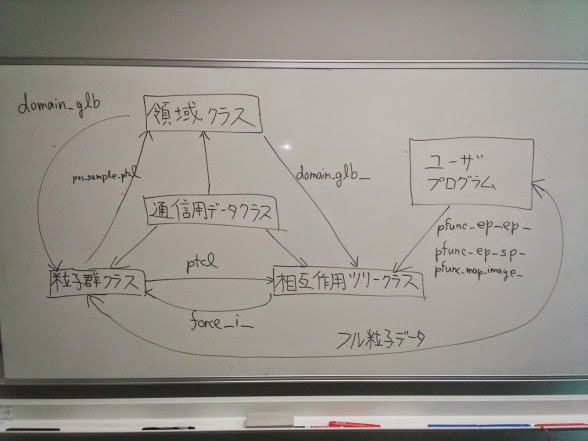
\includegraphics[width=10cm,bb=0 0 600 500]{fig/brief_interface.jpg}
    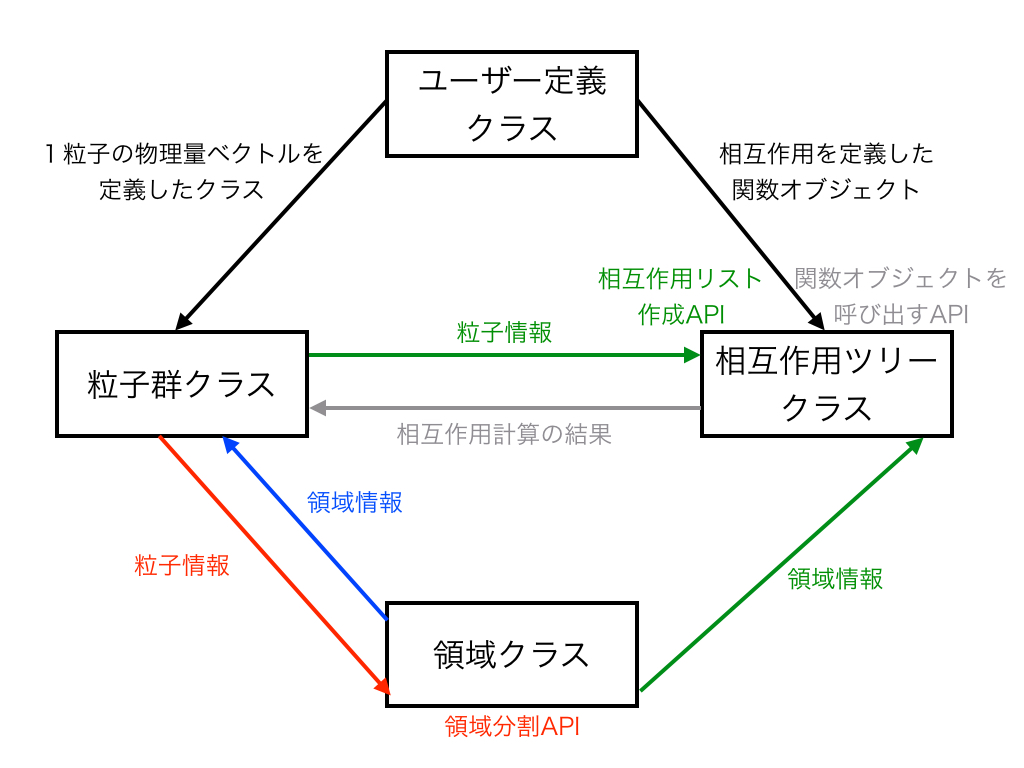
\includegraphics[width=10cm,bb=0 0 700 700]{fig/illustration/illustration.001.jpg}
  \end{center}
  \caption{モジュールインターフェースと情報の流れの模式図。}
  \label{fig:brief_interface}
\end{figure}

\newpage

%%%%%%%%%%%%%%%%%%%%%%%%%%%%%%%%%%%%%%%%%%%%%%%%%%%%%
\chapter{Fortran/C言語 インターフェースのファイル構成と概要}
\label{chap:file_str_and_ftn_if_overview}
この章では、FDPS Fortran/C言語 インターフェースのファイル構成と概要について記述する。はじめに
ソースファイルの構成とインターフェース概要について記述し、その後、ドキュメントとサンプルコードについて記述する。

%%%%%%%%%%%%%%%%%%%%%%%%%%%%%%%%%%%%%%%%%%%%%%%%%%%%
\section{ファイル構成と概要}
%%%%%%%%%%%%%%%%%%%%%%%%%
\subsection{FDPS 本体}
FDPS 本体のソースファイルはディレクトリ \path{src} の下にある。FDPS 本体は C++ で記述されており、FDPS の標準機能関係のソースファイルはすべて \path{src} の 直下にある。FDPS には拡張機能が用意されており、現時点では、Particle Mesh と x86 版 Phantom-GRAPE が実装されている。それぞれのソースファイルが、\path{src/particle_mesh} と \path{src/phantom_GRAPE_x86} にある。これら拡張機能は静的ライブラリとして使用される。そのため、各ディレクトリにおいて、ユーザ自身の手で、静的ライブラリを作成する必要がある。詳細はFDPS本体の仕様書(\path{doc/doc_specs_cpp_ja.pdf})をご覧頂きたい。
%%%%%%%%%%%%%%%%%%%%%%%%%
\subsection{Fortran インターフェース}
\label{subsec:file_str_ftn_if}
前節で述べた機能の内、Fortran から利用可能なのは、FDPS 標準機能(一部 API は除く)と拡張機能 Particle Mesh である。ユーザは Fortran インターフェースプログラムを通して、これらの機能を使用することとなる。この Fortran インターフェースは、ユーザがディレクトリ\path{scripts}の下に置かれたスクリプト\path{gen_ftn_if.py}を実行することで生成される(スクリプトの仕様は第\ref{chap:script_spec}章で解説する)。このインターフェース生成用スクリプトは、FDPSを利用するにあたってユーザ自身が定義(実装)しなければならない派生データ型(\textbf{ユーザ定義型};第\ref{chap:user_defined}章参照)を解析して、インターフェースプログラムを生成する。\uline{\textbf{したがって、ユーザ最初にしなければならないことはユーザ定義型の実装である}}。FDPSのFortran用のインターフェースがライブラリの形ではなく、このようなインターフェースプログラムの生成という形で提供される理由については別途第\ref{subsec:reasons_for_autogen_ftn_if}節で解説する。Fortranでユーザ定義型を実装するのに必要となるFortranファイルが\path{src/fortran_interface/modules}に、インターフェース生成時に設計図として使用されるファイル群が \path{src/fortran_interface/blueprints} に配置されている。

図\ref{fig:FDPS_ftn_if_file_str}に、Fortran用インターフェースプログラムの生成が正常に行われた場合の Fortran インターフェースのファイル構成とその役割を示している。図の破線で囲まれた4つのファイル(\path{FDPS_module.F90}, \path{FDPS_ftn_if.cpp}, \path{FDPS_Manipulators.cpp}, \path{main.cpp})がスクリプトによって生成されるFortranインターフェースプログラムであり、\path{f_main.F90}がユーザ側が用意するプログラムである。図の点線で囲まれたファイル(\path{FDPS_vector.F90}、\path{FDPS_matrix.F90}、\path{FDPS_super_particle.F90}等)は、前述したように、ユーザがユーザ定義型およびユーザ定義関数(第\ref{chap:overview}章参照)を記述するのに必要な派生データ型の定義を与える。以下、それぞれのインターフェースプログラムの役割について説明を行う。

%%% 図:全体のファイル構成
\begin{figure}[h]
\centering
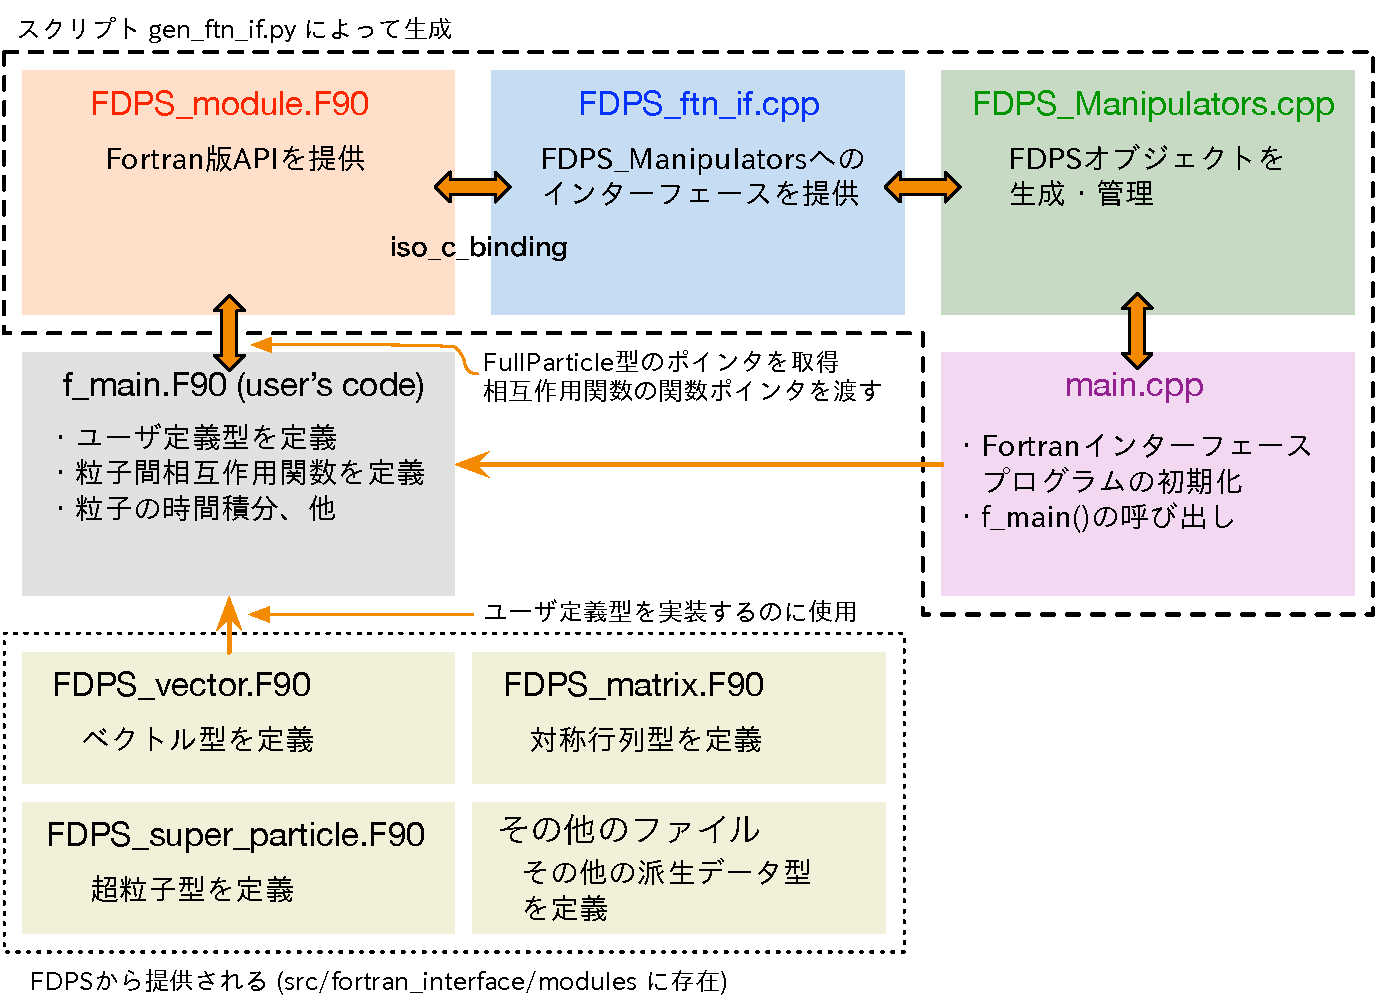
\includegraphics[width=\linewidth]{./fig/FDPS_ftn_if_file_str.pdf}
\caption{Fortran インターフェースとユーザコードの関係。}
\label{fig:FDPS_ftn_if_file_str}
\end{figure}


まず\path{FDPS_Manipulators.cpp}と\path{main.cpp}について説明する。FDPS 本体はC++で記述されているため、第\ref{chap:overview}章「FDPS 概要」で説明した領域クラス、粒子群クラス、相互作用ツリークラスのC++オブジェクトは、すべてC++ファイル内で生成し、管理する必要がある。これを行うのが、\path{FDPS_Manipulators.cpp}である。同様の理由によって、実行プログラムの\path{main}関数はC++ファイルに置く必要がある。そのため、\path{main.cpp}が生成される。この\path{main.cpp}では\path{f_main()}という名称のFortranのサブルーチンを呼び出す。したがって、ユーザはFortran サブルーチン \path{f_main()}を用意し、その中にユーザコードを実装する必要がある。詳細は第\ref{chap:API_spec_list}章「API 仕様一覧」に譲るが、\path{FDPS_Manipulators.cpp}で生成されるC++オブジェクトは、Fortranの整数変数に割り当てられる。したがって、ユーザはこれらのオブジェクトを整数変数を使って管理することとなる。

次に\path{FDPS_ftn_if.cpp}について説明する。FortranはC++の関数を直接呼び出して使用することはできないが、Fortran 2003の機能(Fortranモジュール\path{iso_c_binding}で提供される機能のこと)を使用することで、C言語の関数を呼び出すことが可能になる。そこで、本 FDPS Fortran インターフェースでは、\path{FDPS_Manipulators.cpp}内で定義される各種のC++関数のC言語インターフェースを別途用意し、これらをFortranから呼び出して、FDPSを操作する仕組みとした。これらC言語インターフェースが\path{FDPS_ftn_if.cpp}に実装されている。

最後に、\path{FDPS_module.F90}について説明する。\path{FDPS_module.F90}は、C言語インターフェースを呼び出すための派生データ型\path{FDPS_controller}をユーザに提供する。この\path{FDPS_controller}は、Fortran 2003のクラス(メンバ関数を持つ派生データ型のこと)であり、そのメンバ関数がFDPSのFortran用インターフェースを与える。メンバ関数、すなわち、Fortran インターフェースの一覧は第\ref{chap:API_spec_list}章「API 仕様一覧」で記述する。\path{FDPS_controller}は、\path{FDPS_module.F90}において、以下のように定義されている(リスト\ref{listing:FDPS_module_str}):
\begin{lstlisting}[caption=\texttt{FDPS\_module.F90}の構造,label=listing:FDPS_module_str]
module FDPS_module
   use, intrinsic :: iso_c_binding
   implicit none
   
   !**** FDPS controller
   type, public :: FDPS_controller
   contains
      !
      ! APIs are defined here.
      !
   end type FDPS_controller
   
end module FDPS_module  
\end{lstlisting}
見やすさのため、上記のリストにおいて、メンバ関数の宣言部の記述は省略している。実際には、各メンバ関数の宣言が、文字列\verb|contains|と文字列\verb|end type FDPS_controller|の間の領域に記述される。このような仕様のため、ユーザはユーザコードにおいて、以下の手順でFortranインターフェースを使用する必要がある:
\begin{enumerate}[leftmargin=*,itemsep=-1ex,label=(\arabic*)]
\item モジュール\path{FDPS_module}を\path{use}する
\item クラス\path{FDPS_controller}のオブジェクトを生成する
\item 生成した\path{FDPS_controller}オブジェクトのメンバ関数を呼び出す
\end{enumerate}
最も単純な使用例をリスト\ref{listing:simple_example_ftn_if}に示す:
\begin{lstlisting}[caption=Fortranインターフェースの使用例,label=listing:simple_example_ftn_if]
subroutine f_main()
   use FDPS_module ! Step (1)
   implicit none
   type(FDPS_controller) :: fdps_ctrl ! Step (2)
   
   ! Call Fortran interface
   call fdps_ctrl%PS_initialize() ! Step (3)
   
end subroutine f_main
\end{lstlisting}
リスト中にコメントで示された番号は、上の手順の番号に対応している。

%%%%%%%%%%%%%%%%%%%%%%%%%
\subsection{C言語 インターフェース}
\label{subsec:file_str_c_if}
C言語の場合もFortranの場合と全く同様に、C言語 インターフェースプログラムを通して、FDPSの機能を使用することになる。C言語 インターフェースプログラムの生成は、ユーザがディレクトリ\path{scripts}の下に置かれたスクリプト\path{gen_c_if.py}を実行することで行われる。このスクリプトは、FDPSを利用するにあたってユーザ自身が定義(実装)しなければならない構造体(同様に\textbf{ユーザ定義型}と呼称)を解析して、インターフェースプログラムを生成する。C言語でユーザ定義型を実装するのに必要となるC言語ヘッダーファイルが\path{src/c_interface/headers}に、インターフェース生成時に設計図として使用されるファイル群が \path{src/c_interface/blueprints} に配置されている。

図\ref{fig:FDPS_c_if_file_str}に、C言語用インターフェースプログラムの生成が正常に行われた場合の C言語 インターフェースのファイル構成とその役割を示している。図の破線で囲まれた4つのファイル(\path{FDPS_c_if.h}, \path{FDPS_ftn_if.cpp}, \path{FDPS_Manipulators.cpp}, \path{main.cpp})がスクリプトによって生成されるC言語インターフェースプログラムであり、\path{c_main.c}がユーザ側が用意するプログラムである。図の点線で囲まれたファイル(\path{FDPS_basic.h}、\path{FDPS_enum.h}、\path{FDPS_vector.h}、\path{FDPS_matrix.h}、\path{FDPS_super_particle.h}等)は、前述したように、ユーザがユーザ定義型およびユーザ定義関数(第\ref{chap:overview}章参照)を記述するのに必要な構造体の定義を与えるものである。図からわかるように、ファイル構成は、Fortranインターフェースプログラムと非常に類似した構成となっており(図\ref{fig:FDPS_ftn_if_file_str}参照)、特に同名のファイルの役割はFortranインターフェースで説明したファイルと全く同じである。以下、異なる部分についての注意書きのみを記す。


%%% 図:全体のファイル構成
\begin{figure}[h]
\centering
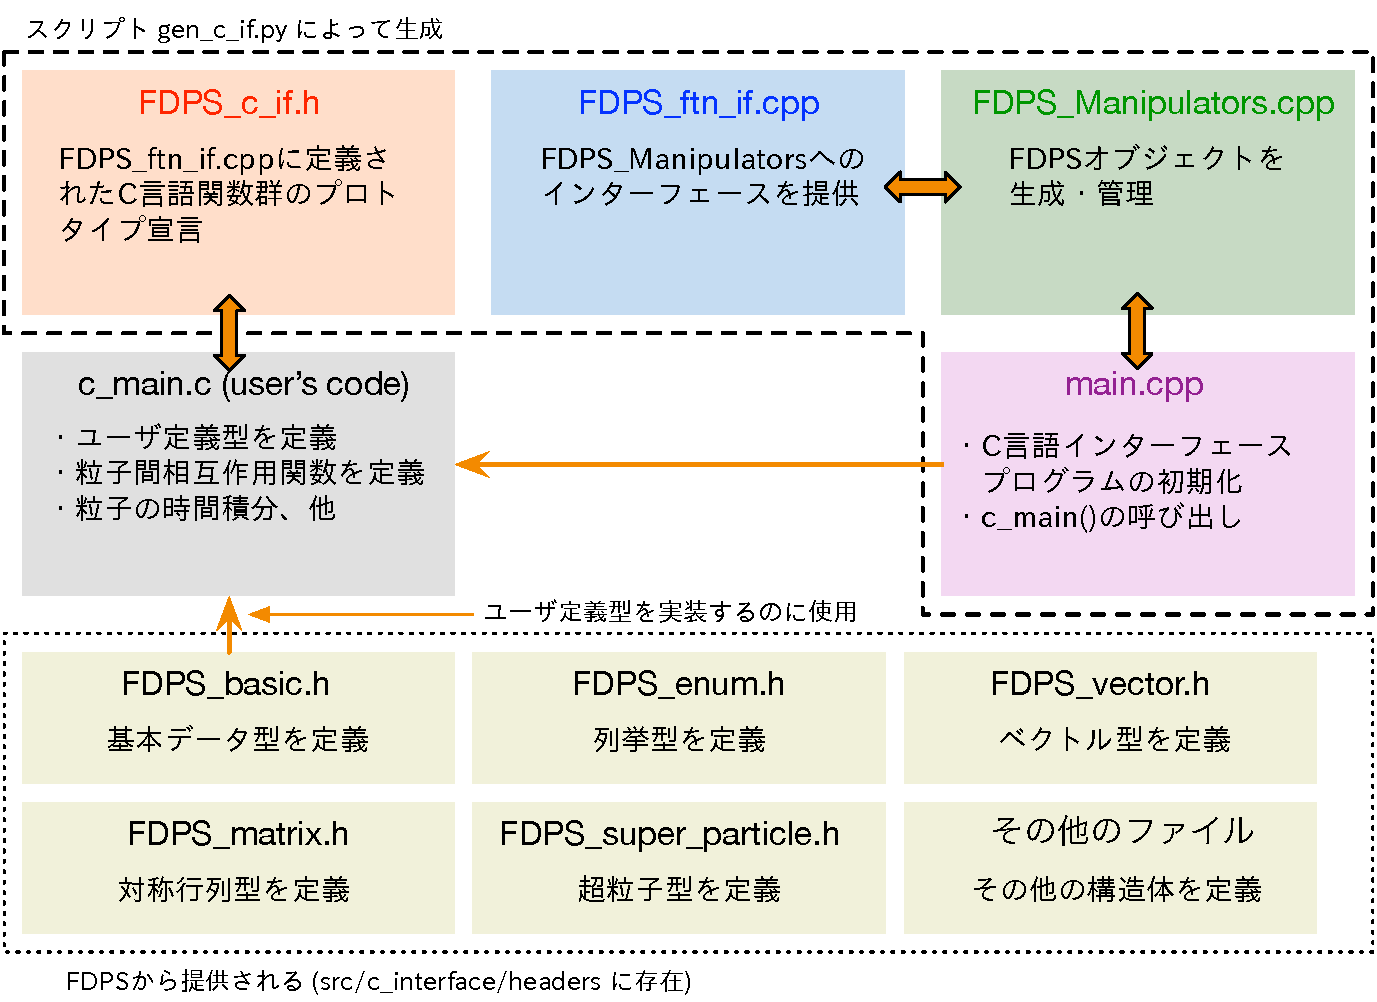
\includegraphics[width=\linewidth]{./fig/FDPS_c_if_file_str.pdf}
\caption{C言語 インターフェースとユーザコードの関係。}
\label{fig:FDPS_c_if_file_str}
\end{figure}

\begin{itemize}[leftmargin=*]
\item 実行ファイルの\path{main}関数は\path{main.cpp}にある。この\path{main.cpp}では\path{c_main()}という名称の\texttt{void}関数を呼び出す。したがって、ユーザは\texttt{void}関数 \path{c_main()}を用意し、その中にユーザコードを実装する必要がある。
\item FDPSのC言語用APIのプロトタイプ宣言は\path{FDPS_c_if.h}に記述されている。したがって、ユーザはFDPSの機能を利用するため、このファイルをインクルードする必要がある。\path{FDPS_c_if.h}では、FDPSが提供する構造体の定義が記述されたヘッダーファイル群(\path{FDPS_basic.h}等)がインクルードされているため、ユーザはこのファイルのみをインクルードすれば、これら構造体をユーザコードの中で利用することができる。
\end{itemize}


%%%%%%%%%%%%%%%%%%%%%%%%%
\subsection{Fortran/C言語 インターフェースを使ったコード開発の流れ}
本節では、FDPSのFortran/C言語 インターフェースを使ったユーザコード開発の流れについて記述する。大まかな流れは以下のようになる:
\begin{enumerate}[leftmargin=*,label={[\arabic*]}]
\litem{ユーザ定義型の実装} 前節で述べた通り、FDPSのFortran/C言語 インターフェースを生成するためには、はじめにユーザ定義型を実装しなければならない。ユーザ定義型はFortranでFDPSを利用する場合には派生データ型で、C言語でFDPSを利用する場合には構造体として実装する。ユーザ定義型の記述方法の詳細は、第\ref{chap:user_defined}章で説明する。
\litem{インターフェースプログラムの生成} ユーザ定義型の実装が完了したら、インターフェース生成用スクリプト \path{gen_ftn_if.py} または \path{gen_c_if.py} を使って、インターフェースプログラムを生成する。生成が完了した時点で、ユーザはFDPSのFortran/C言語用インターフェースをユーザコードの中で使用することができるようになる。スクリプトの使用法と仕様については第\ref{chap:script_spec}章で説明する。
\litem{ユーザ定義関数の実装} ユーザは相互作用を記述する関数(ユーザ定義関数)を実装しなければならない。ユーザ定義関数は、Fortranではサブルーチン、C言語では\texttt{void}関数として実装する。ユーザ定義関数の記述方法の詳細は、第\ref{chap:user_defined}章で説明する。
\litem{ユーザコードの開発} ユーザ定義型、ユーザ定義関数、FDPS APIを用いて、ユーザが行いたい粒子シミュレーションコードを開発する。この際、次の点に注意して開発を行う必要がある:
\begin{itemize}
\item ユーザコードはFortranのサブルーチン\path{f_main()}、或いは、C言語の\texttt{void}関数 \path{c_main()}の中に実装しなければならない。
\item FDPS Fortran インターフェースのAPIは、クラス\path{FDPS_controller}のメンバ関数として提供される。したがって、FDPS APIはメンバ関数を呼び出して使用する。一方、FDPS C言語 インターフェースのAPIのプロトタイプ宣言は、\path{FDPS_c_if.h}でなされているため、このファイルをインクルードすることでAPIを呼び出すことが可能となる。
\end{itemize}
Fortran インターフェースを用いたコードの例に関しては、\path{sample/fortran}の下で提供されているサンプルコードを参照して頂きたい(第\ref{sec:sample_codes}節も参照のこと)。一方、C言語 インターフェースを用いたサンプルコードは、\path{sample/c}の下に用意されている。
\litem{コンパイル} ユーザコードの実装が完了したら、コンパイルを行い、実行プログラムを得る。前節で述べたように、インターフェースプログラムはC++言語と、Fortran言語或いはC言語のソースファイルが混在した構成となっており、単一の言語のみで構成されたプログラムとは異なる仕方でコンパイルする必要がある。この点に関しての詳細は、第\ref{chap:compile_and_macro}章で解説する。FDPSではコンパイル時のマクロ定義を使い、いくつかの設定を行うことが可能である。これに関しても、第\ref{chap:compile_and_macro}章で解説する。拡張機能 Particle Mesh を使用する場合には、事前に必要なライブラリをインストールし、コンパイル時に適切にライブラリを指定することが必要である。
\litem{実行} コンパイルして得られる実行ファイルは、通常の実行ファイルと違いはない。ユーザが利用している計算機環境の利用規則に則って、実行ファイルを実行する。
\end{enumerate}

%%%%%%%%%%%%%%%%%%%%%%%%%
\subsection{インターフェースプログラム生成の必要性}
\label{subsec:reasons_for_autogen_ftn_if}
前々節で述べたように、FDPSのFortran/C言語用インターフェースはライブラリの形で提供されるものではなく、インターフェースプログラムのソースコードの形で提供される。本節では、この理由について解説を行う。

まず、準備として、C++でのFDPSの使用について概説する。第\ref{chap:overview}章\ref{subsec:things_to_do_by_users}節で述べた通り、FDPSではユーザは粒子や相互作用の定義を自由に行うことができ、これによって、FDPSは様々なタイプの粒子シミュレーションに対して適用可能となっている。この自由度を実現するため、FDPS 本体の関数はC++のテンプレート機能を用いて記述されている。ここで、テンプレート機能とは、Fortranでいうサブルーチンや関数(或いはC言語の関数)に、(変数ではなく)データ型を引数として受け取れるようにする機能のことである。この機能によって、C++では仮のデータ型を使用して関数を記述することが可能となる(この仮のデータ型はコンパイル時に具体的なデータ型になってさえいればよい)。また、FDPS 本体はC++のヘッダファイルの形で提供される。したがって、C++でFDPSを使用する場合、ユーザはFDPSのヘッダファイルをユーザコードの中でインクルードし、FDPS APIのテンプレート引数にユーザが定義した粒子型を指定して使用する。ユーザコードのコンパイル時には、FDPS APIの関数で使用されるすべての変数のデータ型が決定されているため、コンパイラは問題なくユーザプログラムをコンパイルすることが可能となっているのである。

FortranやC言語にはテンプレート機能に相当するものは存在しないため、仮の(或いは、未定の)データ型を用いてサブルーチンや関数を実装する、ということはFortranやC言語では不可能である。これが、Fortran/C言語用インターフェースをライブラリの形で提供できない1つの理由である。我々は、FortranやC言語においてもユーザが粒子や相互作用の定義を自由に行えるようにするため、ユーザが実装した粒子の派生データ型/構造体等を調べ、それに応じて適切なAPIを自動的に生成する方法を採用している。

もう1つの理由は、C++で実装されたFDPSをそのまま使用しているからである。C++で記述されたFDPSとFortran 或いは C言語のプログラムの間でデータをやり取りするためには、FortranやC言語で記述された粒子型と同等な粒子クラスをC++側に用意する必要がある。これにもユーザが実装した派生データ型や構造体を解析して生成するという作業が必要となる。

以上の理由により、FDPS Fortran/C言語 インターフェースは、ソースコードで提供される形となっている。

%%%%%%%%%%%%%%%%%%%%%%%%%%%%%%%%%%%%%%%%%%%%%%%%%%%%
\section{ドキュメント}
ドキュメント関係のファイルはディレクトリ \path{doc} の下にある。サンプルコードを使ってFDPS Fortran インターフェースの基本的な使用法を解説するチュートリアル文書が \path{doc_tutorial_ftn_ja.pdf} である。C言語 インターフェースの基本的な使用方法についてのチュートリアル文書は\path{doc_tutorial_c_ja.pdf}である。仕様書(本文書)が \path{doc_specs_ftn_ja.pdf} である。

%%%%%%%%%%%%%%%%%%%%%%%%%%%%%%%%%%%%%%%%%%%%%%%%%%%%
\section{サンプルコード}
\label{sec:sample_codes}
FortranとC言語のサンプルコードが、それぞれ、ディレクトリ \path{sample/fortran} 及び \path{sample/c} の下にある。サンプルコードは4つ用意されており、それぞれ、無衝突系の重力 $N$ 体シミュレーションコード(\path{sample/fortran/nbody}, \path{sample/c/nbody})、固定長カーネルを使った SPH シミュレーションコード(\path{sample/fortran/sph}, \path{sample/c/sph})、$\mathrm{P^{3}M}$(Particle-Particle-Particle-Mesh) 計算用コード(\path{sample/fortran/p3m}, \path{sample/c/p3m})、円盤銀河の$N$体/SPHシミュレーションコード(\path{sample/fortran/nbody+sph}, \path{sample/c/nbody+sph})となっている。

\newpage

%%%%%%%%%%%%%%%%%%%%%%%%%%%%%%%%%%%%%%%%%%%%%%%%%%%%%
\chapter{FDPSで提供されるデータ型}
\label{chap:data_types}
FDPS Fortran/C interface defines several data types including vector types, symmetric matrix types, superparticle types, time profile type, enum types. In addition, basic data types are also defined in C. These data types are required to be used in user-defined types and user-defined functions (Chap.~\ref{chap:user_defined}) or are used as returned values in some APIs (Chap.~\ref{chap:API_spec_list}).

%%%%%%%%%%%%%%%%%%%%%%%%%%%%%%%%%%%%%%%%%%%%%%%%%%%%%%
\section{Basic data types {\small (C only)}}
\label{sec:basic_types}
FDPS C interface defines six basic data types: \path{fdps_s32}, \path{fdps_u32}, \path{fdps_f32}, \path{fdps_s64}, \path{fdps_u64}, \path{fdps_f64}. They are defined in the file \path{src/c_interface/headers/FDPS_basic.h} as follows (Listing~\ref{listing:basic_types}). These data types are used to defined other data types provided by FDPS.

\begin{lstlisting}[language=C,caption=Basic data types (C only),label=listing:basic_types]
#pragma once

/* 32 bit data types */
typedef int          fdps_s32;
typedef unsigned int fdps_u32;
#ifdef PARTICLE_SIMULATOR_ALL_64BIT_PRECISION
typedef double       fdps_f32;
#else
typedef float        fdps_f32;
#endif

/* 64 bit data types */
typedef long long int          fdps_s64;
typedef unsigned long long int fdps_u64;
typedef double                 fdps_f64;
\end{lstlisting}

\redtext{Note that the macro \texttt{PARTICLE\_SIMULATOR\_ALL\_64BIT\_PRECISION} is just introduced for future and C interface programs work correctly only if this macro is undefined.}

%%%%%%%%%%%%%%%%%%%%%%%%%%%%%%%%%%%%%%%%%%%%%%%%%%%%%%
\section{Vector types}
\label{sec:vector_types}
FDPS Fortran and C interface define two types of vector: \path{fdps_f32vec} and \path{fdps_f64vec}. They are defined in the files \path{src/fortran_interface/modules/FDPS_vector.F90} and \path{src/c_interface/headers/FDPS_vector.h} as follows (Listings~\ref{listing:vector_types} and \ref{listing:vector_types_in_C}). Each vector has 2 or 3 member variables depending on the spatial dimension of the simulation. By default, the spatial dimension of the simulation is assumed to be 3, but it is 2 if the macro \path{PARTICLE_SIMULATOR_TWO_DIMENSION} is defined at the compilation. The data type of the member variables is either 32-bit or 64-bit floating point numbers.

\begin{lstlisting}[caption=Vector types (Fortran),label=listing:vector_types]
module fdps_vector
   use, intrinsic :: iso_c_binding
   implicit none
   
   type, public, bind(c) :: fdps_f32vec
#ifdef PARTICLE_SIMULATOR_TWO_DIMENSION 
      real(kind=c_float) :: x,y
#else
      real(kind=c_float) :: x,y,z
#endif
   end type fdps_f32vec

   type, public, bind(c) :: fdps_f64vec
#ifdef PARTICLE_SIMULATOR_TWO_DIMENSION 
      real(kind=c_double) :: x,y
#else
      real(kind=c_double) :: x,y,z
#endif
   end type fdps_f64vec

end module fdps_vector
\end{lstlisting}

\begin{lstlisting}[language=C,caption=Vector types (C), label=listing:vector_types_in_C]
#pragma once
#include "FDPS_basic.h"

//**** PS::F32vec
typedef struct  {
#ifdef PARTICLE_SIMULATOR_TWO_DIMENSION
   fdps_f32 x,y;
#else
   fdps_f32 x,y,z;
#endif
} fdps_f32vec;

//**** PS::F64vec
typedef struct  {
#ifdef PARTICLE_SIMULATOR_TWO_DIMENSION
   fdps_f64 x,y;
#else
   fdps_f64 x,y,z;
#endif
} fdps_f64vec;
\end{lstlisting}

In Fortran, for the vector types, the definitions of the assignment (\texttt{=}) and the arithmetic operators (\texttt{+},\texttt{-},\texttt{*},\texttt{/}) are extended as shown in Table.~\ref{tbl:op_ext:fdps_vector}. For more details, see \path{FDPS_vector.F90}.

\begin{table}[H]
\begin{tabularx}{\linewidth}{|c|c|c|X|}
\toprule
\rowcolor{Snow2}
Symbol & Left-hand side & Right-hand side & Definition \\
\midrule
% 代入記号(=)
\multirow{3}{*}{\texttt{=}} & vector & scalar$^{\dagger}$ & \multirow{3}{\hsize}{\footnotesize Assign RHS to LHS$^{\sharp}$. When RHS is scalar, it is assigned to all the components of LHS. When RHS is an array, each component of LHS is assigned by array element according to the memory ordering.} \\[2pt]
\cmidrule(r){2-3}
 & vector & array of scalars$^{\ddagger}$ &  \\[2pt]
\cmidrule(r){2-3}
 & vector & vector &  \\[2pt]
\midrule
% + 演算子
\multirow{4}{*}{\texttt{+}} & vector & array of scalars & \multirow{3}{\hsize}{\footnotesize Addition of LHS and RHS. When one of the operands is an array, it is assumed that each element of the array corresponds to the component of the vector according to the memory ordering.} \\[2pt]
\cmidrule(r){2-3}
 & array of scalars & vector & \\[2pt]
\cmidrule(r){2-3}
 & vector & vector & \\[2pt]
\cmidrule(r){2-4}
 & none & vector & Do nothing \\
\midrule
% - 演算子
\multirow{4}{*}{\texttt{-}} & vector & array of scalars & \multirow{3}{\hsize}{\footnotesize Subtraction RHS from LHS. When one of the operands is an array, it is assumed that each element of the array corresponds to the component of the vector according to the memory ordering.} \\[2pt]
\cmidrule(r){2-3}
& array of scalars & vector &  \\[2pt]
\cmidrule(r){2-3}
& vector & vector & \\[2pt]
\cmidrule(r){2-4}
& none & vector & Inversion of the sign of the vector \\
\midrule
% * 演算子
\multirow{5}{*}{\texttt{*}} & vector & scalar & \multirow{2}{*}{Scalar-vector product} \\
\cmidrule(r){2-3}
 & scalar & vector & \\
\cmidrule(r){2-4}
 & vector & array of scalars & \multirow{3}{\hsize}{\footnotesize Inner product. When one of the operands is an array, it is assumed that each element of the array corresponds to the component of the vector according to the memory ordering.} \\
\cmidrule(r){2-3}
 & array of scalars & vector &  \\
\cmidrule(r){2-3}
 & vector & vector &  \\
\midrule
\texttt{/} & vector & scalar & Division LHS by RHS. \\
\bottomrule
\end{tabularx}
\begin{flushleft}
$^{\dagger}$ The data type of scalar must be one of intrinsic data types in Fortran and be numeric. \\
$^{\ddagger}$ The size of array must be 2 if the macro \path{PARTICLE_SIMULATOR_TWO_DIMENSION} is defined at the compilation. Otherwise, it must be 3. \\
$^{\sharp}$ LHS and RHS stand for the left- and the right-hand sides, respectively.
\end{flushleft}
\caption{The definitions of the assignment and the arithmetic operators extended for the vector types}
\label{tbl:op_ext:fdps_vector}
\end{table}


%%%%%%%%%%%%%%%%%%%%%%%%%%%%%%%%%%%%%%%%%%%%%%%%%%%%%%
\section{Symmetric Matrix types}
\label{sec:symmetric_matrix_types}
There are two types of symmetric matrix: \path{fdps_f32mat} and \path{fdps_f64mat}. These are defined in the files \path{src/fortran_interface/modules/FDPS_matrix.F90} and \path{src/c_interface/headers/FDPS_matrix.h} as follows (Listings~\ref{listing:symmetric_matrix_types} and \ref{listing:symmetric_matrix_types_in_C}). Each symmetric matrix type has 3 or 6 member variables depending on the spatial dimension of the simulation. By default, the spatial dimension of the simulation is assumed to be 3, but it is 2 if the macro \path{PARTICLE_SIMULATOR_TWO_DIMENSION} is defined at the compilation. The data type of the member variables is either 32-bit or 64-bit floating point numbers.

\begin{lstlisting}[caption=Symmetric Matrix types (Fortran),label=listing:symmetric_matrix_types]
module fdps_matrix
   use, intrinsic :: iso_c_binding
   implicit none

   !**** PS::F32mat
   type, public, bind(c) :: fdps_f32mat
#ifndef PARTICLE_SIMULATOR_TWO_DIMENSION
      real(kind=c_float) :: xx,yy,zz,xy,xz,yz
#else
      real(kind=c_float) :: xx,yy,xy
#endif
   end type fdps_f32mat

   !**** PS::F64mat
   type, public, bind(c) :: fdps_f64mat
#ifndef PARTICLE_SIMULATOR_TWO_DIMENSION
      real(kind=c_double) :: xx,yy,zz,xy,xz,yz
#else
      real(kind=c_double) :: xx,yy,xy
#endif
   end type fdps_f64mat

end module fdps_matrix  
\end{lstlisting}

\begin{lstlisting}[language=C,caption=Symmetric Matrix types (C), label=listing:symmetric_matrix_types_in_C]
#pragma once
#include "FDPS_basic.h"

//**** PS::F32mat
typedef struct {
#ifndef PARTICLE_SIMULATOR_TWO_DIMENSION
   fdps_f32 xx,yy,zz,xy,xz,yz;
#else
   fdps_f32 xx,yy,xy;
#endif
} fdps_f32mat;

//**** PS::F64mat
typedef struct {
#ifndef PARTICLE_SIMULATOR_TWO_DIMENSION
   fdps_f64 xx,yy,zz,xy,xz,yz;
#else
   fdps_f64 xx,yy,xy;
#endif
} fdps_f64mat;
\end{lstlisting}

In Fortran, for the symmetric matrix types, the definitions of the assignment (\texttt{=}) and the arithmetic operators (\texttt{+},\texttt{-},\texttt{*},\texttt{-}) are extended as shown in Table.~\ref{tbl:op_ext:fdps_matrix}. For more details, see \path{FDPS_matrix.F90}.

\begin{table}[H]
\begin{tabularx}{\linewidth}{|c|c|c|X|}
\toprule
\rowcolor{Snow2}
Symbol & Left-hand side & Right-hand side & Definition \\
\midrule
% = 記号
\multirow{2}{*}{\texttt{=}}& matrix & scalar$^{\dagger}$ & \multirow{2}{\hsize}{\footnotesize Assign RHS to LHS. When RHS is scalar, it is assigned to all the components of LHS.} \\
\cmidrule(r){2-3}
& matrix & matrix & \\
\midrule
% + 演算子
\multirow{2}{*}{\texttt{+}} & matrix & matrix & Addition of LHS and RHS. \\
\cmidrule(r){2-4}
& none & matrix & Do nothing \\
\midrule
% - 演算子
\multirow{2}{*}{\texttt{-}} & matrix & matrix & Subtraction RHS from LHS. \\
\cmidrule(r){2-4}
& none & matrix & {\footnotesize Sign inversion of all the components of the matrix} \\
\midrule
% * 演算子
\multirow{3}{*}{\texttt{*}} & matrix & scalar & \multirow{2}{*}{Scalar-matrix product} \\
\cmidrule(r){2-3}
 & scalar & matrix &  \\
\cmidrule(r){2-4}
 & matrix & matrix & Matrix product \\
\midrule
% / 演算子
\texttt{/} & matrix & scalar & Division LHS by RHS. \\
\bottomrule
\end{tabularx}
\begin{flushleft}
$^{\dagger}$ The data type of scalar must be one of intrinsic data types in Fortran and be numeric.
\end{flushleft}
\caption{The definitions of the assignment and the arithmetic operators extended for the symmetric matrix types}
\label{tbl:op_ext:fdps_matrix}
\end{table}



%%%%%%%%%%%%%%%%%%%%%%%%%%%%%%%%%%%%%%%%%%%%%%%%%%%%%%
\section{Superparticle types}
\label{sec:super_particle_types}
A superparticle is a virtual particle that represents a group of real particles, which are located far from the $i$-particle (a particle which we want to calculate the force acting on). Its properties are computed from the properties of these real particles via some way. Superparticle types are derived data types required to describe the interaction between a particle and a superparticle. They are used in user-defined functions to receive data of superparticles.

The superparticle types include \path{fdps_spj_monopole},\path{fdps_spj_quadrupole},\path{fdps_spj_monopole_geomcen},\path{fdps_spj_dipole_geomcen},\path{fdps_spj_quadrupole_geomcen},\path{fdps_spj_monopole_scatter},\path{fdps_spj_quadrupole_scatter}, \path{fdps_spj_monopole_symmetry}, \path{fdps_spj_quadrupole_symmetry},  \path{fdps_spj_monopole_cutoff}. They are defined in the files \path{src/fortran_interface/modules/FDPS_super_particle.F90} and \path{src/c_interface/headers/FDPS_super_particle.h} as follows (Listings~\ref{listing:superparticle_types} and \ref{listing:superparticle_types_in_C}). Note that the vector types and the symmetric matrix types are used to define the superparticle types.

\begin{lstlisting}[caption=Superparticle types (Fortran),label=listing:superparticle_types]
module fdps_super_particle
   use, intrinsic :: iso_c_binding
   use fdps_vector
   use fdps_matrix
   implicit none

   !**** PS::SPJMonopole
   type, public, bind(c) :: fdps_spj_monopole
      real(kind=c_double) :: mass
      type(fdps_f64vec) :: pos
   end type fdps_spj_monopole

   !**** PS::SPJQuadrupole
   type, public, bind(c) :: fdps_spj_quadrupole
      real(kind=c_double) :: mass
      type(fdps_f64vec)  :: pos
      type(fdps_f64mat)  :: quad
   end type fdps_spj_quadrupole

   !**** PS::SPJMonopoleGeometricCenter
   type, public, bind(c) :: fdps_spj_monopole_geomcen
      integer(kind=c_long_long) :: n_ptcl
      real(kind=c_double) :: charge
      type(fdps_f64vec) :: pos
   end type fdps_spj_monopole_geomcen

   !**** PS::SPJDipoleGeometricCenter
   type, public, bind(c) :: fdps_spj_dipole_geomcen
      integer(kind=c_long_long) :: n_ptcl
      real(kind=c_double) :: charge
      type(fdps_f64vec) :: pos
      type(fdps_f64vec) :: dipole
   end type fdps_spj_dipole_geomcen

   !**** PS::SPJQuadrupoleGeometricCenter
   type, public, bind(c) :: fdps_spj_quadrupole_geomcen
      integer(kind=c_long_long) :: n_ptcl
      real(kind=c_double) :: charge
      type(fdps_f64vec) :: pos
      type(fdps_f64vec) :: dipole
      type(fdps_f64mat) :: quadrupole
   end type fdps_spj_quadrupole_geomcen

   !**** PS::SPJMonopoleScatter
   type, public, bind(c) :: fdps_spj_monopole_scatter
      real(kind=c_double) :: mass
      type(fdps_f64vec) :: pos
   end type fdps_spj_monopole_scatter

   !**** PS::SPJQuadrupoleScatter
   type, public, bind(c) :: fdps_spj_quadrupole_scatter
      real(kind=c_double) :: mass
      type(fdps_f64vec)  :: pos
      type(fdps_f64mat)  :: quad
   end type fdps_spj_quadrupole_scatter

   !**** PS::SPJMonopoleSymmetry
   type, public, bind(c) :: fdps_spj_monopole_symmetry
      real(kind=c_double) :: mass
      type(fdps_f64vec) :: pos
   end type fdps_spj_monopole_symmetry

   !**** PS::SPJQuadrupoleSymmetry
   type, public, bind(c) :: fdps_spj_quadrupole_symmetry
      real(kind=c_double) :: mass
      type(fdps_f64vec) :: pos
      type(fdps_f64mat) :: quad
   end type fdps_spj_quadrupole_symmetry

   !**** PS::SPJMonopoleCutoff
   type, public, bind(c) :: fdps_spj_monopole_cutoff
      real(kind=c_double) :: mass
      type(fdps_f64vec) :: pos
   end type fdps_spj_monopole_cutoff
   
end module fdps_super_particle   
\end{lstlisting}

\begin{lstlisting}[language=C,caption=Superparticle types (C),label=listing:superparticle_types_in_C]
#pragma once
#include "FDPS_basic.h"
#include "FDPS_vector.h"
#include "FDPS_matrix.h"

#ifdef PARTICLE_SIMULATOR_SPMOM_F32
typedef fdps_s32    fdps_sSP;
typedef fdps_f32    fdps_fSP;
typedef fdps_f32vec fdps_fSPvec;
typedef fdps_f32mat fdps_fSPmat;
#else
typedef fdps_s64    fdps_sSP;
typedef fdps_f64    fdps_fSP;
typedef fdps_f64vec fdps_fSPvec;
typedef fdps_f64mat fdps_fSPmat;
#endif

//**** PS::SPJMonopole
typedef struct {
   fdps_fSP mass;
   fdps_fSPvec pos;
} fdps_spj_monopole;

//**** PS::SPJQuadrupole
typedef struct {
   fdps_fSP mass;
   fdps_fSPvec pos;
   fdps_fSPmat quad;
} fdps_spj_quadrupole;

//**** PS::SPJMonopoleGeometricCenter
typedef struct {
   fdps_sSP n_ptcl;
   fdps_fSP charge;
   fdps_fSPvec pos;
} fdps_spj_monopole_geomcen;

//**** PS::SPJDipoleGeometricCenter
typedef struct {
   fdps_sSP n_ptcl;
   fdps_fSP charge;
   fdps_fSPvec pos;
   fdps_fSPvec dipole;
} fdps_spj_dipole_geomcen;

//**** PS::SPJQuadrupoleGeometricCenter
typedef struct {
   fdps_sSP n_ptcl;
   fdps_fSP charge;
   fdps_fSPvec pos;
   fdps_fSPvec dipole;
   fdps_fSPmat quadrupole;
} fdps_spj_quadrupole_geomcen;

//**** PS::SPJMonopoleScatter
typedef struct {
   fdps_fSP mass;
   fdps_fSPvec pos;
} fdps_spj_monopole_scatter;

//**** PS::SPJQuadrupoleScatter
typedef struct {
   fdps_fSP mass;
   fdps_fSPvec pos;
   fdps_fSPmat quad;
} fdps_spj_quadrupole_scatter;

//**** PS::SPJMonopoleSymmetry
typedef struct {
   fdps_fSP mass;
   fdps_fSPvec pos;
} fdps_spj_monopole_symmetry;

//**** PS::SPJQuadrupoleSymmetry
typedef struct {
   fdps_fSP mass;
   fdps_fSPvec pos;
   fdps_fSPmat quad;
} fdps_spj_quadrupole_symmetry;

//**** PS::SPJMonopoleCutoff
typedef struct {
   fdps_fSP mass;
   fdps_fSPvec pos;
} fdps_spj_monopole_cutoff;
\end{lstlisting}

There is an one-to-one correspondence between the superparticle types and the types of tree objects. Accordingly, users must use an appropriate superparticle type corresponding to the type of created tree object. The correspondence relationship between the types of tree objects and the superparticle types is shown in Table~\ref{tbl:tree_and_super_particle}. Note that the types of tree object for short-range force are not shown in this table, because superparticle is only used in the case of long-range force. For the other types of tree object and the way to create tree objects, see Chap.~\ref{chap:API_spec_list} \S~\ref{sec:tree_APIs}.

\begin{landscape}
\begin{table}[h]
\begin{tabularx}{\hsize}{lp{5cm}Xl}
\toprule
\rowcolor{Snow2}
Tree type & Highest-order of multipole moments$^{\dagger}$ & Range of interaction & Superparticle type \\
\midrule
Long-Monopole type & monopole(CoM) & Entire region & \path{fdps_spj_monopole} \\
\midrule
Long-Quadrupole type & quadrupole(CoM) & Entire region & \path{fdps_spj_quadrupole} \\
\midrule
Long-MonopoleGeometricCenter type & monopole(GC) & Entire region & \path{fdps_spj_monopole_geomcen} \\
\midrule
Long-DipoleGeometricCenter type & dipole(GC) & Entire region & \path{fdps_spj_dipole_geomcen} \\
\midrule
Long-QuadrupoleGeometricCenter type & quadrupole(GC) & Entire region & \path{fdps_spj_quadrupole_geomcen} \\
\midrule
Long-MonopoleWithScatterSearch type$^{\ddagger}$ & monopole(CoM) & Entire region & \path{fdps_spj_monopole_scatter} \\
\midrule
Long-QuadrupoleWithScatterSearch type$^{\ddagger}$ & quadrupole(CoM) & Entire region & \path{fdps_spj_quadrupole_scatter} \\
\midrule
Long-MonopoleWithSymmetrySearch type$^{\ddagger}$ & monopole(CoM) & Entire region & \path{fdps_spj_monopole_symmetry} \\
\midrule
Long-QuadrupoleWithSymmetrySearch type$^{\ddagger}$ & quadrupole(CoM) & Entire region & \path{fdps_spj_quadrupole_symmetry} \\
\midrule
Long-MonopoleWithCutoff type & monopole(CoM) & Within cutoff radius & \path{fdps_spj_monopole_cutoff} \\
\bottomrule
\end{tabularx}
\begin{flushleft}
$^{\dagger}$ CoM indicates that multipole moments are calculated assuming that the center-of-mass is the center of the expansion. GC indicates that multipole moments are calculated assuming that the geometric center is the center of the expansion. \\
$^{\ddagger}$ Scatter- or Symmetry-mode neighbor search is possible. In the calculation of interaction, neighbor particles are forcibly treated as normal particles. In other words, superparticles do not have neighbor particles as members.
\end{flushleft}
\caption{The correspondence relationship between the types of tree for long-range force and the superparticle types}
\label{tbl:tree_and_super_particle}
\end{table}
\end{landscape}


%%%%%%%%%%%%%%%%%%%%%%%%%%%%%%%%%%%%%%%%%%%%%%%%%%%%%%
\section{Time profile types}
\label{sec:time_profile_types}
Time profile types are used to obtain the elapsed times of various types of calculations performed in FDPS. At present, there is only one time profile type \path{fdps_time_profile}. It is defined in the files \path{src/fortran_interface/modules/FDPS_time_profile.F90} and \path{src/c_interface/headers/FDPS_time_profile.h} as follows (Listings~\ref{listing:time_profile_types} and \ref{listing:time_profile_types_in_C}). This data type is exclusively used by the APIs for time measurement (for detail, see Chap.~\ref{chap:API_spec_list}).

\begin{lstlisting}[caption=Time profile types (Fortran),label=listing:time_profile_types]
module fdps_time_profile
   use, intrinsic :: iso_c_binding
   implicit none

   !**** PS::TimeProfile
   type, public, bind(c) :: fdps_time_prof
      real(kind=c_double) :: collect_sample_particle
      real(kind=c_double) :: decompose_domain
      real(kind=c_double) :: exchange_particle
      real(kind=c_double) :: set_particle_local_tree
      real(kind=c_double) :: set_particle_global_tree
      real(kind=c_double) :: make_local_tree
      real(kind=c_double) :: make_global_tree
      real(kind=c_double) :: set_root_cell
      real(kind=c_double) :: calc_force
      real(kind=c_double) :: calc_moment_local_tree
      real(kind=c_double) :: calc_moment_global_tree
      real(kind=c_double) :: make_LET_1st
      real(kind=c_double) :: make_LET_2nd
      real(kind=c_double) :: exchange_LET_1st
      real(kind=c_double) :: exchange_LET_2nd
                                                                                                   
      real(kind=c_double) :: morton_sort_local_tree                                                
      real(kind=c_double) :: link_cell_local_tree                                                  
      real(kind=c_double) :: morton_sort_global_tree                                               
      real(kind=c_double) :: link_cell_global_tree                                                 
                                                                                                   
      real(kind=c_double) :: make_local_tree_tot                                                   
      ! = make_local_tree + calc_moment_local_tree                                                 
      real(kind=c_double) :: make_global_tree_tot                                                  
      real(kind=c_double) :: exchange_LET_tot                                                      
      ! = make_LET_1st + make_LET_2nd + exchange_LET_1st + exchange_LET_2nd                        
                                                                                                   
      real(kind=c_double) :: calc_force__core__walk_tree                                           
                                                                                                   
      real(kind=c_double) :: calc_force__make_ipgroup                                              
      real(kind=c_double) :: calc_force__core                                                      
      real(kind=c_double) :: calc_force__copy_original_order                                       
                                                                                                   
      real(kind=c_double) :: exchange_particle__find_particle                                       
      real(kind=c_double) :: exchange_particle__exchange_particle

      real(kind=c_double) :: decompose_domain__sort_particle_1st
      real(kind=c_double) :: decompose_domain__sort_particle_2nd
      real(kind=c_double) :: decompose_domain__sort_particle_3rd
      real(kind=c_double) :: decompose_domain__gather_particle

      real(kind=c_double) :: decompose_domain__setup
      real(kind=c_double) :: decompose_domain__determine_coord_1st
      real(kind=c_double) :: decompose_domain__migrae_particle_1st
      real(kind=c_double) :: decompose_domain__determine_coord_2nd
      real(kind=c_double) :: decompose_domain__determine_coord_3rd
      real(kind=c_double) :: decompose_domain__exchange_pos_domain

      real(kind=c_double) :: exchange_LET_1st__a2a_n
      real(kind=c_double) :: exchange_LET_1st__icomm_sp
      real(kind=c_double) :: exchange_LET_1st__a2a_sp
      real(kind=c_double) :: exchange_LET_1st__icomm_ep
      real(kind=c_double) :: exchange_LET_1st__a2a_ep
   end type fdps_time_prof

end module fdps_time_profile  
\end{lstlisting}

\begin{lstlisting}[language=C,caption=Time profile types (C),label=listing:time_profile_types_in_C]
//**** PS::TimeProfile
typedef struct {
   double collect_sample_particle;
   double decompose_domain;
   double exchange_particle;
   double set_particle_local_tree;
   double set_particle_global_tree;
   double make_local_tree;
   double make_global_tree;
   double set_root_cell;
   double calc_force;
   double calc_moment_local_tree;
   double calc_moment_global_tree;
   double make_LET_1st;
   double make_LET_2nd;
   double exchange_LET_1st;
   double exchange_LET_2nd;
   double write_back;

   double morton_sort_local_tree;
   double link_cell_local_tree;
   double morton_sort_global_tree;
   double link_cell_global_tree;

   double make_local_tree_tot; // = make_local_tree + calc_moment_local_tree
   double make_global_tree_tot;
   double exchange_LET_tot; // = make_LET_1st + make_LET_2nd + exchange_LET_1st + exchange_LET_2nd

   double calc_force__core__walk_tree;
   double calc_force__core__keep_list;
   double calc_force__core__copy_ep;
   double calc_force__core__dispatch;
   double calc_force__core__retrieve;

   double calc_force__make_ipgroup;
   double calc_force__core;
   double calc_force__copy_original_order;

   double exchange_particle__find_particle;
   double exchange_particle__exchange_particle;
   
   double decompose_domain__sort_particle_1st;
   double decompose_domain__sort_particle_2nd;
   double decompose_domain__sort_particle_3rd;
   double decompose_domain__gather_particle;

   double decompose_domain__setup;
   double decompose_domain__determine_coord_1st;
   double decompose_domain__migrae_particle_1st;
   double decompose_domain__determine_coord_2nd;
   double decompose_domain__determine_coord_3rd;
   double decompose_domain__exchange_pos_domain;

   double exchange_LET_1st__a2a_n;
   double exchange_LET_1st__icomm_sp;
   double exchange_LET_1st__a2a_sp;
   double exchange_LET_1st__icomm_ep;
   double exchange_LET_1st__a2a_ep;

   double add_moment_as_sp_local;
   double add_moment_as_sp_global;
} fdps_time_prof;
\end{lstlisting}

%%%%%%%%%%%%%%%%%%%%%%%%%%%%%%%%%%%%%%%%%%%%%%%%%%%%%%
\section{Enumerated types}
\label{sec:enum_types}
In this section, we describe enumerated types defined in FDPS Fortran/C interface.

%%%%%%%%%%%%%%%%%%%%%%%%%%%
\subsection{Boundary condition types}
\label{subsec:enum_bc}
Boundary condition types are used in the APIs \path{set_boundary_condition} {\small (Fortran)} and \path{fdps_set_boundary_condition} {\small (C)} to specify the boundary condition of simulation (see \S~\ref{sec:dinfo_APIs} ``APIs for DomainInfo object" in Chap.~\ref{chap:API_spec_list}). It is defined in the files \path{FDPS_module.F90} and \path{src/c_interface/headers/FDPS_enum.h} as follows.

\begin{lstlisting}[caption=Boundary condition types (Fortran)]
module FDPS_module
   use, intrinsic :: iso_c_binding
   implicit none
   
   !* Enum types
   !**** PS::BOUNDARY_CONDITION
   enum, bind(c)
      enumerator :: fdps_bc_open
      enumerator :: fdps_bc_periodic_x
      enumerator :: fdps_bc_periodic_y
      enumerator :: fdps_bc_periodic_z
      enumerator :: fdps_bc_periodic_xy
      enumerator :: fdps_bc_periodic_xz
      enumerator :: fdps_bc_periodic_yz
      enumerator :: fdps_bc_periodic_xyz
      enumerator :: fdps_bc_shearing_box
      enumerator :: fdps_bc_user_defined
   end enum
   
end module FDPS_module
\end{lstlisting}

\begin{lstlisting}[language=C,caption=Boundary condition types (C)]
typedef enum {
   FDPS_BC_OPEN,
   FDPS_BC_PERIODIC_X,
   FDPS_BC_PERIODIC_Y,
   FDPS_BC_PERIODIC_Z,
   FDPS_BC_PERIODIC_XY,
   FDPS_BC_PERIODIC_XZ,
   FDPS_BC_PERIODIC_YZ,
   FDPS_BC_PERIODIC_XYZ,
   FDPS_BC_SHEARING_BOX,
   FDPS_BC_USER_DEFINED,
} FDPS_BOUNDARY_CONDITION;
\end{lstlisting}


Table~\ref{tbl:boundary_conditions} shows the relations between the enumerators of the boundary condition types in Fortran and boundary conditions. Users can obtain the same kind of the table for the boundary condition types in C if capitalizing the names of the enumerators in the table.

\begin{table}[H]
\begin{tabularx}{\linewidth}{cX}
\toprule
\rowcolor{Snow2}
Enumerator & Boundary condition \\
\midrule
\path{fdps_bc_open} &  The open boundary condition. \textbf{This is the default boundary condition in FDPS}. \\
\midrule
\path{fdps_bc_periodic_x} & The periodic boundary condition in the direction of $x$-axis, and the open boundary condition in other directions. FDPS assume that the lower and upper boundaries of the computational box (or the interval) along $x$-axis are closed and open, respectively (i.e. \texttt{[)}). This is assumed for all periodic boundary conditions. \\
\midrule
\path{fdps_bc_periodic_y} & The periodic boundary condition in the direction of $y$-axis, and the open boundary condition in other directions. \\
\midrule
\path{fdps_bc_periodic_z} & The periodic boundary condition in the direction of $z$-axis, and the open boundary condition in other directions. \\
\midrule
\path{fdps_bc_periodic_xy} & The periodic boundary condition in the directions of $x$- and $y$-axes, and the open boundary condition in the direction of $z$-axis. \\
\midrule
\path{fdps_bc_periodic_xz} & The periodic boundary condition in the directions of $x$- and $z$-axes, and the open boundary condition in the direction of $y$-axis. \\
\midrule
\path{fdps_bc_periodic_yz} & The periodic boundary condition in the directions of $y$- and $z$-axes, and the open boundary condition in the direction of $x$-axis. \\
\midrule
\path{fdps_bc_periodic_xyz} & The periodic boundary condition in all three directions. \\
\midrule
\path{fdps_bc_shearing_box} & The shearing-box boundary condition (\textcolor{red}{Not implemented yet}). \\
\midrule
\path{fdps_bc_user_defined} & User-defined boundary condition (\textcolor{red}{Not implemented yet}). \\
\bottomrule
\end{tabularx}
\caption{The correspondence relation between the enumerator of the boundary condition types and the boundary conditions}
\label{tbl:boundary_conditions}
\end{table}

%%%%%%%%%%%%%%%%%%%%%%%%%%%
\subsection{Interaction list mode types}
\label{subsec:enum_list_mode}
Interaction list mode types are used to determine whether we reuse interaction lists at interaction calculations. These types are used as an argument in the APIs \path{calc_force_all_and_write_back} and \path{calc_force_all} in Fortran or \path{fdps_calc_force_all_and_write_back} and \path{fdps_calc_force_all} in C (see \S~\ref{sec:tree_APIs} `APIs for Tree object`" in Chap.~\ref{chap:API_spec_list}) and are defined in the files \path{FDPS_module.F90} and \path{src/c_interface/headers/FDPS_enum.h} as follows.

\begin{lstlisting}[caption=Interaction list mode types (Fortran)]
module FDPS_module
   use, intrinsic :: iso_c_binding
   implicit none
   
   !* Enum types
   !**** PS::INTERACTION_LIST_MODE
   enum, bind(c)
      enumerator :: fdps_make_list
      enumerator :: fdps_make_list_for_reuse
      enumerator :: fdps_reuse_list
   end enum
   
end module FDPS_module
\end{lstlisting}

\begin{lstlisting}[language=C,caption=Interaction list mode types (C)]
typedef enum {
   FDPS_MAKE_LIST,
   FDPS_MAKE_LIST_FOR_REUSE,
   FDPS_REUSE_LIST,
} FDPS_INTERACTION_LIST_MODE;  
\end{lstlisting}

Table \ref{tbl:interaction_list_mode} shows the relations between the enumerators of the interaction list mode types in Fortran and operation mode of the APIs described above. Users can obtain the same kind of the table for the interaction list mode types in C if capitalizing the name of the enumerators in the table.

\begin{table}[h]
\begin{tabularx}{\linewidth}{cX}
\toprule
\rowcolor{Snow2}
Enumerator & Operation mode \\
\midrule
\path{fdps_make_list} & FDPS (re)makes interaction lists for each interaction calculation (each call of the APIs described above). In this case, we cannot reuse interaction list in the next interaction calculation because FDPS does not store the information of interaction list. \textbf{This is the default operation mode in FDPS}.\\
\midrule
\path{fdps_make_list_for_reuse} & FDPS (re)makes interaction lists and stores them internally. Then, it performs interaction calculation. In this case, we can reuse these interaction lists in the next interaction calculation if we call the APIs with the flag \path{fdps_reuse_list}. The interaction lists memorized in FDPS are destroyed if we perform the interaction calculation with the flags \path{fdps_make_list_for_reuse} or \path{fdps_make_list}.\\
\midrule
\path{fdps_reuse_list} & FDPS performs interaction calculation using the previously-created interaction lists, which are the lists that are created at the previous call of the APIs with the flag \path{fdps_make_list_for_reuse}. In this case, moment information in superparticles are automatically updated using the latest particle information.\\
\bottomrule
\end{tabularx}
\caption{The correspondence relation between the enumerator of the interaction list mode types and the operation modes}
\label{tbl:interaction_list_mode}
\end{table}



%%%%%%%%%%%%%%%%%%%%%%%%%%%
\subsection{CALC\_DISTANCE\_TYPE type}
\label{subsec:enum_calc_distance_type}
The {\tt CALC\_DISTANCE\_TYPE} type is used to specify the way the
distances between particles are calculated during treewalk. 
This type is defined in \path{FDPS_module.F90} (Fortran)
and \path{src/c_interface/headers/FDPS_enum.h} (C) as follows.

\begin{lstlisting}[caption={\tt CALC\_DISTANCE\_TYPE} type (Fortran)]
module FDPS_module
   use, intrinsic :: iso_c_binding
   implicit none
   
   !**** PS::CALC_DISTANCE_TYPE
   enum, bind(c)
     enumerator :: fdps_calc_distance_type_normal
     enumerator :: fdps_calc_distance_type_nearest_x
     enumerator :: fdps_calc_distance_type_nearest_y
     enumerator :: fdps_calc_distance_type_nearest_xy
     enumerator :: fdps_calc_distance_type_nearest_z
     enumerator :: fdps_calc_distance_type_nearest_xz
     enumerator :: fdps_calc_distance_type_nearest_yz
     enumerator :: fdps_calc_distance_type_nearest_xyz
   end enum
   
end module FDPS_module
\end{lstlisting}

\begin{lstlisting}[language=C,caption={\tt CALC\_DISTANCE\_TYPE} type (C)]
typedef enum {
    FDPS_CALC_DISTANCE_TYPE_NORMAL = 0,
    FDPS_CALC_DISTANCE_TYPE_NEAREST_X = 1,
    FDPS_CALC_DISTANCE_TYPE_NEAREST_Y = 2,
    FDPS_CALC_DISTANCE_TYPE_NEAREST_XY = 3,
    FDPS_CALC_DISTANCE_TYPE_NEAREST_Z = 4,
    FDPS_CALC_DISTANCE_TYPE_NEAREST_XZ = 5,
    FDPS_CALC_DISTANCE_TYPE_NEAREST_YZ = 6,
    FDPS_CALC_DISTANCE_TYPE_NEAREST_XYZ = 7,
} FDPS_CALC_DISTANCE_TYPE;
\end{lstlisting}

The default is the NORMAL type, for which the usual Cartesian distance
(L2 norm) is used for distance calculation in tree walk.
When types with X, Y or Z are used, for specified coordinates,
the minimum image with the assumption of periodic boundary is used for
tree walk.

%%%%%%%%%%%%%%%%%%%%%%%%%%%
\subsection{EXCHANGE\_LET\_MODE type}
\label{subsec:enum_exchange_let_mode}
The {\tt EXCHANGE\_LET\_MODE} type is used to specify the
communication algorithm used for the exchange of LET.

This type is defined in \path{FDPS_module.F90} (Fortran)
and \path{src/c_interface/headers/FDPS_enum.h} (C) as follows.

\begin{lstlisting}[caption={\tt EXCHANGE\_LET\_MODE} type (Fortran)]
module FDPS_module
   use, intrinsic :: iso_c_binding
   implicit none
   
   !**** PS::EXCHANGE_LET_MODE
   enum, bind(c)
     enumerator :: fdps_exchange_let_a2a
     enumerator :: fdps_exchange_let_p2p_exact
     enumerator :: fdps_exchange_let_p2p_fast
   end enum
   
end module FDPS_module
\end{lstlisting}

\begin{lstlisting}[language=C,caption={\tt EXCHANGE\_LET\_MODE} type (C)]
typedef enum {
    EXCHANGE_LET_A2A,
    EXCHANGE_LET_P2P_EXACT,
    EXCHANGE_LET_P2P_FAST,
}EXCHANGE_LET_MODE;
\end{lstlisting}

When {\tt EXCHANGE\_LET\_A2A} is specified, 
{\tt MPI\_Alltoall} is used for LET exchange.


When {\tt EXCHANGE\_LET\_P2P\_EXACT} is specified,
instead of {\tt MPI\_Alltoall}, a combination of {\tt MPI\_Allgather}
and {\tt MPI\_Isend/recv}is used. On systems with relatively slow {\tt
MPI\_Alltoall}, or with very large number of processes, this mode
might be faster. This mode gives the result the same as that for
EXCHANGE\_LET\_A2A up to round-off error.


When {\tt EXCHANGE\_LET\_P2P\_FAST} is specified,
instead of {\tt MPI\_Alltoall}, a combination of {\tt MPI\_Allgather}
and {\tt MPI\_Isend/recv}is used. This mode gives the result not
exactly the same as that for
EXCHANGE\_LET\_A2A, but faster than
{\tt EXCHANGE\_LET\_P2P\_EXACT}.

\newpage

%%%%%%%%%%%%%%%%%%%%%%%%%%%%%%%%%%%%%%%%%%%%%%%%%%%%%
\chapter{ユーザー定義型・ユーザー定義関数}
\label{chap:user_defined}
本章では、ユーザーが定義しなければならない派生データ型(Fortran) 或いは 構造体(C言語) (\textbf{ユーザ定義型})と相互作用関数(\textbf{ユーザ定義関数})について記述する。ユーザー定義型には、FullParticle 型、EssentialParticleI 型、EssentialParticleJ 型、Force 型がある。また、ユーザー定義関数には、粒子-粒子相互作用を記述する calcForceEpEpと、粒子-超粒子間相互作用を記述する calcForceEpSp がある。本章で記述するのは、ユーザ定義型やユーザ定義関数を定義する際の規定である。FDPS は、ユーザ定義型が粒子の位置等、粒子計算に必須の物理量を持つことを仮定する。したがって、ユーザは FDPS に必須物理量がユーザ定義型のどのメンバ変数に対応するかを教える必要がある。また、FDPS 内部では、ユーザ定義型の間でデータのやりとりを行うが、それをユーザが指定した方法で行うことになる。したがって、ユーザはその方法をコードに書く必要がある。これらFDPSへの指示や方法の記述はすべてコード内に特別な指示文(\textbf{FDPS 指示文})を記述することによって行う。以下、まずはじめにユーザ定義型について記述し、その後ユーザ定義関数について記述する。

%%%%%%%%%%%%%%%%%%%%%%%%%%%%%%%%%%%%%%%%%%%%%%%%%%%%%
\section{ユーザ定義型}
\label{sec:user_defined_types}
まず概要を述べる。FullParticle 型は、ある1粒子の情報すべてを持つ派生データ型(Fortran) 或いは 構造体(C言語) であり、粒子群クラスのオブジェクトの生成に使用されるものである (第\ref{chap:overview}章\ref{sec:overview_action}節の手順0)。EssentialParticleI 型、EssentialParticleJ 型、Force 型は粒子間の相互作用の定義を補助するものであり、それぞれ、相互作用を計算する際に$i$粒子に必要な情報、相互作用を計算する際に$j$粒子に必要な情報、相互作用の結果の情報を持つ派生データ型(Fortran) 或いは 構造体(C言語)である。これらは FullParticle 型のサブセットであるため、これらを FullParticle 型で代用することも可能である。しかし、FullParticle 型は相互作用の定義に必要のないデータを多く含む場合も考えられるため、計算コストを軽減したいならば、これらの型を使用することを検討するべきである。

以下では、はじめにユーザ定義型を記述する上での共通の規則について記述する。その後、FullParticle型、EssentialParticleI型、EssentialParticleJ型、Force型の順で記述する。

%%%%%%%%%%%%%%%%%%%%%%%%%%%
\subsection{共通規則}
\label{subsec:common_rules_for_user_defined_types}
%%%%
\subsubsection{Fortran 文法に関する要請}
\label{s2sec:requirements_for_fortran_grammer}
本節では、ユーザ定義型となるために派生データ型が満たすべき最低限のFortran文法について記述する。第\ref{chap:file_str_and_ftn_if_overview}章で述べた通り、本 FDPS Fortran インターフェースは、FDPSのC言語インターフェースを通して、FDPS 本体とデータをやり取りする。このため、すべてのユーザ定義型はC言語と(Fortran 2003 標準で)\textbf{interoperable}である必要がある。具体的には、ユーザ定義型となる派生データ型は次の条件を満たしている必要がある:
\begin{enumerate}[leftmargin=*,itemsep=-1ex,label=(\arabic*)]
\item 派生データ型は\path{bind(c)}属性を持たなければならない。
\item すべてのメンバ変数がinteroperableなデータ型である。Fortran 2003 標準(ISO/IEC 1539-1:2004(E))で定義される「C言語とinteroperableな」データ型の一覧は本書表\ref{tbl:interoperable_data_types}や言語仕様書の第15節「Interoperability with C」で確認できる\footnote{Fortranの言語仕様書を販売している\href{http://www.iso.org/iso/home.htm}{ISO} (International Organization for Standardization)からはFortran 2008 Standard (ISO/IEC 1539-1:2010(E))のみ購入可能である。}ほか、\href{https://gcc.gnu.org/wiki/HomePage}{GCC Wiki}のページ\href{https://gcc.gnu.org/wiki/GFortranStandards}{GFortranStandards}で紹介されている各種非公式文書(ドラフト段階の言語仕様書)やGNU gfortranの\href{https://gcc.gnu.org/onlinedocs/gfortran/ISO_005fC\_005fBINDING.html#ISO\_005fC\_005fBINDING}{オンラインドキュメント}でも解説されている。「C言語とinteroperable」な派生データ型をメンバ変数として持つことは可能である。
\item すべてのメンバ変数は\path{allocatable}属性を持たない。
\item すべてのメンバ変数は\path{pointer}属性を持たない。
\item メンバ関数を持たない。
\end{enumerate}
加えて、FDPS 側からの要請として、次の条件を満たす必要がある:
\begin{enumerate}[leftmargin=*,itemsep=-1ex,label=(\arabic*),resume]
\item 派生データ型はモジュール内で定義されている。
\item 派生データ型は\path{public}属性を持つ。
\item メンバ変数として持たせることが可能な派生データ型はベクトル型と対称行列型(第\ref{chap:data_types}章参照)のみである。
\item 派生データ型は多次元配列をメンバ変数として持てない(これは将来のバージョンにおいて対応する予定である)。
\item メンバ変数の(1次元)配列の形状を指定する場合、\texttt{dimension}文で指定するか、変数名に\texttt{(配列要素数)}を付けるかの、\underbold{どちらか片方の}方法でなければならない。
\end{enumerate}
以上の条件が、派生データ型がユーザ定義型となるために満たす必要があるFortran 文法である。これに加え、次節\ref{subsubsec:FDPS_directives}で説明するFDPS指示文によって、どのユーザ定義型(FullParticle型,EssentialParticleI型,EssentialParticleJ型,Force型)に対応するかや、必須物理量がどのメンバ変数に対応しているか等を指定してはじめてユーザ定義型となる。

%%%%
\subsubsection{C言語 文法に関する要請}
\label{s2sec:requirements_for_c_grammer}
本節では、ユーザ定義型となるために構造体が満たすべき最低限のC言語文法について記述する。第\ref{chap:file_str_and_ftn_if_overview}章で述べた通り、C言語インターフェースプログラムの1つ\path{FDPS_ftn_if.cpp}は、Fortranインターフェースでも共用される。このため、自由に構造体を定義できるわけではなく、前節\ref{s2sec:requirements_for_fortran_grammer}で述べたような制限を受ける。具体的には、ユーザ定義型となる構造体は次の条件を満たさなければならない:
\begin{enumerate}[leftmargin=*,itemsep=-1ex,label=(\arabic*)]
\item 構造体はタグ名を持つ必要がある。タグ名はすべて小文字でなければならない。
\item メンバ変数のデータ型として利用できるのは、(i) Fortran 2003 標準(ISO/IEC 1539-1:2004(E))と相互運用可能なデータ型(詳細は第\ref{s2sec:requirements_for_fortran_grammer}節の(2)、及び本書表\ref{tbl:interoperable_data_types}を参照のこと)、(ii) ベクトル型、(iii) 対称行列型のみである。\textbf{特に、符号なし整数、及び、あらゆるポインタは持てないことに注意して頂きたい}。
\item 構造体は多次元配列をメンバ変数として持てない(これは将来のバージョンにおいて対応する予定である)。
\item メンバ変数名はすべて小文字でなければならない。
\end{enumerate}

Fortranの場合と同様、これに加え、次節\ref{subsubsec:FDPS_directives}で説明するFDPS指示文を付け加えて、はじめてユーザ定義型の資格を得る。

\subsubsection{FDPS 指示文 (共通項目のみ)}
\label{subsubsec:FDPS_directives}
本節では、すべてのユーザ定義型に共通して使用可能なFDPS指示文の概要と記述方法について解説する。各ユーザ定義型に固有の指示文に関しては、第\ref{subsec:FullParticle}〜\ref{subsec:Force}節で解説する。

FDPS指示文には以下の3つの種類がある:
\begin{enumerate}[leftmargin=*,itemsep=-1ex,label=(\alph*)]
\item 派生データ型/構造体がどのユーザ定義型に対応するかを指定する指示文。\label{enum:FDPS_str_dir}
\item 派生データ型/構造体のメンバ変数がどの必須物理量に対応するかを指定する指示文。\label{enum:FDPS_mbr_dir}
\item ユーザ定義型同士のデータ移動の方法を指定する指示文。\label{enum:FDPS_meth_dir}
\end{enumerate}
これらの指示文の内、以下で、最初の2つ\ref{enum:FDPS_str_dir},\ref{enum:FDPS_mbr_dir}について解説する。以降の解説では、まず、FortranにおけるFDPS指示文の書き方について説明し、その後、C言語の場合を説明する。

\subsubsubsection{ユーザ定義型の種別を指定するFDPS 指示文}
派生データ型\textit{\texttt{type\_name}}がどのユーザ定義型に対応するかを指定するには、次の書式の指示文を記述する:
\begin{screen}
\begin{Verbatim}[commandchars=\\\{\}]
type, public, bind(c) :: \vrbit{type_name} !\$fdps \vrbit{keyword}
end type [\vrbit{type_name}]
\end{Verbatim}
\end{screen}

或いは、

\begin{screen}
\begin{Verbatim}[commandchars=\\\{\}]
!\$fdps \vrbit{keyword}
type, public, bind(c) :: \vrbit{type_name}
end type [\vrbit{type_name}]
\end{Verbatim}
\end{screen}
ここで[]は、その中身が省略可能であることを示す記号である。FDPS指示文は必ず文字列\verb|!$fdps|で開始される。英字はすべて小文字でなければならない。!で始まることからわかるように、FDPS指示文は単なるコメント文であり、Fortranプログラムの動作に影響を与えるものではない。インターフェース生成スクリプトだけが、このコメント文を指示文として解釈する。\verb|!$fdps|に半角スペースを置いて続く\textit{\texttt{keyword}}は、ユーザ定義型を指定するための文字列である。可能なキーワードは、\path{FP}, \path{EPI}, \path{EPJ}, \path{Force}であり、大文字・小文字を区別する。それぞれFullParticle型、EssentialParticleI型、EssentialParticleJ型、Force型に対応している。FDPS指示文は派生データ型名の右側か、1つ前の行に記述しなければならない。FDPS指示文の中で改行を行うことはできない。第\ref{sec:user_defined_types}節で述べた通り、EssentialParticleI型、EssentialParticleJ型、Force型はFullParticle型のサブセットでり、FullParticle型がこれら3つを兼ねることが可能である。その場合には、以下のリスト\ref{listing:FDPS_str_dir_example}に示されるように、キーワードをカンマで区切って並べればよい:
\begin{lstlisting}[caption=FullParticle型が他を兼ねる場合の例,label=listing:FDPS_str_dir_example]
type, public, bind(c) :: full_particle !$fdps FP,EPI,EPJ,Force
end type full_particle
\end{lstlisting}
FullParticle型がEssentialParticleI型だけを兼ねるといったことも可能である。

構造体 \textit{\texttt{tag\_name}}がどのユーザ定義型に対応するかを指定するには、次の書式の指示文を記述する:
\begin{screen}
\begin{Verbatim}[commandchars=\\\{\}]
struct \vrbit{tag_name} \{ //\$fdps \vrbit{keyword}
\};
\end{Verbatim}
\end{screen}

或いは、

\begin{screen}
\begin{Verbatim}[commandchars=\\\{\}]
//\$fdps \vrbit{keyword}
struct \vrbit{tag_name} \{
\};
\end{Verbatim}
\end{screen}
指示文の書き方はFortranの場合とほぼ同じである。違いのみ以下に示す。
\begin{itemize}[leftmargin=*]
\item コメント文からコメント記号と先頭の空白文字をすべて取り除いたときに得られる文字列が、文字列\verb|$fdps|で開始される場合(後続の文字列と空白文字で区切られている必要がある)、そのコメント文は指示文として解釈される。上の例では、コメント記号\texttt{//}を使っているが、別のコメント記号\texttt{/*},\texttt{*/}を使って、\texttt{/* \$fdps */}のように記述してもよい。
\item 指示文\ref{enum:FDPS_str_dir}と解釈されるのは、\texttt{struct}の直前の指示文、或いは、\textit{\texttt{tag\_name}}の後の最初の指示文である。指示文はどちらか一方の位置に記述しなければならない。
\end{itemize}


\subsubsubsection{必須物理量を指定するFDPS指示文}
次に、必須物理量に対応するメンバ変数を指定する指示文\ref{enum:FDPS_mbr_dir}について解説する。FDPSでは必須物理量として、粒子の電荷量(質量)、粒子の位置が必要である。また、ある種の粒子シミュレーションでは探索半径も必要となる。派生データ型\textit{\texttt{type\_name}}のメンバ変数\textit{\texttt{mbr\_name}}がどの必須物理量に対応するかを指定するには、次の書式の指示文を記述する:
\begin{screen}
\begin{Verbatim}[commandchars=\\\{\}]
type, public, bind(c) :: \vrbit{type_name}
   \vrbit{data_type} :: \vrbit{mbr_name} !\$fdps \vrbit{keyword}
end type [\vrbit{type_name}]
\end{Verbatim}
\end{screen}

或いは、

\begin{screen}
\begin{Verbatim}[commandchars=\\\{\}]
type, public, bind(c) :: \vrbit{type_name}
   !\$fdps \vrbit{keyword}
   \vrbit{data_type} :: \vrbit{mbr_name} 
end type [\vrbit{type_name}]
\end{Verbatim}
\end{screen}
ここでは、見やすさのため、ユーザ定義型の種別を指定する指示文は省略している。指示文は、指示文の開始を示す文字列\verb|!$fdps|で始まり、半角スペースを置いて\textit{\texttt{keyword}}が続く。可能なキーワードは、\path{id}、\path{charge}、\path{position}、\path{rsearch}、\path{velocity}である\footnote{但し、\path{velocity}は予約語であり、現時点で生成されるインターフェースプログラムの内容に影響しない}。それぞれ、粒子の識別番号、粒子の電荷量(質量)、粒子の位置、粒子の探索半径、粒子の速度に対応している。キーワードはすべて小文字でなければならない。また、1つのメンバ変数に対して1つの指示文を対応させなければならない。指示文は、変数名の右側か1つ前の行に記述しなければならない。

メンバ変数のデータ型\textit{\texttt{data\_type}}は、対応する必須物理量が持つべきデータ型に一致していなければならない。以下に、各必須物理量が持つべきデータ型をまとめる:
\begin{table}[H]
\begin{tabularx}{\linewidth}{cX}
\toprule
\rowcolor{Snow2}
物理量名 & 可能なデータ型 \\
\midrule
粒子の識別番号 & \texttt{integer(kind=c\_long\_long)} \\
\midrule
\multirow{2}{*}{電荷(質量)および探索半径} & \texttt{real(kind=c\_float)} \\
 & \texttt{real(kind=c\_double)} \\
\midrule
\multirow{4}{*}{位置および速度} & \texttt{type(fdps\_f32vec)} \\
& \texttt{real(kind=c\_float), dimension(space\_dim)}$^{\dagger}$ \\
& \texttt{type(fdps\_f64vec)} \\
& \texttt{real(kind=c\_double), dimension(space\_dim)}$^{\dagger}$ \\
\bottomrule
\end{tabularx}
\begin{flushleft}
$^{\dagger}$ \texttt{space\_dim}は空間次元を表す。コンパイル時にマクロ\path{PARTICLE_SIMULATOR_TWO_DIMENSION}が定義されている場合は2、それ以外は3である必要がある(第\ref{chap:compile_and_macro}章参照)。
\end{flushleft}
\caption{各必須物理量が持つべきデータ型。}
\end{table}


構造体\textit{\texttt{tag\_name}}のメンバ変数\textit{\texttt{mbr\_name}}がどの必須物理量に対応するかを指定するには、次の書式の指示文を記述する:
\begin{screen}
\begin{Verbatim}[commandchars=\\\{\}]
struct \vrbit{tag_name} \{
   \vrbit{data_type} \vrbit{mbr_name}; //\$fdps \vrbit{keyword}
\};
\end{Verbatim}
\end{screen}

或いは、

\begin{screen}
\begin{Verbatim}[commandchars=\\\{\}]
struct \vrbit{tag_name} \{
   //\$fdps \vrbit{keyword}
   \vrbit{data_type} \vrbit{mbr_name};
\};
\end{Verbatim}
\end{screen}

指示文の書き方はFortranの場合と同じである。各必須物理量が持つべきデータ型は、上の表に記載されたFortranのデータ型をC言語のデータ型に適切に読み替えることで得られる(表\ref{tbl:interoperable_data_types}を参照のこと)。



\subsubsubsection{FDPS指示文の記述例}
最後に、FullParticle型の実装例を示す(リスト\ref{listing:FP_example}および\ref{listing:FP_example_in_C})。この例ではここで説明しなかったFDPS指示文\ref{enum:FDPS_meth_dir}が使用されているが、FDPS指示文\ref{enum:FDPS_str_dir},\ref{enum:FDPS_mbr_dir}がどのように使用されているかに注意してほしい。

\begin{lstlisting}[caption=ユーザ定義型の例 (Fortran),label=listing:FP_example]
module user_defined_types
   use, intrinsic :: iso_c_binding
   use :: fdps_vector
   implicit none
   
   !**** Full particle type
   type, public, bind(c) :: full_particle !$fdps FP,EPI,EPJ,Force
      !$fdps copyFromForce full_particle (pot,pot) (acc,acc)
      !$fdps copyFromFP full_particle (id,id) (mass,mass) (eps,eps) (pos,pos) 
      integer(kind=c_long_long) :: id !$fdps id
      real(kind=c_double) :: mass !$fdps charge
      real(kind=c_double) :: eps
      type(fdps_f64vec) :: pos !$fdps position
      type(fdps_f64vec) :: vel !$fdps velocity
      real(kind=c_double) :: pot
      type(fdps_f64vec) :: acc
   end type full_particle

end module user_defined
\end{lstlisting}

\begin{lstlisting}[language=C,caption=ユーザ定義型の例 (C言語),label=listing:FP_example_in_C]
#include "FDPS_c_if.h"
   
//**** Full particle type
typedef struct full_particle { //$fdps FP,EPI,EPJ,Force
   //$fdps copyFromForce full_particle (pot,pot) (acc,acc)
   //$fdps copyFromFP full_particle (id,id) (mass,mass) (eps,eps) (pos,pos) 
   long long int id; //$fdps id
   double mass; //$fdps charge
   double eps;
   fdps_f64vec pos; //$fdps position
   fdps_f64vec vel; //$fdps velocity
   double pot;
   fdps_f64vec acc;
} Full_particle;
\end{lstlisting}



以下では、各ユーザ定義型に個別の指示文も含めて、記述の規則を解説していく。

%%%%%%%%%%%%%%%%%%%%%%%%%%%
\subsection{FullParticle 型}
\label{subsec:FullParticle}
FullParticle 型は粒子情報すべてを持つ派生データ型(Fortran) 或いは 構造体(C言語)であり、第\ref{chap:overview}章\ref{sec:overview_action}節の手順0に対応して、粒子群オブジェクトを生成するのに必要なユーザー定義型である。ユーザーはこの派生データ型/構造体に対して、どのようなメンバ変数を定義してもかまわない。ただし、ユーザーは、FDPS指示文を用いて、必須物理量に対応するメンバ変数と、FullParticle 型と他のユーザ定義型の間のデータ移動の方法を記述する必要がある。以下、常に必要なFDPS指示文と、場合によっては必要なFDPS指示文について記述する。

%%%
\subsubsection{常に必要なFDPS指示文とその記述法}
\label{subsubsec:FP:FDPS_directives:always_required}
常に必要なFDPS指示文は、以下である:
\begin{itemize}[leftmargin=*,itemsep=-1ex]
\item 粒子の電荷量(質量)に対応するメンバ変数を指定する指示文
\item 粒子の位置に対応するメンバ変数を指定する指示文
\item 計算された相互作用の結果をForce型からFullParticle型に書き戻す方法を指定する指示文
\end{itemize}
最初の2つに関しては、第\ref{subsubsec:FDPS_directives}節で説明した方法で記述すればよい。最後のものは、Fortranでは、次の書式で指示文を記述する必要がある:

\begin{screen}
\begin{Verbatim}[commandchars=\\\{\}]
type, public, bind(c) :: FP
   !\$fdps copyFromForce \vrbit{force} (\vrbit{src_mbr},\vrbit{dst_mbr}) (\vrbit{src_mbr},\vrbit{dst_mbr}) ...
end type FP
\end{Verbatim}
\end{screen}
FDPS 指示文は文字列\verb|!$fdps|で開始される。その後、1個以上の半角スペースを挟み、キーワード\texttt{copyFromForce}を記述する。このキーワードによって、このFDPS指示文がForce型からFullParticle型へのデータコピーの仕方を記述する指示文であるとみなされる。キーワード\texttt{copyFromForce}の後には、Force型に対応する派生データ型名\textit{\texttt{force}}を記述する。キーワードとの間には1個以上の半角スペースが必要である。続いて、1個以上の変数ペア(\textit{\texttt{src\_mbr}},\textit{\texttt{dst\_mbr}})が半角スペースを区切り文字として並ぶ。これはForce型のどのメンバ変数をFullParticle型のどのメンバ変数にコピーするかを示している。\textit{\texttt{src\_mbr}}がForce型のメンバ変数であり、\textit{\texttt{dst\_mbr}}がFullParticle型のメンバ変数である。FDPS指示文は途中で改行することはできない。

C言語では、次の書式で指示文を記述する必要がある:
\begin{screen}
\begin{Verbatim}[commandchars=\\\{\}]
struct fp \{
   //\$fdps copyFromForce \vrbit{force} (\vrbit{src_mbr},\vrbit{dst_mbr}) (\vrbit{src_mbr},\vrbit{dst_mbr}) ...
\}
\end{Verbatim}
\end{screen}
記述方法はFortranの場合と同じである。


粒子シミュレーションによっては、1つのFullParticle型に対し、複数種の相互作用を定義する必要がある場合が想定される。その場合には、各々のForce型に対して、このFDPS指示文を記述する必要がある。

本指示文の記述例がリスト\ref{listing:FP_example}及び\ref{listing:FP_example_in_C}に示されているので、そちらも参照されたい。


%%%
\subsubsection{場合によっては必要なFDPS指示文とその記述法}
本節では、以下に示す場合に必要となる指示文について記述する:
\begin{enumerate}[leftmargin=*,itemsep=-1ex,label=(\roman*)]
\item 次の種別の相互作用ツリーオブジェクトを使用する場合:
\begin{itemize}
\item Long-MonopoleWithScatterSearch 型
\item Long-QuadrupoleWithScatterSearch 型
\item Long-MonopoleWithSymmetrySearch 型
\item Long-QuadrupoleWithSymmetrySearch 型
\item Long-MonopoleWithCutoff 型
\item Short 型に分類されるすべてのツリー
\end{itemize}
\item 拡張機能 Particle Mesh を用いる場合
\item FullParticle型が他のユーザ定義型を兼ねる場合
\end{enumerate}

(i)の場合、ユーザは派生データ型 或いは 構造体のメンバ変数のどれが探索半径であるかを指定しなければならない(相互作用ツリーの種別に関しては、第\ref{chap:API_spec_list}章で解説する)。これは、第\ref{subsubsec:FDPS_directives}節で説明した方法で記述すればよい。

(ii)の場合には、ユーザはFDPSのParticle Mesh モジュールで計算された力をFullParticle型に書き戻す方法を指示する必要がある。これは、Fortranの場合、次の書式のFDPS指示文を使って指定する:
\begin{screen}
\begin{Verbatim}[commandchars=\\\{\}]
type, public, bind(c) :: FP
   !\$fdps copyFromForcePM \vrbit{mbr_name}
end type FP
\end{Verbatim}
\end{screen}
FDPS指示文は文字列\verb|!$fdps|で開始される。その後、1個以上の半角スペースを挟み、キーワード\texttt{copyFromForcePM}が続く。これによって、この指示文がParticle Mesh モジュールからFullParticle型への力のコピーの仕方を指定する指示文であると解釈される。キーワードの次に1個以上の半角スペースをおいて、コピー先であるFullParticle型のメンバ変数名\textit{\texttt{mbr\_name}}が続く。コピー先のメンバ変数は第\ref{chap:data_types}章で説明したベクトル型でなければならない。FDPS指示文は途中で改行することはできない。
% [TODO] コピー先が要素数2or3の配列で機能するかを確認。

C言語の場合には、指示文は次の書式で記述する必要がある:
\begin{screen}
\begin{Verbatim}[commandchars=\\\{\}]
struct FP \{
   //\$fdps copyFromForcePM \vrbit{mbr_name}
\};
\end{Verbatim}
\end{screen}
Fortranと全く同じ書式なので説明は省略する。


(iii)の場合には、他のユーザ定義型で常に必要となるFDPS指示文のすべてと、場合によっては必要となるFDPS指示文を必要なだけ記述する必要がある。これらに関しては、対応するユーザ定義型の節を参照して頂きたい。

%%%%%%%%%%%%%%%%%%%%%%%%%%%
\subsection{EssentialParticleI 型}
\label{subsec:EssentialParticleI}
EssentialParticleI 型は相互作用の計算に必要な$i$粒子の情報を持つ派生データ型(Fortran) 或いは 構造体(C言語)であり、相互作用関数(ユーザ定義関数)の定義に必要となるほか、相互作用ツリーオブジェクトの生成に必要となる。EssentialParticleI 型は FullParticle 型(第\ref{subsec:FullParticle}節)のサブセットである。ユーザはFDPS指示文を用いて、必須物理量に対応するメンバ変数と、FullParticle型との間のデータ移動の方法を記述する必要がある。以下、常に必要なFDPS指示文と、場合によっては必要なFDPS指示文について記述する。

%%%
\subsubsection{常に必要なFDPS指示文とその記述法}
\label{subsubsec:EPI:FDPS_directives:always_required}
常に必要となるFDPS指示文は、以下である:
\begin{itemize}[leftmargin=*,itemsep=-1ex]
\item 粒子の電荷量(質量)に対応するメンバ変数を指定する指示文
\item 粒子の位置に対応するメンバ変数を指定する指示文
\item FullParticle型から相互作用計算に必要な粒子データをコピーするための方法を指定する指示文
\end{itemize}
最初の2つに関しては、第\ref{subsubsec:FDPS_directives}節で説明した方法で記述すればよい。最後のものは、Fortranの場合、次の書式で指示文を記述する必要がある:
\begin{screen}
\begin{Verbatim}[commandchars=\\\{\}]
type, public, bind(c) :: EPI
   !\$fdps copyFromFP \vrbit{fp} (\vrbit{src_mbr},\vrbit{dst_mbr}) (\vrbit{src_mbr},\vrbit{dst_mbr}) ...
end type EPI
\end{Verbatim}
\end{screen}
書式は、(i) \verb|!$fdps|に続く文字列が\texttt{copyFromFP}である点、(ii)\textit{\texttt{fp}}がコピー元となるFullParticle型の派生データ型名である点、の2つ除き、第\ref{subsubsec:FP:FDPS_directives:always_required}節に記述した\texttt{copyFromForce}指示文と同じである。この場合、\textit{\texttt{src\_mbr}}がFullParticle型のメンバ変数名であることに注意されたい。

C言語の場合、次の書式で記述する必要がある:
\begin{screen}
\begin{Verbatim}[commandchars=\\\{\}]
struct epi \{
   //\$fdps copyFromFP \vrbit{fp} (\vrbit{src_mbr},\vrbit{dst_mbr}) (\vrbit{src_mbr},\vrbit{dst_mbr}) ...
\};
\end{Verbatim}
\end{screen}
Fortranと全く同じ書式なので説明は省略する。


%%%
\subsubsection{場合によっては必要なFDPS指示文とその記述法}
\label{sec:EPI:FDPS_directives_required_in_specific_cases}
本節では、以下に示す場合に必要となる指示文について記述する:
\begin{enumerate}[leftmargin=*,itemsep=-1ex,label=(\roman*)]
\item 次の種別の相互作用ツリーオブジェクトを使用する場合:
\begin{itemize}
\item Long-MonopoleWithSymmetrySearch 型
\item Long-QuadrupoleWithSymmetrySearch 型
\item Short-Gather 型
\item Short-Symmetry 型
\end{itemize}
\item EssentialParticleI型が他のユーザ定義型を兼ねる場合
\end{enumerate}

(i)の場合、ユーザは派生データ型(Fortran) 或いは 構造体(C言語)のメンバ変数のどれが探索半径であるかを指定しなければならない(相互作用ツリーの種別に関しては、第\ref{chap:API_spec_list}章で解説する)。これは、第\ref{subsubsec:FDPS_directives}節で説明した方法で記述すればよい。

(ii)の場合には、他のユーザ定義型で常に必要となるFDPS指示文のすべてと、場合によっては必要となるFDPS指示文を必要なだけ記述する必要がある。これらに関しては、対応するユーザ定義型の節を参照して頂きたい。



%%%%%%%%%%%%%%%%%%%%%%%%%%%
\subsection{EssentialParticleJ 型}
\label{subsec:EssentialParticleJ}
EssentialParticleJ 型は相互作用の計算に必要な$j$粒子の情報を持つ派生データ型(Fortran) 或いは 構造体(C言語)であり、相互作用関数(ユーザ定義関数)の定義に必要となるほか、相互作用ツリーオブジェクトの生成に必要となる。EssentialParticleJ 型は FullParticle 型(第\ref{subsec:FullParticle}節)のサブセットである。ユーザはFDPS指示文を用いて、必須物理量に対応するメンバ変数と、FullParticle型との間のデータ移動の方法を記述する必要がある。以下、常に必要なFDPS指示文と、場合によっては必要なFDPS指示文について記述する。

%%%
\subsubsection{常に必要なFDPS指示文とその記述法}
常に必要となるFDPS指示文は、以下である:
\begin{itemize}[leftmargin=*,itemsep=-1ex]
\item 粒子の電荷量(質量)に対応するメンバ変数を指定する指示文
\item 粒子の位置に対応するメンバ変数を指定する指示文
\item FullParticle型から相互作用計算に必要な粒子データをコピーするための方法を指定する指示文
\end{itemize}
最初の2つに関しては、第\ref{subsubsec:FDPS_directives}節で説明した方法で記述すればよい。最後のものは、第\ref{subsubsec:EPI:FDPS_directives:always_required}節で説明した\texttt{copyFromFP}指示文を記述すればよい。

%%%
\subsubsection{場合によっては必要なFDPS指示文とその記述法}
\label{sec:EPJ:FDPS_directives_required_in_specific_cases}
本節では、以下に示す場合に必要となる指示文について記述する:
\begin{enumerate}[leftmargin=*,itemsep=-1ex,label=(\roman*)]
\item 次の種別の相互作用ツリーオブジェクトを使用する場合:
\begin{itemize}
\item Long-MonopoleWithScatterSearch 型
\item Long-QuadrupoleWithScatterSearch 型
\item Long-MonopoleWithSymmetrySearch 型
\item Long-QuadrupoleWithSymmetrySearch 型
\item Long-MonopoleWithCutoff 型
\item Short 型に分類されるすべてのツリー
\end{itemize}
\item EssentialParticleJ型が他のユーザ定義型を兼ねる場合
\item 粒子の識別番号から対応する EPJ を取得したい場合 (API \texttt{(fdps\_)get\_epj\_from\_id} を使用する場合; 接頭辞\texttt{fdps\_}がつくのはC言語用APIのみ)
\end{enumerate}

(i)の場合、ユーザは派生データ型/構造体のメンバ変数のどれが探索半径であるかを指定しなければならない(相互作用ツリーの種別に関しては、第\ref{chap:API_spec_list}章で解説する)。これは、第\ref{subsubsec:FDPS_directives}節で説明した方法で記述すればよい。

(ii)の場合には、他のユーザ定義型で常に必要となるFDPS指示文のすべてと、場合によっては必要となるFDPS指示文を必要なだけ記述する必要がある。これらに関しては、対応するユーザ定義型の節を参照して頂きたい。

(iii)の場合には、ユーザは派生データ型/構造体のメンバ変数のどれが粒子の識別番号であるかを指定しなければならない。これは、第\ref{subsubsec:FDPS_directives}節で説明した方法で記述すればよい。

%%%%%%%%%%%%%%%%%%%%%%%%%%%
\subsection{Force 型}
\label{subsec:Force}
Force 型は相互作用の結果を保持する派生データ型(Fortran) 或いは 構造体(C言語)であり、相互作用関数の定義に必要となるほか、相互作用ツリーオブジェクトの生成に必要となる。以下、常に必要なFDPS指示文と、場合によっては必要なFDPS指示文について記述する。

%%%
\subsubsection{常に必要なFDPS指示文とその記述法}
常に必要なFDPS指示文は、相互作用の計算結果を初期化する方法を指示する指示文である。この指示文の書式は、初期化の仕方に応じて\uline{3通り}ある。ユーザはいずれか1つの方法で初期化を指示しなければならない。以下、各書式について解説する。

\begin{enumerate}[leftmargin=*,label=(\arabic*)]
% すべてのメンバ変数をデフォルト初期化する場合  
\litem{すべてのメンバ変数をデフォルト初期化する場合} Force型のすべてのメンバ変数に対して、デフォルトの初期化を行う場合には、何も記述しない。ここで、デフォルトの初期化とは、整数と浮動小数点数は0に、論理型は.false.(Fortran)/false(C言語)に、第\ref{chap:data_types}章のベクトル型と対称行列型はその各成分を0にする初期化のことである。
% 個別に指定したい場合
\litem{メンバ変数の初期化を個別に指定したい場合}
Force型のメンバ変数を個別に、ある決まった値に初期化したい場合には、Fortranでは、以下のように記述する:
\begin{screen}
\begin{Verbatim}[commandchars=\\\{\}]
type, public, bind(c) :: Force
   !\$fdps clear [\vrbit{mbr}=\vrbit{val}, \vrbit{mbr}=keep, ...] 
end type Force
\end{Verbatim}
\end{screen}
ここで、\texttt{Force}はForce型の派生データ型名である。見やすさのため、この派生データ型がForce型であることを示す指示文は省略していることに注意されたい。文字列\texttt{!\$fdps}が指示文の開始を示す。その後、1個以上の半角スペースを挟み、キーワード\texttt{clear}が続く。このキーワードによって、このFDPS指示文がForce型の初期化の方法を指示する文であるとみなされる。キーワード\texttt{clear}の後の[]はその中身が省略可能であることを示す記号であり、実際には[]を記述してはならないことに注意して頂きたい。

個別指定の内容はキーワード\texttt{clear}の後に記述する。個別指定のないメンバ変数には自動的にデフォルト初期化が適用される。個別指定の方法は2種類あり、以下でそれを説明する。

まず、特定のメンバ変数\textit{\texttt{mbr}}を特定の値\textit{\texttt{val}}に初期化したい場合には、\texttt{\textit{mbr}=\textit{val}}と記述する。ここで、記号\texttt{=}の前後に0個以上の半角スペースを入れることが可能である。初期値はメンバ変数の型と矛盾してはならず、Fortranの言語仕様に従って記述されなければならない。例えば、メンバ変数が論理型の場合には\texttt{.true.}か\texttt{.false.}のいずれかでなければならない。メンバ変数がベクトル型や対称行列型の場合、全成分を同じ値に初期化する初期化だけが指定可能であり、\textit{\texttt{val}}はスカラー値である必要がある。各成分を異なる値に初期化したい場合には、次項の初期化方法を使用して頂きたい。

次に、特定のメンバ変数\textit{\texttt{mbr}}を初期化したくない場合には、\texttt{\textit{mbr}=keep}と記述する。右辺の\texttt{keep}が初期化しないことを指示するキーワードである。同様、記号\texttt{=}の前後に0個以上の半角スペースを入れることが可能である。

複数の個別指定を並べることが可能で、その場合には、それらをカンマで区切って並べる。

C言語では、次の書式で記述する:
\begin{screen}
\begin{Verbatim}[commandchars=\\\{\}]
struct force \{
   //\$fdps clear [\vrbit{mbr}=\vrbit{val}, \vrbit{mbr}=keep, ...] 
\};
\end{Verbatim}
\end{screen}
Fortranと全く同じ書式なので説明は省略する。


% 複雑な初期化を行いたい場合
\litem{複雑な初期化を行いたい場合}
より複雑な初期化を行いたい場合には、初期化を Fortran ではサブルーチン、C言語では関数、を用いて行うことができる。この場合には、Fortranでは、以下のように記述する:
\begin{screen}
\begin{Verbatim}[commandchars=\\\{\}]
type, public, bind(c) :: Force
   !\$fdps clear subroutine \vrbit{subroutine_name}
end type Force
\end{Verbatim}
\end{screen}
ここで、\textit{\texttt{subroutine\_name}}は初期化に使用するサブルーチン名である。このサブルーチンはグローバル領域に定義されていなければならない。言い換えれば、Fortranのモジュール内や他のサブルーチンや関数の内部手続として定義されてはならない。初期化を行うサブルーチンは以下のインターフェースを持たなければならない:
\begin{screen}
\begin{Verbatim}[commandchars=\\\{\}]
subroutine \vrbit{subroutine_name}(f) bind(c)
   use, intrinsic :: iso_c_binding
   implicit none
   type(Force), intent(inout) :: f
   
   ! Initialize Force
   
end subroutine [\vrbit{subroutine_name}]
\end{Verbatim}
\end{screen}
ここで、\texttt{[]}はその中身が省略可能であることを示す記号である。

C言語では、次の書式で記述する:
\begin{screen}
\begin{Verbatim}[commandchars=\\\{\}]
struct force \{
   //\$fdps clear function \vrbit{function_name}
\};
\end{Verbatim}
\end{screen}
書式はFortranの場合とほぼ同じである。初期化に使用する関数はグローバル領域に定義されていなければならない。初期化を行う関数は以下のインターフェースを持つ必要がある:
\begin{screen}
\begin{Verbatim}[commandchars=\\\{\}]
void \vrbit{function_name}(struct force *f) \{
   
   // Initialize Force
   
\}
\end{Verbatim}
\end{screen}

\end{enumerate}

%%%
\subsubsection{場合によっては必要なFDPS指示文とその記述法}
なし


%%%%%%%%%%%%%%%%%%%%%%%%%%%%%%%%%%%%%%%%%%%%%%%%%%%%%
\section{ユーザ定義関数}
\label{sec:user_defined_function}
まず概要を述べる。関数 calcForceEpEp と calcForceEpSp は、それぞれ $j$粒子から$i$粒子への作用を計算する関数と超粒子から$i$粒子への作用を計算する関数である。これらの関数ポインタは、相互作用ツリー用の API の引数として渡される。相互作用が短距離力の場合には超粒子を必要としない。その場合、関数 calcForceEpSp を定義する必要はない。

%%%%%%%%%%%%%%%%%%%%%%%%%%%
\subsection{共通規則}
まず最初にFortranで関数 calcForceEpEp と calcForceEpSp を定義するための規則について説明を行い、その後、C言語での規則について説明を行う。
%%%%
\subsubsection{Fortran 文法に関する要請 および FDPS本体の仕様による要請}
\label{s2sec:requirements_for_ftn_grammer_for_udt_func}
本節では、Fortranのサブルーチンがユーザ定義関数となるために満たすべき最低限のFortran文法について記述する。これを説明するため、FDPS Fortran インターフェースを使って相互作用計算を行うまでにユーザが踏むべき手順について述べる。インターフェースプログラムの生成が成功したと仮定すると、次のようになる:
\begin{enumerate}[leftmargin=*,itemsep=-1ex,label=(\Roman*)]
\item 相互作用計算の内容をFortran サブルーチンとして実装する。
\item ユーザプログラムにおいて、関数のC言語アドレスを格納するための変数を用意する。これはFortran 2003のモジュール\path{iso_c_binding}で提供される派生データ型\path{type(c_funloc)}の変数を用意すればよい。
\item ユーザプログラムにおいて、相互作用計算に使用するFortran サブルーチンのC言語アドレスを、モジュール\path{iso_c_binding}で提供される関数\path{c_funloc}によって取得し、前項の変数に代入する。\label{enum:user_defined_func_proc3}
\item FDPS APIの引数に関数ポインタが格納された変数を渡して、APIを呼び出す。
\item FDPS 本体は受け取ったC言語アドレスをC言語で記述された関数と理解して、実行する。
\end{enumerate}
上記手順の\ref{enum:user_defined_func_proc3}において、関数\path{c_funloc}でユーザ定義関数のC言語アドレスを取得するためには、ユーザ定義関数がC言語とinteroperableでなければならない。具体的には、ユーザ定義関数となるFortranサブルーチンは次の条件を満たしている必要がある:
\begin{enumerate}[leftmargin=*,itemsep=-1ex,label=(\arabic*)]
\item 関数は\path{bind(c)}属性を持たなければならない。
\item すべての仮引数がinteroperableなデータ型である。interoperableなデータ型に関しては、第\ref{subsec:common_rules_for_user_defined_types}節の記述を参照されたい。
\end{enumerate}

上に述べた条件に加え、FDPS 本体の仕様に起因する条件がある。それは以下の条件である:
\begin{enumerate}[leftmargin=*,itemsep=-1ex,label=(\arabic*),resume]
\item ユーザ定義関数の仮引数の内、$i$粒子と$j$粒子の粒子数に対応する仮引数は\path{value}属性が付いていなければならない。\path{value}属性は、いわゆる値渡しであることを指示するものである。 
\end{enumerate}

以上がユーザ定義関数が満たすべき最低限の条件である。理解を助ける目的で、$N$体計算のサンプルコードの粒子-粒子相互作用に対応したユーザ定義関数の例をリスト\ref{listing:user_defined_func_example}に示しておく。相互作用関数の記述方法の詳細はまだ解説していないので、ここでは、\path{bind(c)}属性と\path{value}属性の位置だけを確認して頂きたい。

\begin{lstlisting}[caption=粒子-粒子相互作用に対応したユーザ定義関数の実装例,label=listing:user_defined_func_example]
subroutine calc_gravity_pp(ep_i,n_ip,ep_j,n_jp,f) bind(c)
   integer(c_int), intent(in), value :: n_ip,n_jp
   type(full_particle), dimension(n_ip), intent(in) :: ep_i
   type(full_particle), dimension(n_jp), intent(in) :: ep_j
   type(full_particle), dimension(n_ip), intent(inout) :: f
   !* Local variables
   integer(c_int) :: i,j
   real(c_double) :: eps2,poti,r3_inv,r_inv
   type(fdps_f64vec) :: xi,ai,rij
      
   do i=1,n_ip
      eps2 = ep_i(i)%eps * ep_i(i)%eps
      xi%x = ep_i(i)%pos%x
      xi%y = ep_i(i)%pos%y
      xi%z = ep_i(i)%pos%z
      ai%x = 0.0d0
      ai%y = 0.0d0
      ai%z = 0.0d0
      poti = 0.0d0
      do j=1,n_jp
         rij%x  = xi%x - ep_j(j)%pos%x
         rij%y  = xi%y - ep_j(j)%pos%y
         rij%z  = xi%z - ep_j(j)%pos%z
         r3_inv = rij%x*rij%x &
                + rij%y*rij%y &
                + rij%z*rij%z &
                + eps2
         r_inv  = 1.0d0/sqrt(r3_inv)
         r3_inv = r_inv * r_inv
         r_inv  = r_inv * ep_j(j)%mass
         r3_inv = r3_inv * r_inv
         ai%x   = ai%x - r3_inv * rij%x
         ai%y   = ai%y - r3_inv * rij%y
         ai%z   = ai%z - r3_inv * rij%z
         poti   = poti - r_inv
      end do
      f(i)%pot   = f(i)%pot   + poti
      f(i)%acc%x = f(i)%acc%x + ai%x
      f(i)%acc%y = f(i)%acc%y + ai%y
      f(i)%acc%z = f(i)%acc%z + ai%z
   end do

end subroutine calc_gravity_pp
\end{lstlisting}

%%%%
\subsubsection{C言語 文法に関する要請 および FDPS本体の仕様による要請}
Fortranの場合と異なり(第\ref{s2sec:requirements_for_ftn_grammer_for_udt_func}節参照)、C言語からFDPSを利用する場合、ユーザは任意の関数のC言語アドレスを自由に取得することが可能である。そのため、\texttt{void}関数を使ってユーザ定義関数を実装する際、C言語文法的な制限は存在しない。しかしながら、FDPS本体ではユーザ定義関数の仮引数仕様が決まっているため、C言語でもそれを満たす必要がある。これについては次節以降に説明する。


%%%%%%%%%%%%%%%%%%%%%%%%%%%
\subsection{関数 calcForceEpEp}
\label{subsec:calcForceEpEp}
関数 calcForceEpEp は粒子同士の相互作用を記述するものであり、相互作用の定義に必要となる。関数 calcForceEpEp は、以下の書式で記述しなければならない。

\subsubsection*{Fortran 書式}
\begin{screen}
\begin{Verbatim}[commandchars=\\\{\}]
subroutine calc_force_ep_ep(ep_i,n_ip,ep_j,n_jp,f) bind(c)
   use, intrinsic :: iso_c_binding
   implicit none
   integer(kind=c_int), intent(in), value :: n_ip,n_jp
   type(essential_particle_i), dimension(n_ip), intent(in) :: ep_i
   type(essential_particle_j), dimension(n_jp), intent(in) :: ep_j
   type(force), dimension(n_ip), intent(inout) :: f
   
end subroutine calc_force_ep_ep
\end{Verbatim}
\end{screen}

\subsubsection*{C言語 書式}
\begin{screen}
\begin{Verbatim}[commandchars=\\\{\}]
void calc_force_ep_ep(struct essential_particle_i *ep_i,
                      int n_ip,
                      struct essential_particle_j *ep_j,
                      int n_jp,
                      force *f) \{
                        
\}
\end{Verbatim}
\end{screen}

% 仮引数
\subsubsection*{仮引数仕様}
\begin{table}[H]
\begin{tabularx}{\linewidth}{cccX}
\toprule
\rowcolor{Snow2}
仮引数名 & データ型 & 入出力属性 & 定義 \\
\midrule
\texttt{n\_ip} & integer(kind=c\_int) または int & 入力 & $i$粒子の粒子数を格納した変数。\\
\texttt{n\_jp} & integer(kind=c\_int) または int & 入力 & $j$粒子の粒子数を格納した変数。\\
\texttt{ep\_i} & essential\_particle\_i 型$^{\dagger}$ & 入力 & $i$粒子情報を持つ配列。\\
\texttt{ep\_j} & essential\_particle\_j 型$^{\dagger}$ & 入力 & $j$粒子情報を持つ配列。\\
\texttt{f} & force 型$^{\dagger}$ & 入出力 & $i$粒子の相互作用結果を返す配列。\\
\bottomrule
\end{tabularx}
\begin{flushleft}
$^{\ddagger}$ それぞれEssentialParticleI型、EssentialParticleJ型、Force型の派生データ型名(Fortran) または 構造体名(C言語)である。Fortranにおいては、もしこれらが本サブルーチンと別なモジュールで定義されている場合には、そのモジュールを\path{use}する必要がある点に注意されたい。同様に、C言語の場合でも必要なヘッダーファイルをインクルードする必要がある。
\end{flushleft}
\end{table}


% 返り値
\subsubsection*{返り値}
なし

% 機能
\subsubsection*{機能}
$j$粒子から$i$粒子への作用を計算する。



%%%%%%%%%%%%%%%%%%%%%%%%%%%
\subsection{関数 calcForceEpSp}
\label{subsec:calcForceEpSP}
関数 calcForceEpSp は超粒子から粒子への作用を記述するものであり、相互作用の定義に必要となる。関数 calcForceEpEp は以下の書式で記述しなければならない。

\subsubsection*{Fortran 書式}
\begin{screen}
\begin{Verbatim}[commandchars=\\\{\}]
subroutine calc_force_ep_sp(ep_i,n_ip,ep_j,n_jp,f) bind(c)
   use, intrinsic :: iso_c_binding
   use :: fdps_super_particle
   implicit none
   integer(kind=c_int), intent(in), value :: n_ip,n_jp
   type(essential_particle_i), dimension(n_ip), intent(in) :: ep_i
   type(super_particle_j), dimension(n_jp), intent(in) :: ep_j
   type(force), dimension(n_ip), intent(inout) :: f
   
end subroutine calc_force_ep_sp
\end{Verbatim}
\end{screen}

\subsubsection*{C言語 書式}
\begin{screen}
\begin{Verbatim}[commandchars=\\\{\}]
void calc_force_ep_sp(struct essential_particle_i *ep_i,
                      int n_ip,
                      struct super_particle_j *ep_j,
                      int n_jp,
                      force *f) \{
   
\}
\end{Verbatim}
\end{screen}

% 仮引数
\subsubsection*{仮引数仕様}
\begin{table}[H]
\begin{tabularx}{\linewidth}{cccX}
\toprule
\rowcolor{Snow2}
仮引数名 & データ型 & 入出力属性 & 定義 \\
\midrule
\texttt{n\_ip} & integer(kind=c\_int) または int & 入力 & $i$粒子の粒子数を格納した変数。\\
\texttt{n\_jp} & integer(kind=c\_int) または int & 入力 & 超粒子の粒子数を格納した変数。\\
\texttt{ep\_i} & essential\_particle\_i 型$^{\dagger}$ & 入力 & $i$粒子情報を持つ配列。\\
\texttt{ep\_j} & super\_particle\_j 型$^{\ddagger}$ & 入力 & 超粒子情報を持つ配列。\\
\texttt{f} & force 型$^{\dagger}$ & 入出力 & $i$粒子の相互作用結果を返す配列。\\
\bottomrule
\end{tabularx}
\begin{flushleft}
$^{\dagger}$ それぞれEssentialParticleI型とForce型の派生データ型名(Fortran) または 構造体名(C言語)である。Fortranでは、これらが本サブルーチンと別なモジュールで定義されている場合には、そのモジュールを\path{use}する必要がある点に注意されたい。同様に、C言語でも必要なヘッダーファイルをインクルードする必要がある。\\
$^{\ddagger}$ 第\ref{chap:data_types}章\ref{sec:super_particle_types}節で定義されるいずれかの超粒子型でなければならない。
\end{flushleft}
\end{table}


% 返り値
\subsubsection*{返り値}
なし

% 機能
\subsubsection*{機能}
超粒子から$i$粒子への作用を計算する。
\newpage

%%%%%%%%%%%%%%%%%%%%%%%%%%%%%%%%%%%%%%%%%%%%%%%%%%%%%
\chapter{Fortran/C言語 インターフェースの生成}
\label{chap:script_spec}
In this chapter, we describe the system requirements and the usage of the Fortran interface-generating script.

%%%%%%%%%%%%%%%%%%%%%%%%%%%%%%%%%%%%%%%%%%%%%%%%%%%%%
\section{System requirements for the script}
This section describes the system requirements for the interface-generating scripts \path{gen_ftn_if.py} (for generation of Fortran interface) and \path{gen_c_if.py} (for generation of C interface). These scripts are placed in the directory \path{scripts} and are implemented by the programing language \textsc{Python}. In order for the scripts to work, \textsc{Python} 2.7.5 or later, or, \textsc{Python} 3.4 or later must be installed in your system. Before using the scripts, please modify the following first line of the scripts according to your computational environment:
\begin{Verbatim}[commandchars=\\\{\}]
#!/usr/bin/env python
\end{Verbatim}
Things to be checked are the PATH of the \texttt{env} command and the name of a \textsc{Python} interpreter (there is a case where the name of an interpreter is not \texttt{python}, but \texttt{python2.7} or \texttt{python3.4} [the numbers indicate the versions of the interpreters], depending on the system). If a \textsc{Python} interpreter is not in the environment variable \texttt{PATH}, please add the PATH of the interpreter to  \texttt{PATH} or specify the interpreter by its absolute PATH as follows:
\begin{Verbatim}[commandchars=\\\{\}]
#!/path/to/python
\end{Verbatim}

In addition, user's codes must satisfy the following conditions for the script to work:
\begin{itemize}[leftmargin=*,itemsep=-1ex]
\item All the user's codes input to the script \path{gen_ftn_if.py} must be written by Fortran 2003 standard (ISO/IEC 1539-1:2004(E)). This script does not have function to identify the programing language used in user's codes and an advanced syntax checker. Hence, the script might show an unexpected behavior if there are syntax errors in users codes.
\item \item All the user's codes input to the script \path{gen_c_if.py} must be written by C99 (ISO/IEC9899:1999(E)). This script does not have function to identify the programing language used in user's codes and an advanced syntax checker. Hence, the script might show an unexpected behavior if there are syntax errors in users codes.
\end{itemize}

%%%%%%%%%%%%%%%%%%%%%%%%%%%%%%%%%%%%%%%%%%%%%%%%%%%%%
\section{Usage of the script}
To generate FDPS Fortran interface programs, run the script \path{gen_ftn_if.py} as follows.
\begin{screen}
\begin{Verbatim}[commandchars=\\\{\}]
\$ gen_ftn_if.py -o output_directory user1.F90 user2.F90... 
\end{Verbatim}
\end{screen}
To generate FDPS C interface programs, run the script \path{gen_c_if.py} as follows.
\begin{screen}
\begin{Verbatim}[commandchars=\\\{\}]
\$ gen_c_if.py -o output_directory user1.c user2.c... 
\end{Verbatim}
\end{screen}
where we assumed that the directory \path{scripts} is added to the environment variable \path{PATH}. Otherwise, you must run the script by its relative PATH or its absolute PATH. The script \path{gen_ftn_if.py} accepts Fortran source codes as arguments and it requires that the user-defined types must be defined in one of the input files. Similarly, the script \path{gen_c_if.py} accepts C source codes as arguments and it requires that the user-defined types must be defined in one of the input files. If the number of the input files is more than 1, you must separate them by at least one space in no particular order.

The option \path{-o} can be used to specify the directory where the interface programs are output. You can use the options \path{--output} or \path{--output_dir} instead of \path{-o}. If not specified, the interface programs are output in the current directory.

The option \path{-DPARTICLE_SIMULATOR_TWO_DIMENSION} is used to indicate that the spatial dimension of the simulation is 2. This option does not have an argument. If this option is not specified, the script assume that the spatial dimension of the simulation is 3. The spatial dimension of the simulation is used to check the data types of the member variables that correspond to position and velocity. If the macro \path{PARTICLE_SIMULATOR_TWO_DIMENSION} is defined at the compilation of user's codes, you must specify this option when generating the interface programs (otherwise, the interface programs do not work as expected).

The usage of the script can be checked by executing the script with the options \path{-h} or \path{--help}. The following is an example for the script \path{gen_ftn_if.py}.
\begin{screen}
\begin{spverbatim}
[user@hostname somedir]$ gen_ftn_if.py -h
[namekata@jenever0 scripts]$ ./gen_ftn_if.py --help
usage: gen_ftn_if.py [-h] [-o DIRECTORY] [-DPARTICLE_SIMULATOR_TWO_DIMENSION]
                     FILE [FILE ...]

Analyze user's Fortran codes and generate C++/Fortran source files required to use FDPS from the user's Fortran code.

positional arguments:
  FILE                  The PATHs of input Fortran files

optional arguments:
  -h, --help            show this help message and exit
  -o DIRECTORY, --output DIRECTORY, --output_dir DIRECTORY
                        The PATH of output directory
  -DPARTICLE_SIMULATOR_TWO_DIMENSION
                        Indicate that simulation is performed
                        in the 2-dimensional space (equivalent
                        to define the macro 
                        PARTICLE_SIMULATOR_TWO_DIMENSION)
\end{spverbatim}
\end{screen}

You can obtain the execution file by compiling interface programs generated and user's codes. Next chapter (Chap.~\ref{chap:compile_and_macro}) explain how to compile your codes.


\newpage

%%%%%%%%%%%%%%%%%%%%%%%%%%%%%%%%%%%%%%%%%%%%%%%%%%%%%
\chapter{Fortran/C言語 インターフェースのコンパイル}
\label{chap:compile_and_macro}
In previous chapters, we have described the necessary information to write a simulation code using FDPS Fortran/C interface and to generate the Fortran or C interface programs. In this chapter, we cover topic related to the compilation of user's code together with the interface programs. As shown in Figs.~\ref{fig:FDPS_ftn_if_file_str} and \ref{fig:FDPS_c_if_file_str} in Chap.~\ref{chap:file_str_and_ftn_if_overview}, the interface programs consist of C++ source codes and Fortran or C source codes. The first half of this chapter describes how to compile the interface programs. Some of the features of FDPS such as the type of coordinate used in a simulation and the method of parallelization should be specified at the compile time. Therefore, the last half of this chapter explains about the macros that are available in FDPS Fortran/C interface. 

%%%%%%%%%%%%%%%%%%%%%%%%%%%%%%%%%%%%%%%%%%%%%%%%%%%%
\section{Compilation}
In this section, we describe how to compile user's codes together with the interface programs. Firstly, we describe a general procedure that does not depend on compilers. Then, we explain the compilation method for the case of  GCC (The GNU Compiler Collection) as an example.
%%%%%%%%%%%%%%%%%%%%%%%%%%
\subsection{Basic procedure of the compilation}
\label{subsec:compile:basic_procedures}
Here, we explain basic procedure of the compilation independent of the type of compiler. At first, we describe the case of using Fortran interface. Then, we describe the case of using C interface.

%%%%%%%%%%%%%%
\subsubsection{In case of using Fortran interface}
In order to obtain an executable file from source codes described both in C++ and Fortran, we must prepare a C++ compiler, a C++ linker, and a Fortran compiler that are interoperable with each other. Today, most of C++ compilers work as a C++ linker. Hence, we only have to prepare a C++ compiler and a Fortran compiler that are interoperable with each other. Fortran compiler must support Fortran 2003 standard (ISO/IEC 1539-1:2004(E)). In addition, C++ compiler must support C++03 standard (ISO/IEC 14882:2003) to compile FDPS itself.

As described in Chap.~\ref{chap:file_str_and_ftn_if_overview}, the so-called \path{main} function exists in the C++ side of user's codes. Therefore, to get the executable file, we must use a C++ linker to link the object files that are created from the source codes by using the both compilers. More specifically, the compilation is performed as follows:
\begin{enumerate}[leftmargin=*,label={[\arabic*]}]
\litem{Compiling Fortran source codes} Compile all the user's Fortran source codes, \path{FDPS_module.F90} (one of the interface programs), all the Fortran source codes provided by us (\path{src/fortran_interface/modules/*.F90}) to create the Fortran object files. You can obtain the object files by compiling with the compilation option \path{-c} in most cases.

One thing you should be careful of is the order of the files passed to the Fortran compiler. In most of Fortran compilers, when the module \path{foo} is used in the file \path{bar.F90}, the file that defines the module \path{foo} must be compiled before compiling the file \path{bar.F90}. Because the compiler processes the files in the same order as the argument, we must first pass the files in which independent modules are defined and then we need to pass the remaining files according to their dependency relation. To be more precise, we have to compile as follows:
\begin{Verbatim}[commandchars=\\\{\}]
\$ FC -c \textbackslash
  FDPS_time_profile.F90 \textbackslash
  FDPS_vector.F90 \textbackslash
  FDPS_matrix.F90 \textbackslash
  FDPS_super_particle.F90 \textbackslash
  user_defined_1.F90 ... user_defined_n.F90 \textbackslash
  FDPS_module.F90 \textbackslash
  user_code_1.F90 ... user_code_n.F90
\end{Verbatim}
where \path{FC} is a Fortran compiler. The symbol ``\textbackslash" shows that the command-line is continued to the next line. This symbol is introduced due to space limitation and it is unnecessary in practice. Here, we assumed that the subroutine \path{f_main()} is implemented in one of the user's codes (\path{user_code_*.F90}). The dependency relationship of the files in this example is as follows:
\begin{itemize}[leftmargin=*]
\item \path{FDPS_super_particle.F90} depends on both \path{FDPS_vector.F90} and \path{FDPS_matrix.F90}.
\item \path{FDPS_module.F90} depends on the $n$ files \path{user_defined_}$i$\path{.F90} ($i=1$-$n$) where the user-defined types are defined.
\item the $n$ files \path{user_code_}$i$\path{.F90} ($i=1$-$n$) where the main part of the simulation code are implemented depend on \path{FDPS_module.F90}.
\end{itemize}
\label{enum:compile:ftn_sources}

\litem{Compiling C++ source codes} Compile all the C++ files in the interface programs (\path{main.cpp}, \path{FDPS_Manipulators.cpp}, \path{FDPS_ftn_if.cpp}) to create the C++ object files. Because of the existence of header files, you do not need to worry about the order of the files in the C++ case. Hence, we compile as follows:
\begin{Verbatim}[commandchars=\\\{\}]
\$ CXX -c FDPS_Manipulators.cpp FDPS_ftn_if.cpp main.cpp
\end{Verbatim}
where \path{CXX} is a C++ compiler.
\label{enum:compile:cpp_sources}

\litem{Linking the object files} Using a C++ linker (actually a C++ compiler), Link the object files (\path{*.o}) created in the steps \ref{enum:compile:ftn_sources} and \ref{enum:compile:cpp_sources} to obtain the executable file. Depending the type of compiler, the compiler may require a special compilation option to link C++ objects with Fortran objects. Assuming that this option is \verb|LDFLAGS|, the link is performed as follows:
\begin{Verbatim}[commandchars=\\\{\}]
\$ CXX *.o [LDFLAGS]
\end{Verbatim}
where the symbols [] shows that the inside of it can be omitted and they should not be described in practice. If succeed in linking, the executable file will be created.
\end{enumerate}

In the procedure described above, we have omitted other compilation options such as the option that specifies the language specification. Also, we have omitted the options specifying libraries needed for parallel computation or the extended feature ``ParticleMesh". The way of specifying these things depend on the types of both compiler and system that users use. Users must specify them at the compilation accordingly.

%%%%%%%%%%%%%%
\subsubsection{In case of using C interface}
In order to obtain an executable file from source codes described both in C++ and C, we must prepare a C++ compiler, a C++ linker, and a C compiler that are interoperable with each other. Owing to the same reason described in the previous section, we only have to prepare a C++ compiler and a C compiler that are interoperable with each other. C compiler must support C99 (ISO/IEC 9899:1999). In addition, C++ compiler must support C++03 standard (ISO/IEC 14882:2003) to compile FDPS itself.

As described in Chap.~\ref{chap:file_str_and_ftn_if_overview}, the so-called \path{main} function exists in the C++ side of user's codes. Therefore, to get the executable file, we must use a C++ linker to link the object files that are created from the source codes by using the both compilers. More specifically, the compilation is performed as follows:
\begin{enumerate}[leftmargin=*,label={[\arabic*]}]
\litem{Compiling C source codes} Compile all the user's C source codes to create the C object files. You can obtain the object files by compiling with the compilation option \path{-c} in most cases.
\begin{Verbatim}[commandchars=\\\{\}]
\$ CC -c user_code_1.c ... user_code_n.c
\end{Verbatim}
where \path{CC} is a C compiler.
\label{enum:compile:c_sources}

\litem{Compiling C++ source codes} Compile all the C++ files in the interface programs (\path{main.cpp}, \path{FDPS_Manipulators.cpp}, \path{FDPS_ftn_if.cpp}) to create the C++ object files as follows:
\begin{Verbatim}[commandchars=\\\{\}]
\$ CXX -c FDPS_Manipulators.cpp FDPS_ftn_if.cpp main.cpp
\end{Verbatim}
where \path{CXX} is a C++ compiler.
\label{enum:compile:cpp_sources_in_c_if}

\litem{Linking the object files} Using a C++ linker (actually a C++ compiler), Link the object files (\path{*.o}) created in the steps \ref{enum:compile:c_sources} and \ref{enum:compile:cpp_sources_in_c_if} to obtain the executable file. Assuming \verb|LDFLAGS| be some link options, the link is performed as follows:
\begin{Verbatim}[commandchars=\\\{\}]
\$ CXX *.o [LDFLAGS]
\end{Verbatim}
where the symbols [] shows that the inside of it can be omitted and they should not be described in practice. If succeed in linking, the executable file will be created.
\end{enumerate}

In the procedure described above, we have omitted other compilation options such as the option that specifies the language specification. Also, we have omitted the options specifying libraries needed for parallel computation or the extended feature ``ParticleMesh". The way of specifying these things depend on the types of both compiler and system that users use. Users must specify them at the compilation accordingly.


%%%%%%%%%%%%%%%%%%%%%%%%%%
\subsection{Compilation with GCC}
In this section, we describe how to compile user's codes with GCC (ver. 4.8.3 or later) as an example. Throughout this section, we assume the following things: (i) the C++, Fortran, C compilers are \path{g++}, \path{gfortran}, and \path{gcc}, respectively, (ii) the compilers that support MPI are \path{mpic++}, \path{mpif90}, and \path{mpicc} (iii) the MPI library used is \href{https://www.open-mpi.org}{OpenMPI} (ver. 1.6.4 or later). In the following, we explain separately the cases with and without the use of MPI.

%%%%%%%%%%%%%%%%
\subsubsection{In case of using Fortran interface}
%%%%%%%
\subsubsubsection{The case without MPI}
In GCC, we need the compilation option \path{-std=f2003} to compile Fortran source codes according to Fortran 2003 standard. Also, we need the link option \path{-lgfortran} to link C++ object files to Fortran object files. Therefore, set the variables \path{FC}, \path{CXX}, and \path{LDFLAGS} in the procedure described in \S~\ref{subsec:compile:basic_procedures} as follows:
\begin{screen}
\begin{verbatim}
FC      = gfortran -std=f2003
CXX     = g++
LDFLAGS = -lgfortran
\end{verbatim}  
\end{screen}

%%%%%%%
\subsubsubsection{The case with MPI}
When using MPI, attention should be paid if users use MPI in the user's codes. In this case, we need link the MPI library for Fortran in addition to that for C++. Assuming that the names of both libraries are \path{libmpi} and \path{libmpi_f90} respectively, the compilation will succeed if you set the variables \path{FC}, \path{CXX}, and \path{LDFLAGS} in the procedure described in \S~\ref{subsec:compile:basic_procedures} as follows:
\begin{screen}
\begin{Verbatim}[commandchars=\\\{\}]
FC      = mpif90 -std=f2003
CXX     = mpic++
LDFLAGS = -lgfortran -L\vrbit{PATH} -lmpi -lmpi_f90
\end{Verbatim}  
\end{screen}
where \textit{\texttt{PATH}} is the absolute PATH of the directory where the MPI libraries are installed.

%%%%%%%%%%%%%%%%
\subsubsection{In case of using C interface}
%%%%%%%
\subsubsubsection{The case without MPI}
Set the variables \path{CC}, \path{CXX}, and \path{LDFLAGS} in the procedure described in \S~\ref{subsec:compile:basic_procedures} as follows:
\begin{screen}
\begin{verbatim}
CC      = gcc
CXX     = g++
LDFLAGS = 
\end{verbatim}  
\end{screen}

%%%%%%%
\subsubsubsection{The case with MPI}
Assuming that the name of MPI librarie is \path{libmpi}, the compilation will succeed if you set the variables \path{CC}, \path{CXX}, and \path{LDFLAGS} in the procedure described in \S~\ref{subsec:compile:basic_procedures} as follows:
\begin{screen}
\begin{Verbatim}[commandchars=\\\{\}]
CC      = mpicc
CXX     = mpic++
LDFLAGS = -L\vrbit{PATH} -lmpi
\end{Verbatim}  
\end{screen}
where \textit{\texttt{PATH}} is the absolute PATH of the directory where the MPI libraries are installed.



The names of MPI libraries will be different depending on the system users use. Regarding this point, please inquire the administrator of the computer system users use.

%%%%%%%%%%%%%%%%%%%%%%%%%%%%%%%%%%%%%%%%%%%%%%%%%%%%
\section{Macro at the compilation}
\label{sec:macro_definition_at_compling}

%%%%%%%%%%%%%%%%%%%%%%%%%%
\subsection{Coordinate system}
\label{subsec:macro_coordinate}
Users have alternatives of 2D and 3D Cartesian coordinate systems.

\subsubsection{3D Cartesian coordinate system}
3D Cartesian coordinate system is used by default.

\subsubsection{2D Cartesian coordinate system}
2D Cartesian coordinate system can be used by defining \path{PARTICLE_SIMULATOR_TWO_DIMENSION} as macro.

%%%%%%%%%%%%%%%%%%%%%%%%%%
\subsection{Parallel processing}
\label{subsec:macro_parallel}
Users choose whether OpenMP is used or not, and whether MPI is used or not.

\subsubsection{OpenMP}
OpenMP is disabled by default. If macro \path{PARTICLE_SIMULATOR_THREAD_PARALLEL} is defined, OpenMP becomes enabled. Compiler option \texttt{-fopenmp} is required for GCC compiler.

\subsubsection{MPI}
MPI is disabled by default. If macro \path{PARTICLE_SIMULATOR_MPI_PARALLEL} is defined, MPI becomes enabled.

%%%%%%%%%%%%%%%%%%%%%%%%%
\subsection{Accuracy of data types}
\label{subsec:macro_FP_accuracy}
Users can change the accuracy of data types in Superparticle types.

\subsubsection{Accuracy of data types in superparticle types}
All the member variables in Superparticle types are 64 bit accuracy. They becomes 32 bit accuracy if macro \path{PARTICLE_SIMULATOR_SPMOM_F32} is defined at the compile time.

%%%%%%%%%%%%%%%%%%%%%%%%%
\subsection{The extended feature ``Particle Mesh"}
\label{subsec:macro_PM}
The extended feature ``Particle Mesh" is disabled by default. If macro \path{PARTICLE_SIMULATOR_USE_PM_MODULE} is defined, this feature becomes enabled.

%%%%%%%%%%%%%%%%%%%%%%%%%
\subsection{Log output for debugging}
\label{subsec:macro_debug}
If macro \path{PARTICLE_SIMULATOR_DEBUG_PRINT} is defined, FDPS output detailed log. This may be useful for debugging.

\subsection{Sorting Algorithm of Particles}
\label{sec:compile_sort_method}
\subsubsection{Summary}


In {\tt TreeForForce} class, particles are sorded by Morton
order. Useres can choose the algorithms of the sorting. By default,
the algorithm is parallel merge sort. parallel radix sort  or
parallel sample sort algorithms are  used
when\\
PARTICLE\_SIMULATOR\_USE\_RADIX\_SORT\\
or\\
PARTICLE\_SIMULATOR\_USE\_SAMPLE\_SORT\\
are defined as macro, respectively.


%% {\tt TreeForForce}クラスの内部では粒子はモートンキーの順でソートされて
%% いる.デフォルトでは並列ソートアルゴリズムとしてマージソートが使われている
%% が,PARTICLE\_SIMULATOR\_USE\_RADIX\_SORTをマクロ定義することでソート
%% アルゴリズムを基数ソートに、
%% また、PARTICLE\_SIMULATOR\_USE\_SAMPLE\_SORT をマクロ定義することで
%% 並列サンプルソートに変更できる。


On some machines the radix sort might be faster. On A64fx (Fugaku),
parallel sample sort is much faster than the default merge sort.


%% アーキテクチャによっては基数ソートが若干速いかもしれない。また、 A64fx
%% では並列サンプルソートが速いことが確認されている。

\newpage

%%%%%%%%%%%%%%%%%%%%%%%%%%%%%%%%%%%%%%%%%%%%%%%%%%%%%
\chapter{API 仕様一覧}
\label{chap:API_spec_list}
この章では、Fortran/C言語 インターフェースの各APIの仕様について記述する。第\ref{chap:file_str_and_ftn_if_overview}章で述べた通り、Fortranでは、各APIは派生データ型\texttt{fdps\_controller}のオブジェクトのメンバ関数として用意されている。以下では、このオブジェクトの名称が\texttt{fdps\_ctrl}であるとして説明を行う。{\setnoko\uc{また、説明を簡略化するため、多くの場合、仮引数のデータ型はFortranの場合のみを示す}}。C言語のデータ型との対応は以下の表\ref{tbl:interoperable_data_types}を参考にして頂きたい。
\clearpage

\begin{table}[H]
\begin{tabularx}{\linewidth}{XX}
\toprule
\rowcolor{Snow2}
Fortranのデータ型 & C言語でのデータ型 \\
\midrule
\texttt{integer(kind=c\_int)}                   & \texttt{int}\\
\texttt{integer(kind=c\_short)}                 & \texttt{short int}\\
\texttt{integer(kind=c\_long)}                  & \texttt{long int}\\
\texttt{integer(kind=c\_long\_long)}            & \texttt{long long int}\\
\texttt{integer(kind=c\_signed\_char)}          & \texttt{signed char/unsigned char}\\
\texttt{integer(kind=c\_size\_t)}               & \texttt{size\_t}\\
\texttt{integer(kind=c\_int8\_t)}               & \texttt{int8\_t}\\
\texttt{integer(kind=c\_int16\_t)}              & \texttt{int16\_t}\\
\texttt{integer(kind=c\_int32\_t)}              & \texttt{int32\_t}\\
\texttt{integer(kind=c\_int64\_t)}              & \texttt{int64\_t}\\
\texttt{integer(kind=c\_int\_least8\_t)}        & \texttt{int\_least8\_t}\\
\texttt{integer(kind=c\_int\_least16\_t)}       & \texttt{int\_least16\_t}\\
\texttt{integer(kind=c\_int\_least32\_t)}       & \texttt{int\_least32\_t}\\
\texttt{integer(kind=c\_int\_least64\_t)}       & \texttt{int\_least64\_t}\\
\texttt{integer(kind=c\_int\_fast8\_t)}         & \texttt{int\_fast8\_t}\\
\texttt{integer(kind=c\_int\_fast16\_t)}        & \texttt{int\_fast16\_t}\\
\texttt{integer(kind=c\_int\_fast32\_t)}        & \texttt{int\_fast32\_t}\\
\texttt{integer(kind=c\_int\_fast64\_t)}        & \texttt{int\_fast64\_t}\\
\texttt{integer(kind=c\_intmax\_t)}             & \texttt{intmax\_t}\\
\texttt{integer(kind=c\_intptr\_t)}             & \texttt{intptr\_t}\\
\texttt{real(kind=c\_float)}                    & \texttt{float}\\
\texttt{real(kind=c\_double)}                   & \texttt{double}\\
\texttt{real(kind=c\_long\_double)}             & \texttt{long double}\\
\texttt{complex(kind=c\_float\_complex)}        & \texttt{float \_Complex}\\
\texttt{complex(kind=c\_double\_complex)}       & \texttt{double \_Complex}\\
\texttt{complex(kind=c\_long\_double\_complex)} & \texttt{long double \_Complex}\\
\texttt{logical(kind=c\_bool)}                  & \texttt{\_Bool}\\
\texttt{character(kind=c\_char)}                & \texttt{char}\\
\bottomrule
\end{tabularx}
\caption{C言語と相互運用可能なFortranのデータ型と対応するC言語のデータ型}
\label{tbl:interoperable_data_types}
\end{table}
\clearpage



%%%
\section{開始および終了処理に関わるAPI}
\label{sec:initfin_APIs}
In this section, we describe APIs to initialize or finalize FDPS.
Here is the list of APIs related to the initialization and finalization of FDPS:
\begin{screen}
\begin{spverbatim}
ps_initialize (Fortran only)
fdps_initialize (C only)
ps_finalize (Fortran only)
fdps_finalize (C only)
ps_abort (Fortran only)
fdps_abort (C only)
\end{spverbatim}
\end{screen}

In the following, we describe the specification of each API in the order shown above. Note however that we will explain APIs in a single section if these APIs provide same function for Fortran and C. {\setnoko\Euc{In those cases, we use the API name in Fortran for section section.}}。

\clearpage


%=============================================================
% API名::PS_initialize()
\subsection{ps\_initialize}
\subsubsection*{Fortran syntax}
\begin{screen}
\begin{spverbatim}
subroutine fdps_ctrl%ps_initialize()
\end{spverbatim}
\end{screen}

\subsubsection*{C syntax}
\begin{screen}
\begin{spverbatim}
void fdps_initialize();
\end{spverbatim}
\end{screen}


\subsubsection*{Dummy argument specification} 
None.

\subsubsection*{Returned value}
None.

\subsubsection*{Function}
Initialize FDPS. This API must be called before other APIs of FDPS are called.
\clearpage

%=============================================================
% API名::PS_finalize()
\subsection{ps\_finalize}
\subsubsection*{Fortran syntax}
\begin{screen}
\begin{spverbatim}
subroutine fdps_ctrl%ps_finalize()
\end{spverbatim}
\end{screen}

\subsubsection*{C syntax}
\begin{screen}
\begin{spverbatim}
void fdps_finalize();
\end{spverbatim}
\end{screen}

\subsubsection*{Dummy argument specification} 
None.

\subsubsection*{Returned value}
None.

\subsubsection*{Function}
Finalize FDPS.
\clearpage

%=============================================================
% API名::PS_abort()
\subsection{ps\_abort}
\begin{screen}
\begin{spverbatim}
subroutine fdps_ctrl%ps_abort(err_num)
\end{spverbatim}
\end{screen}

\subsubsection*{C syntax}
\begin{screen}
\begin{spverbatim}
void fdps_abort(const int err_num);
\end{spverbatim}
\end{screen}

\subsubsection*{Dummy argument specification}
\begin{table}[h]
\begin{tabularx}{\linewidth}{cccX}
\toprule
\rowcolor{Snow2}
Name & Data type & I/O characteristics & Definition \\
\midrule
\texttt{err\_num} & integer(kind=c\_int) & Input & Variable giving the termination status of a program. In Fortran, this argument is optional and the default value of $-1$ is used if the argument is not present. \\
\bottomrule
\end{tabularx}
\end{table}

\subsubsection*{Returned value}
None.

\subsubsection*{Function}
Terminate the user program abnormally. The argument is the termination status of the program and it is passed to the function \texttt{MPI::Abort()} under MPI environment, otherwise it is passed to the C++ function \texttt{std::exit()}.

\clearpage

\newpage
%%%
\section{粒子群オブジェクト用 API}
\label{sec:psys_APIs}
本節では、第\ref{chap:overview}章で説明した粒子群クラスのオブジェクト(以後、\textbf{粒子群オブジェクト}と呼ぶ)に関するAPIについて説明する。FDPS本体において、粒子群オブジェクトはFullParticle型に記述された粒子の情報のすべてを持ち、粒子交換を行うAPIを提供する。ユーザは、粒子群オブジェクトを通じて、粒子情報の初期化・更新を行うこととなる。Fortran/C言語 インターフェースを用いたプログラムでは、粒子群オブジェクトを識別番号で管理する。

粒子群オブジェクトを操作する全APIの名称の一覧を以下に示す:
\begin{screen}
\begin{spverbatim}
(fdps_)create_psys
(fdps_)delete_psys
(fdps_)init_psys
(fdps_)get_psys_info
(fdps_)get_psys_memsize
(fdps_)get_psys_time_prof
(fdps_)clear_psys_time_prof
(fdps_)set_nptcl_smpl
(fdps_)set_nptcl_loc
(fdps_)get_nptcl_loc
(fdps_)get_nptcl_glb
get_psys_fptr (Fortranのみ)
fdps_get_psys_cptr (C言語のみ)
(fdps_)exchange_particle
(fdps_)add_particle 
(fdps_)remove_particle
(fdps_)adjust_pos_into_root_domain
(fdps_)sort_particle
\end{spverbatim}
\end{screen}
ここで、\texttt{(fdps\_)}はC言語の場合のみAPI名に接頭辞\texttt{fdps\_}が付くことを示している。
以下、順に、各APIの仕様を記述する。
\clearpage

%=============================================================
\subsection{create\_psys}
\subsubsection*{Fortran 構文}
\begin{screen}
\begin{spverbatim}
subroutine fdps_ctrl%create_psys(psys_num,psys_info_in)
\end{spverbatim}
\end{screen}

\subsubsection*{C言語 構文}
\begin{screen}
\begin{spverbatim}
void fdps_create_psys(int *psys_num,
                      char *psys_info);
\end{spverbatim}
\end{screen}

\subsubsection*{仮引数仕様}
\begin{table}[H]
\begin{tabularx}{\linewidth}{cccX}
\toprule
\rowcolor{Snow2}
仮引数名 & データ型 & 入出力属性 & 定義 \\
\midrule
\texttt{psys\_num} & integer(kind=c\_int) & 入出力 & 粒子群オブジェクトの識別番号を受け取るための変数。{\setnoko\uc{C言語では変数のアドレスを引数として指定する必要があることに注意}}。 \\
\texttt{psys\_info\_in} & character(len=*,kind=c\_char) & 入力 & FullParticle型の派生データ型名を格納した文字列。\\
\texttt{psys\_info} & char * & 入力 & FullParticle型の構造体名を格納した文字列定数。\\
\bottomrule
\end{tabularx}
\end{table}

\subsubsection*{返り値}
なし

\subsubsection*{機能}
文字列\texttt{psys\_info\_in} {\small (Fortranの場合)} 或いは 文字列定数\texttt{psys\_info} {\small (C言語の場合)}で指定される名称のFullParticle型に対応した粒子群オブジェクトを生成し、そのオブジェクトの識別番号を返す。{\setnoko\uc{{FullParticle}型の派生データ型名 {\small (Fortranの場合)} 或いは 構造体名 {\small (C言語の場合)}はすべて小文字で入力されなければならない}}。

\clearpage

%=============================================================
\subsection{delete\_psys}
\subsubsection*{Fortran 構文}
\begin{screen}
\begin{spverbatim}
subroutine fdps_ctrl%delete_psys(psys_num)
\end{spverbatim}
\end{screen}

\subsubsection*{C言語 構文}
\begin{screen}
\begin{spverbatim}
void fdps_delete_psys(const int psys_num);
\end{spverbatim}
\end{screen}

\subsubsection*{仮引数仕様}
\begin{table}[h]
\begin{tabularx}{\linewidth}{cccX}
\toprule
\rowcolor{Snow2}
仮引数名 & データ型 & 入出力属性 & 定義 \\
\midrule
\texttt{psys\_num} & integer(kind=c\_int) & 入力 & 粒子群オブジェクトの識別番号。\\
\bottomrule
\end{tabularx}
\end{table}

\subsubsection*{返り値}
なし

\subsubsection*{機能}
メモリー上から、識別番号 \texttt{psys\_num} を持つ粒子群オブジェクトを削除する。

\clearpage

%=============================================================
\subsection{init\_psys}
\subsubsection*{Fortran 構文}
\begin{screen}
\begin{spverbatim}
subroutine fdps_ctrl%init_psys(psys_num)
\end{spverbatim}
\end{screen}

\subsubsection*{C言語 構文}
\begin{screen}
\begin{spverbatim}
void fdps_init_psys(const int psys_num);
\end{spverbatim}
\end{screen}


\subsubsection*{仮引数仕様}
\begin{table}[h]
\begin{tabularx}{\linewidth}{cccX}
\toprule
\rowcolor{Snow2}
仮引数名 & データ型 & 入出力属性 & 定義 \\
\midrule
\texttt{psys\_num} & integer(kind=c\_int) & 入力 & 粒子群オブジェクトの識別番号。\\
\bottomrule
\end{tabularx}
\end{table}

\subsubsection*{返り値}
なし

\subsubsection*{機能}
識別番号 \texttt{psys\_num} の粒子群オブジェクトを初期化する。以降に記述する粒子群オブジェクト用APIを使用する前に、必ず1度呼び出す必要がある。

\clearpage

%=============================================================
\subsection{get\_psys\_info}
\subsubsection*{Fortran 構文}
\begin{screen}
\begin{spverbatim}
subroutine fdps_ctrl%get_psys_info(psys_num,psys_info)
\end{spverbatim}
\end{screen}

\subsubsection*{C言語 構文}
\begin{screen}
\begin{spverbatim}
void fdps_get_psys_info(const int psys_num,
                        char *psys_info,
                        size_t *charlen);
\end{spverbatim}
\end{screen}


\subsubsection*{仮引数仕様}
\begin{table}[h]
\begin{tabularx}{\linewidth}{cccX}
\toprule
\rowcolor{Snow2}
仮引数名 & データ型 & 入出力属性 & 定義 \\
\midrule
\texttt{psys\_num} & integer(kind=c\_int) & 入力 & 粒子群オブジェクトの識別番号。\\
\texttt{psys\_info} & character(len=*,kind=c\_char) & 入出力 & 粒子群オブジェクトに対応したFullParticle型の派生データ型名 {\small (Fortranの場合)} 或いは 構造体名 {\small (C言語の場合)}。\\
\texttt{charlen} & size\_t * & 入出力 & 変数\texttt{psys\_info}に書き込まれた文字列の長さ。 \\
\bottomrule
\end{tabularx}
\end{table}

% 返り値
\subsubsection*{返り値}
なし

% 機能
\subsubsection*{機能}
識別番号 \texttt{psys\_num} の粒子群オブジェクトに対応したFullParticle型の派生データ型名 {\small (Fortranの場合)} 或いは 構造体名 {\small (C言語の場合)}を取得する。これは粒子群オブジェクト生成時に指定した文字列そのものである。

\clearpage

%=============================================================
\subsection{get\_psys\_memsize}
\subsubsection*{Fortran 構文}
\begin{screen}
\begin{spverbatim}
function fdps_ctrl%get_psys_memsize(psys_num)
\end{spverbatim}
\end{screen}

\subsubsection*{C言語 構文}
\begin{screen}
\begin{spverbatim}
long long int fdps_get_psys_memsize(const int psys_num);
\end{spverbatim}
\end{screen}

\subsubsection*{仮引数仕様}
\begin{table}[h]
\begin{tabularx}{\linewidth}{cccX}
\toprule
\rowcolor{Snow2}
仮引数名 & データ型 & 入出力属性 & 定義 \\
\midrule
\texttt{psys\_num} & integer(kind=c\_int) & 入力 & 粒子群オブジェクトの識別番号。\\
\bottomrule
\end{tabularx}
\end{table}

% 返り値
\subsubsection*{返り値}
integer(kind=c\_long\_long)型のスカラー値。

% 機能
\subsubsection*{機能}
識別番号 \texttt{psys\_num} の粒子群オブジェクトが消費しているメモリー量をByte単位で返す。

\clearpage

%=============================================================
\subsection{get\_psys\_time\_prof}
\subsubsection*{Fortran 構文}
\begin{screen}
\begin{spverbatim}
subroutine fdps_ctrl%get_psys_time_prof(psys_num,prof)
\end{spverbatim}
\end{screen}

\subsubsection*{C言語 構文}
\begin{screen}
\begin{spverbatim}
void fdps_get_psys_time_prof(const int psys_num,
                             fdps_time_prof *prof);
\end{spverbatim}
\end{screen}


\subsubsection*{仮引数仕様}
\begin{table}[h]
\begin{tabularx}{\linewidth}{cccX}
\toprule
\rowcolor{Snow2}
仮引数名 & データ型 & 入出力属性 & 定義 \\
\midrule
\texttt{psys\_num} & integer(kind=c\_int) & 入力 & 粒子群オブジェクトの識別番号。\\
\texttt{prof} & type(fdps\_time\_prof) & 入出力 & 粒子群オブジェクト用のAPIでかかった時間を受け取るための変数。{\setnoko\uc{C言語では変数のアドレスを引数として指定する必要があることに注意}}。\\
\bottomrule
\end{tabularx}
\end{table}

% 返り値
\subsubsection*{返り値}
なし

% 機能
\subsubsection*{機能}
識別番号 \texttt{psys\_num} の粒子群オブジェクトで粒子交換(API \texttt{(fdps\_)exchange\_particle})にかかった時間(ミリ秒単位)を\texttt{fdps\_time\_prof}型のメンバ変数\texttt{exchange\_particle}に格納する。

\clearpage

%=============================================================
\subsection{clear\_psys\_time\_prof}
\subsubsection*{Fortran 構文}
\begin{screen}
\begin{spverbatim}
subroutine fdps_ctrl%clear_psys_time_prof(psys_num)
\end{spverbatim}
\end{screen}

\subsubsection*{C言語 構文}
\begin{screen}
\begin{spverbatim}
void fdps_clear_psys_time_prof(const int psys_num);
\end{spverbatim}
\end{screen}


\subsubsection*{仮引数仕様}
\begin{table}[h]
\begin{tabularx}{\linewidth}{cccX}
\toprule
\rowcolor{Snow2}
仮引数名 & データ型 & 入出力属性 & 定義 \\
\midrule
\texttt{psys\_num} & integer(kind=c\_int) & 入力 & 粒子群オブジェクトの識別番号。\\
\bottomrule
\end{tabularx}
\end{table}

\subsubsection*{返り値}
なし

\subsubsection*{機能}
FDPS 本体に用意された識別番号 \texttt{psys\_num}の粒子群オブジェクトのTimeProfile型プライベートメンバ変数のメンバ変数\text{exchange\_particles\_}の値を0クリアする。ここで、TimeProfile型はFortran/C言語インターフェースで用意された\texttt{fdps\_time\_prof}型に対応するC++のデータ型のことである(詳細は、FDPS本体の仕様書を参照)。本APIは時間計測をリセットするために使用する。

\clearpage

%=============================================================
\subsection{set\_nptcl\_smpl}
\subsubsection*{Fortran 構文}
\begin{screen}
\begin{spverbatim}
subroutine fdps_ctrl%set_nptcl_smpl(psys_num,nptcl)
\end{spverbatim}
\end{screen}

\subsubsection*{C言語 構文}
\begin{screen}
\begin{spverbatim}
void fdps_set_nptcl_smpl(const int psys_num,
                         const int nptcl);
\end{spverbatim}
\end{screen}

\subsubsection*{仮引数仕様}
\begin{table}[h]
\begin{tabularx}{\linewidth}{cccX}
\toprule
\rowcolor{Snow2}
仮引数名 & データ型 & 入出力属性 & 定義 \\
\midrule
\texttt{psys\_num} & integer(kind=c\_int) & 入力 & 粒子群オブジェクトの識別番号。\\
\texttt{nptcl} & integer(kind=c\_int) & 入力 & 1つのMPIプロセスでサンプルする粒子数目標。\\
\bottomrule
\end{tabularx}
\end{table}

\subsubsection*{返り値}
なし

\subsubsection*{機能}
1つのMPIプロセスでサンプルする粒子数の目標を設定する。呼び出さなくてもよいが、呼び出さないとこの目標数が30となる。

\clearpage

%=============================================================
\subsection{set\_nptcl\_loc}
\subsubsection*{Fortran 構文}
\begin{screen}
\begin{spverbatim}
subroutine fdps_ctrl%set_nptcl_loc(psys_num,nptcl)
\end{spverbatim}
\end{screen}

\subsubsection*{C言語 構文}
\begin{screen}
\begin{spverbatim}
void fdps_set_nptcl_loc(const int psys_num,
                        const int nptcl);
\end{spverbatim}
\end{screen}

\subsubsection*{仮引数仕様}
\begin{table}[h]
\begin{tabularx}{\linewidth}{cccX}
\toprule
\rowcolor{Snow2}
仮引数名 & データ型 & 入出力属性 & 定義 \\
\midrule
\texttt{psys\_num} & integer(kind=c\_int) & 入力 & 粒子群オブジェクトの識別番号。\\
\texttt{nptcl} & integer(kind=c\_int) & 入力 & 粒子数。\\
\bottomrule
\end{tabularx}
\end{table}

\subsubsection*{返り値}
なし

\subsubsection*{機能}
1つのMPIプロセスの持つ粒子数を設定する。MPIプロセスごとに異なる粒子数を指定してもよい。

\clearpage

%=============================================================
\subsection{get\_nptcl\_loc}
\subsubsection*{Fortran 構文}
\begin{screen}
\begin{spverbatim}
function fdps_ctrl%get_nptcl_loc(psys_num)
\end{spverbatim}
\end{screen}

\subsubsection*{C言語 構文}
\begin{screen}
\begin{spverbatim}
int fdps_get_nptcl_loc(const int psys_num);
\end{spverbatim}
\end{screen}

\subsubsection*{仮引数仕様}
\begin{table}[h]
\begin{tabularx}{\linewidth}{cccX}
\toprule
\rowcolor{Snow2}
仮引数名 & データ型 & 入出力属性 & 定義 \\
\midrule
\texttt{psys\_num} & integer(kind=c\_int) & 入力 & 粒子群オブジェクトの識別番号。\\
\bottomrule
\end{tabularx}
\end{table}

\subsubsection*{返り値}
integer(kind=c\_int)型のスカラー値。

\subsubsection*{機能}
自分のMPIプロセスの持つ粒子数を返す。

\clearpage

%=============================================================
\subsection{get\_nptcl\_glb}
\subsubsection*{Fortran 構文}
\begin{screen}
\begin{spverbatim}
function fdps_ctrl%get_nptcl_glb(psys_num)
\end{spverbatim}
\end{screen}

\subsubsection*{C言語 構文}
\begin{screen}
\begin{spverbatim}
int fdps_get_nptcl_glb(const int psys_num);
\end{spverbatim}
\end{screen}

\subsubsection*{仮引数仕様}
\begin{table}[h]
\begin{tabularx}{\linewidth}{cccX}
\toprule
\rowcolor{Snow2}
仮引数名 & データ型 & 入出力属性 & 定義 \\
\midrule
\texttt{psys\_num} & integer(kind=c\_int) & 入力 & 粒子群オブジェクトの識別番号。\\
\bottomrule
\end{tabularx}
\end{table}

\subsubsection*{返り値}
integer(kind=c\_int)型のスカラー値。

\subsubsection*{機能}
全粒子数を返す。

\clearpage

%=============================================================
\subsection{get\_psys\_fptr {\small (Fortranのみ)}}
\subsubsection*{Fortran 構文}
\begin{screen}
\begin{spverbatim}
subroutine fdps_ctrl%get_psys_fptr(psys_num,fptr_to_FP)
\end{spverbatim}
\end{screen}

\subsubsection*{仮引数仕様}
\begin{table}[h]
\begin{tabularx}{\linewidth}{cccX}
\toprule
\rowcolor{Snow2}
仮引数名 & データ型 & 入出力属性 & 定義 \\
\midrule
\texttt{psys\_num} & integer(kind=c\_int) & 入力 & 粒子群オブジェクトの識別番号。\\
\texttt{fptr\_to\_FP} & FullParticle型, dimension(:), pointer & 入出力 & 粒子群オブジェクトで管理されているFullParticle型の粒子配列へのポインタ。\\
\bottomrule
\end{tabularx}
\end{table}

\subsubsection*{返り値}
なし

\subsubsection*{機能}
識別番号 \texttt{psys\_num} の粒子群オブジェクトで管理されているFullParticle型の粒子配列へのポインタを取得する。配列サイズは本APIの呼出時のローカル粒子数(API \texttt{get\_nptcl\_loc}の返り値)にセットされる。正常にアクセス可能なのは、\texttt{fptr\_to\_FP(}$i$\texttt{)} ($i=1$〜ローカル粒子数)である。本APIは粒子群オブジェクトで管理されるFullParticle型の粒子配列への唯一のアクセス方法を提供する。本APIの使用例を以下に示す。この例では、粒子群オブジェクトで管理されている \texttt{full\_particle}型 の粒子配列のポインタを取得し、値を設定している:
\begin{lstlisting}[caption=API \texttt{get\_psys\_fptr}の使用例]
!* Local variables
type(full_particle), dimension(:), pointer :: ptcl
!* Get the pointer to full particle data
call fdps_ctrl%get_psys_fptr(psys_num,ptcl)
!* Set particle data
do i=1,nptcl_loc
   ptcl(i)%mass =  ! do something
   ptcl(i)%pos%x = ! do something
   ptcl(i)%pos%y = ! do something
   ptcl(i)%pos%z = ! do something
end do
\end{lstlisting}

\clearpage

%=============================================================
\subsection{fdps\_get\_psys\_cptr {\small (C言語のみ)}}
\subsubsection*{C言語 構文}
\begin{screen}
\begin{spverbatim}
void * fdps_get_psys_cptr(const int psys_num);
\end{spverbatim}
\end{screen}

\subsubsection*{仮引数仕様}
\begin{table}[h]
\begin{tabularx}{\linewidth}{cccX}
\toprule
\rowcolor{Snow2}
仮引数名 & データ型 & 入出力属性 & 定義 \\
\midrule
\texttt{psys\_num} & const int & 入力 & 粒子群オブジェクトの識別番号。\\
\bottomrule
\end{tabularx}
\end{table}

\subsubsection*{返り値}
\texttt{void *}型。

\subsubsection*{機能}
識別番号 \texttt{psys\_num} の粒子群オブジェクトで管理されているFullParticle型の粒子配列の先頭アドレスを取得する。正常にアクセス可能なのは、配列要素が0から$n_{\mathrm{ptcl,loc}}-1$の間である。ここで、$n_{\mathrm{ptcl,loc}}$はAPI \texttt{fdps\_get\_nptcl\_loc}の返り値である。本APIは粒子群オブジェクトで管理されるFullParticle型の粒子配列への唯一のアクセス方法を提供する。本APIの使用例を以下に示す。この例では、粒子群オブジェクトで管理されている \texttt{full\_particle}型 の粒子配列のポインタを取得し、値を設定している:
\begin{lstlisting}[language=C,caption=API \texttt{fdps\_get\_psys\_cptr}の使用例]
// Local variables
struct full_particle *ptcl;
// Get the pointer to full particle data
ptcl = (struct full_particle *) fdps_get_psys_cptr(psys_num);
// Set particle data
for (i = 0; i < nptcl_loc; i++) {
   ptcl[i].mass =  // do something
   ptcl[i].pos.x = // do something
   ptcl[i].pos.y = // do something
   ptcl[i].pos.z = // do something
}
\end{lstlisting}

\clearpage


%=============================================================
\subsection{exchange\_particle}
\subsubsection*{Fortran 構文}
\begin{screen}
\begin{spverbatim}
subroutine fdps_ctrl%exchange_particle(psys_num,dinfo_num)
\end{spverbatim}
\end{screen}

\subsubsection*{C言語 構文}
\begin{screen}
\begin{spverbatim}
void fdps_exchange_particle(const int psys_num,
                            const int dinfo_num);
\end{spverbatim}
\end{screen}

\subsubsection*{仮引数仕様}
\begin{table}[h]
\begin{tabularx}{\linewidth}{cccX}
\toprule
\rowcolor{Snow2}
仮引数名 & データ型 & 入出力属性 & 定義 \\
\midrule
\texttt{psys\_num} & integer(kind=c\_int) & 入力 & 粒子群オブジェクトの識別番号。\\
\texttt{dinfo\_num} & integer(kind=c\_int) & 入力 & 領域情報オブジェクトの識別番号。\\
\bottomrule
\end{tabularx}
\end{table}

\subsubsection*{返り値}
なし

\subsubsection*{機能}
粒子が適切なドメインに配置されるように、粒子の交換を行う。

\clearpage

%=============================================================
\subsection{add\_particle}
\subsubsection*{Fortran 構文}
\begin{screen}
\begin{spverbatim}
subroutine fdps_ctrl%add_particle(psys_num,ptcl)
\end{spverbatim}
\end{screen}

\subsubsection*{C言語 構文}
\begin{screen}
\begin{spverbatim}
void fdps_add_particle(const int psys_num,
                       const void *cptr_to_fp);
\end{spverbatim}
\end{screen}

\subsubsection*{仮引数仕様}
\begin{table}[h]
\begin{tabularx}{\linewidth}{cccX}
\toprule
\rowcolor{Snow2}
仮引数名 & データ型 & 入出力属性 & 定義 \\
\midrule
\texttt{psys\_num} & integer(kind=c\_int) & 入力 & 粒子群オブジェクトの識別番号。\\
\texttt{ptcl} & FullParticle型 & 入力 & 追加したい粒子のデータ。\\
\texttt{cptr\_to\_fp} & void *型 & 入力 & 追加したい粒子のデータのアドレス。\\
\bottomrule
\end{tabularx}
\end{table}


\subsubsection*{返り値}
なし

\subsubsection*{機能}
識別番号 \texttt{psys\_num} の粒子群オブジェクトで管理されているFullParticle型の粒子配列の末尾に、粒子\texttt{ptcl} {\small (Fortranの場合)} 或いは ポインタ\texttt{cptr\_to\_fp}が指す粒子データのコピー {\small (C言語の場合)}を追加する。

\clearpage


%=============================================================
\subsection{remove\_particle}
\subsubsection*{Fortran 構文}
\begin{screen}
\begin{spverbatim}
subroutine fdps_ctrl%remove_particle(psys_num,nptcl,ptcl_indx)
\end{spverbatim}
\end{screen}

\subsubsection*{C言語 構文}
\begin{screen}
\begin{spverbatim}
void fdps_remove_particle(const int psys_num,                                                       
                          const int nptcl,
                          int *ptcl_indx);
\end{spverbatim}
\end{screen}


\subsubsection*{仮引数仕様}
\begin{table}[h]
\begin{tabularx}{\linewidth}{cccX}
\toprule
\rowcolor{Snow2}
仮引数名 & データ型 & 入出力属性 & 定義 \\
\midrule
\texttt{psys\_num} & integer(kind=c\_int) & 入力 & 粒子群オブジェクトの識別番号。\\
\texttt{nptcl} & integer(kind=c\_int) & 入力 & 配列 \texttt{ptcl\_indx} のサイズ。\\
\texttt{ptcl\_indx} & integer(kind=c\_int), dimension(nptcl) & 入力 & 消去する粒子の配列インデックス(配列要素番号)を格納した配列。{\setnoko\uc{C言語では配列の先頭アドレスを引数に指定することに注意}}。\\
\bottomrule
\end{tabularx}
\end{table}


\subsubsection*{返り値}
なし

\subsubsection*{機能}
配列\texttt{ptcl\_indx}に格納されている配列インデックスの粒子を削除する。配列インデックスの最小値はFortranでは1、C言語では0とする。この関数を呼ぶ前後で、粒子の配列インデックスが同じである事は保証されない。

\clearpage

%=============================================================
\subsection{adjust\_pos\_into\_root\_domain}
\subsubsection*{Fortran 構文}
\begin{screen}
\begin{spverbatim}
subroutine fdps_ctrl%adjust_pos_into_root_domain(psys_num,dinfo_num)
\end{spverbatim}
\end{screen}

\subsubsection*{C言語 構文}
\begin{screen}
\begin{spverbatim}
void fdps_adjust_pos_into_root_domain(const int psys_num,
                                      const int dinfo_num);
\end{spverbatim}
\end{screen}

\subsubsection*{仮引数仕様}
\begin{table}[h]
\begin{tabularx}{\linewidth}{cccX}
\toprule
\rowcolor{Snow2}
仮引数名 & データ型 & 入出力属性 & 定義 \\
\midrule
\texttt{psys\_num} & integer(kind=c\_int) & 入力 & 粒子群オブジェクトの識別番号。\\
\texttt{dinfo\_num} & integer(kind=c\_int) & 入力 & 領域情報オブジェクトの識別番号。\\
\bottomrule

\end{tabularx}
\end{table}

\subsubsection*{返り値}
なし

\subsubsection*{機能}
周期境界条件の場合に、計算領域からはみ出した粒子を計算領域に適切に戻す。

\clearpage

%=============================================================
\subsection{sort\_particle}
\subsubsection*{Fortran 構文}
\begin{screen}
\begin{spverbatim}
subroutine fdps_ctrl%sort_particle(psys_num,pfunc_comp)
\end{spverbatim}
\end{screen}

\subsubsection*{C言語 構文}
\begin{screen}
\begin{spverbatim}
void fdps_sort_particle(const int psys_num,
                        _Bool (*pfunc_comp)(const void *, const void *));
\end{spverbatim}
\end{screen}

\subsubsection*{仮引数仕様}
\begin{table}[h]
\begin{tabularx}{\linewidth}{cccX}
\toprule
\rowcolor{Snow2}
仮引数名 & データ型 & 入出力属性 & 定義 \\
\midrule
\texttt{psys\_num} & integer(kind=c\_int) & 入力 & 粒子群オブジェクトの識別番号。\\
\texttt{pfunc\_comp} & type(c\_funptr) & 入力 & 比較関数の関数ポインタ。\\
\bottomrule
\end{tabularx}
\end{table}

\subsubsection*{返り値}
なし

\subsubsection*{機能}
粒子群オブジェクトが保持する FullParticle の配列を比較関数 comp (この関数ポインタがpfunc\_comp)で指示したように並べ替える。比較関数は返り値を logical(kind=c\_bool) 型とし、引数は 識別番号 psys\_num に対応したFullParticle型を2つ取るものである必要がある(比較関数の引数のデータ型が、識別番号 psys\_num で指定される粒子群オブジェクトの生成に使用したFullParticle型と異なる場合の動作は不定である)。例として以下に FullParticle がメンバ変数 id を持っており id の昇順に並べ替える場合の比較関数を示す(Fortranの場合)。
\begin{lstlisting}[caption=比較関数の例]
function comp(left, right) bind(c)
   use, intrinsic :: iso_c_binding
   use user_defined_types
   implicit none
   logical(kind=c_bool) :: comp
   type(full_particle), intent(in) :: left, right
   comp = (left%id < right%id)
end function comp
\end{lstlisting}
ここで、構造体 full\_particle は、モジュール user\_defined\_types 内で定義されているものとする。

%=============================================================
\subsection{set\_psys\_comm\_info}
\subsubsection*{Fortran 構文}
\begin{screen}
\begin{spverbatim}
subroutine fdps_ctrl%set_psys_comm_info(psys_num, ci)
\end{spverbatim}
\end{screen}

\subsubsection*{C言語 構文}
\begin{screen}
\begin{spverbatim}
void fdps_fdps_set_psys_comm_info(int psys_num,
                                   int ci);
\end{spverbatim}
\end{screen}



% 仮引数
\subsubsection*{仮引数仕様}
\begin{table}[h]
\begin{tabularx}{\linewidth}{cccX}
\toprule
\rowcolor{Snow2}
仮引数名 & データ型 & 入出力属性 & 定義 \\
\midrule
\texttt{psys\_num} & integer(kind=c\_int) & 入力 & 粒子群オブジェクトの識別番号。\\
\texttt{ci} & integer(kind=c\_int) & 入力 & コミュニケータクラスに対応する番号。\\
\bottomrule
\end{tabularx}
\end{table}

\subsubsection*{返り値}
なし

\subsubsection*{機能}

通信に使うコミュニケータを指定する。 


\clearpage

\newpage
%%%
\section{領域情報オブジェクト用 API}
\label{sec:dinfo_APIs}
本節では、第\ref{chap:overview}章で説明した領域情報クラスのオブジェクト(以後、\textbf{領域情報オブジェクト}と呼ぶ)に関するAPIについて説明する。FDPS本体において、領域情報オブジェクトは、領域情報を保持し、領域分割を行うAPIを提供する。Fortran/C言語 インターフェースを用いたプログラムでは、領域情報オブジェクトを識別番号で管理する。

領域情報オブジェクトを操作する全APIの名称の一覧を以下に示す:
\begin{screen}
\begin{spverbatim}
(fdps_)create_dinfo
(fdps_)delete_dinfo
(fdps_)init_dinfo
(fdps_)get_dinfo_time_prof
(fdps_)clear_dinfo_time_prof
(fdps_)set_nums_domain
(fdps_)set_boundary_condition
(fdps_)get_boundary_condition
(fdps_)set_pos_root_domain
(fdps_)collect_sample_particle
(fdps_)decompose_domain
(fdps_)decompose_domain_all
\end{spverbatim}  
\end{screen}
ここで、\texttt{(fdps\_)}の意味は前節冒頭で述べた通りである。

以下、順に、各APIの仕様を記述する。
\clearpage

%=============================================================
\subsection{create\_dinfo}
\subsubsection*{Fortran 構文}
\begin{screen}
\begin{spverbatim}
subroutine fdps_ctrl%create_dinfo(dinfo_num)
\end{spverbatim}
\end{screen}

\subsubsection*{C言語 構文}
\begin{screen}
\begin{spverbatim}
void fdps_create_dinfo(int *dinfo_num);
\end{spverbatim}
\end{screen}

\subsubsection*{仮引数仕様}
\begin{table}[h]
\begin{tabularx}{\linewidth}{cccX}
\toprule
\rowcolor{Snow2}
仮引数名 & データ型 & 入出力属性 & 定義 \\
\midrule
\texttt{dinfo\_num} & integer(kind=c\_int) & 入出力 & 領域情報オブジェクトの識別番号を受け取るための変数。{\setnoko\uc{C言語では変数のアドレスを引数に指定する必要があることに注意}}。\\
\bottomrule
\end{tabularx}
\end{table}

\subsubsection*{返り値}
なし

\subsubsection*{機能}
領域情報オブジェクトをメモリ上に生成し、そのオブジェクトの識別番号を返す。
\clearpage

%=============================================================
\subsection{delete\_dinfo}
\subsubsection*{Fortran 構文}
\begin{screen}
\begin{spverbatim}
subroutine fdps_ctrl%delete_dinfo(dinfo_num)
\end{spverbatim}
\end{screen}

\subsubsection*{C言語 構文}
\begin{screen}
\begin{spverbatim}
void fdps_delete_dinfo(const int dinfo_num);
\end{spverbatim}
\end{screen}

\subsubsection*{仮引数仕様}
\begin{table}[h]
\begin{tabularx}{\linewidth}{cccX}
\toprule
\rowcolor{Snow2}
仮引数名 & データ型 & 入出力属性 & 定義 \\
\midrule
\texttt{dinfo\_num} & integer(kind=c\_int) & 入力 & 領域情報オブジェクトの識別番号を与えるための変数。\\
\bottomrule
\end{tabularx}
\end{table}

\subsubsection*{返り値}
なし

\subsubsection*{機能}
識別番号\texttt{dinfo\_num}の領域情報オブジェクトをメモリから消去する。
\clearpage

%=============================================================
\subsection{init\_dinfo}
\subsubsection*{Fortran 構文}
\begin{screen}
\begin{spverbatim}
subroutine fdps_ctrl%init_dinfo(dinfo_num,coef_ema)
\end{spverbatim}
\end{screen}

\subsubsection*{C言語 構文}
\begin{screen}
\begin{spverbatim}
void fdps_init_dinfo(const int dinfo_num,
                     const float coef_ema);
\end{spverbatim}
\end{screen}

\subsubsection*{仮引数仕様}
\begin{table}[h]
\begin{tabularx}{\linewidth}{cccX}
\toprule
\rowcolor{Snow2}
仮引数名 & データ型 & 入出力属性 & 定義 \\
\midrule
\texttt{dinfo\_num} & integer(kind=c\_int) & 入力 & 領域情報オブジェクトの識別番号を与えるための変数。\\
\texttt{coef\_ema} & real(kind=c\_float) & 入力 & 指数移動平均の平滑化係数。Fortranの場合、この引数は省略可能で、省略された場合、デフォルト値は$1$が使用される。C言語の場合、変数の値が$<0$ または $>1$の場合、自動的にFortranのデフォルト値が使用される。\\
\bottomrule
\end{tabularx}
\end{table}

\subsubsection*{返り値}
なし

\subsubsection*{機能}
領域情報オブジェクトを初期化し、指数移動平均の平滑化係数を設定する。この係数の許される値は0から1である。それ以外の値を入れた場合はエラーメッセージを送出しプログラムは終了する。大きくなるほど、最新の粒子分布の情報が領域分割に反映されやすい。1の場合、最新の粒子分布の情報のみ反映される。0の場合、最初の粒子分布の情報のみ反映される。1度は呼ぶ必要がある。過去の粒子分布の情報を領域分割に反映する必要がある理由については、Ishiyama, Fukushige \& Makino (2009, Publications of the Astronomical Society of Japan, 61, 1319)を参照のこと。

\clearpage

%=============================================================
\subsection{get\_dinfo\_time\_prof}
\subsubsection*{Fortran 構文}
\begin{screen}
\begin{spverbatim}
subroutine fdps_ctrl%get_dinfo_time_prof(dinfo_num,prof)
\end{spverbatim}
\end{screen}

\subsubsection*{C言語 構文}
\begin{screen}
\begin{spverbatim}
void fdps_get_dinfo_time_prof(const int dinfo_num,
                              fdps_time_prof *prof);
\end{spverbatim}
\end{screen}

\subsubsection*{仮引数仕様}
\begin{table}[h]
\begin{tabularx}{\linewidth}{cccX}
\toprule
\rowcolor{Snow2}
仮引数名 & データ型 & 入出力属性 & 定義 \\
\midrule
\texttt{dinfo\_num} & integer(kind=c\_int) & 入力 & 領域情報オブジェクトの識別番号を与えるための変数。\\
\texttt{prof} & type(fdps\_time\_prof) & 入出力 & 領域情報オブジェクトのAPIでかかった時間を受け取るための変数。{\setnoko\uc{C言語では引数に変数のアドレスを指定する必要があることに注意}}。 \\
\bottomrule
\end{tabularx}
\end{table}

\subsubsection*{返り値}
なし

\subsubsection*{機能}
領域情報オブジェクトのAPIである\texttt{(fdps\_)collect\_sample\_particle}と\texttt{(fdps\_)decompose\_domain}にかかった時間(ミリ秒単位)を\texttt{fdps\_time\_prof}型変数のメンバ変数である\texttt{collect\_sample\_particles}と\texttt{decompose\_domain}に格納する。

\clearpage

%=============================================================
\subsection{clear\_dinfo\_time\_prof}
\subsubsection*{Fortran 構文}
\begin{screen}
\begin{spverbatim}
subroutine fdps_ctrl%clear_dinfo_time_prof(dinfo_num)
\end{spverbatim}
\end{screen}

\subsubsection*{C言語 構文}
\begin{screen}
\begin{spverbatim}
void fdps_clear_dinfo_time_prof(const int dinfo_num);
\end{spverbatim}
\end{screen}

\subsubsection*{仮引数仕様}
\begin{table}[h]
\begin{tabularx}{\linewidth}{cccX}
\toprule
\rowcolor{Snow2}
仮引数名 & データ型 & 入出力属性 & 定義 \\
\midrule
\texttt{dinfo\_num} & integer(kind=c\_int) & 入力 & 領域情報オブジェクトの識別番号を与えるための変数。\\
\bottomrule
\end{tabularx}
\end{table}

\subsubsection*{返り値}
なし

\subsubsection*{機能}
FDPS本体に用意された識別番号 \texttt{dinfo\_num} の領域情報オブジェクトのTimeProfile型プライベートメンバ変数のメンバ変数\texttt{collect\_sample\_particles}と\texttt{decompose\_domain}の値を0クリアする。ここで、TimeProfile型はFortran/C言語インターフェースで用意された\texttt{fdps\_time\_prof}型に対応するC++のデータ型のことである(詳細は、FDPS本体の仕様書を参照)。本APIは時間計測をリセットするために使用する。

\clearpage

%=============================================================
\subsection{set\_nums\_domain}
\subsubsection*{Fortran 構文}
\begin{screen}
\begin{spverbatim}
subroutine fdps_ctrl%set_nums_domain(dinfo_num,nx,ny,nz)
\end{spverbatim}
\end{screen}

\subsubsection*{C言語 構文}
\begin{screen}
\begin{spverbatim}
void fdps_set_nums_domain(const int dinfo_num,
                          const int nx,
                          const int ny,
                          const int nz);
\end{spverbatim}
\end{screen}

\subsubsection*{仮引数仕様}
\begin{table}[h]
\begin{tabularx}{\linewidth}{cccX}
\toprule
\rowcolor{Snow2}
仮引数名 & データ型 & 入出力属性 & 定義 \\
\midrule
\texttt{dinfo\_num} & integer(kind=c\_int) & 入力 & 領域情報オブジェクトの識別番号を与えるための変数。\\
\texttt{nx} & integer(kind=c\_int) & 入力 & $x$軸方向のルートドメインの分割数。\\
\texttt{ny} & integer(kind=c\_int) & 入力 & $y$軸方向のルートドメインの分割数。\\
\texttt{nz} & integer(kind=c\_int) & 入力 & $z$軸方向のルートドメインの分割数で、デフォルトは1。\\
\bottomrule
\end{tabularx}
\end{table}

\subsubsection*{返り値}
なし

\subsubsection*{機能}
計算領域の分割する方法を設定する。\texttt{nx}, \texttt{ny}, \texttt{nz}はそれぞれ$x$軸、$y$軸、$z$軸方向の計算領域の分割数である。呼ばなければ自動的に\texttt{nx}, \texttt{ny}, \texttt{nz}が決まる。呼んだ場合に入力する\texttt{nx}, \texttt{ny}, \texttt{nz}の総積がMPIプロセス数と等しくなければ、FDPSはエラーメッセージを送り、プログラムを止める。

\clearpage

%=============================================================
\subsection{set\_boundary\_condition}
\subsubsection*{Fortran 構文}
\begin{screen}
\begin{spverbatim}
subroutine fdps_ctrl%set_boundary_condition(dinfo_num,bc)
\end{spverbatim}
\end{screen}

\subsubsection*{C言語 構文}
\begin{screen}
\begin{spverbatim}
void fdps_set_boundary_condition(const int dinfo_num,
                                 const int bc);
\end{spverbatim}
\end{screen}

\subsubsection*{仮引数仕様}
\begin{table}[h]
\begin{tabularx}{\linewidth}{cccX}
\toprule
\rowcolor{Snow2}
仮引数名 & データ型 & 入出力属性 & 定義 \\
\midrule
\texttt{dinfo\_num} & integer(kind=c\_int) & 入力 & 領域情報オブジェクトの識別番号を与えるための変数。\\
\texttt{bc} & integer(kind=c\_int) & 入力 & 境界条件を与えるための変数。\\
\bottomrule
\end{tabularx}
\end{table}

\subsubsection*{返り値}
なし

\subsubsection*{機能}
境界条件の設定をする。許される入力は、第\ref{sec:enum_types}節で説明した境界条件型である。すなわち、Fortranでは、\texttt{fdps\_bc\_open}(開境界)、\texttt{fdps\_bc\_periodic\_x}と\texttt{fdps\_bc\_periodic\_y}と\texttt{fdps\_bc\_periodic\_z}(それぞれ$x$, $y$, $z$軸のみ周期境界でそれ以外が開境界)、\texttt{fdps\_bc\_periodic\_xy}と\texttt{fdps\_bc\_periodic\_xz}と\texttt{fdps\_bc\_periodic\_yz}(それぞれ$xy$, $xz$, $yz$軸のみ周期境界でそれ以外が開境界)、fdps\_bc\_periodic\_xyz($xyz$軸すべて周期境界)、\texttt{fdps\_bc\_shearing\_box}(シアリングボックス)、\texttt{fdps\_bc\_user\_defined}(ユーザー定義の境界条件)である。ただし、\texttt{fdps\_bc\_shearing\_box}と\texttt{fdps\_bc\_user\_defined}は未実装である。C言語でも上記に対応する境界条件型が用意されているので、それらのみ指定可能である。

\clearpage

%=============================================================
\subsection{get\_boundary\_condition}
\subsubsection*{Fortran 構文}
\begin{screen}
\begin{spverbatim}
function fdps_ctrl%set_boundary_condition(dinfo_num)
\end{spverbatim}
\end{screen}

\subsubsection*{C言語 構文}
\begin{screen}
\begin{spverbatim}
int fdps_get_boundary_condition(const int dinfo_num);
\end{spverbatim}
\end{screen}

\subsubsection*{仮引数仕様}
\begin{table}[h]
\begin{tabularx}{\linewidth}{cccX}
\toprule
\rowcolor{Snow2}
仮引数名 & データ型 & 入出力属性 & 定義 \\
\midrule
\texttt{dinfo\_num} & integer(kind=c\_int) & 入力 & 領域情報オブジェクトの識別番号を与えるための変数。\\
\bottomrule
\end{tabularx}
\end{table}

\subsubsection*{返り値}
integer(kind=c\_int)型のスカラー値。

\subsubsection*{機能}
現在設定されている境界条件の情報を整数値として返す。取りうる値は境界条件型(第\ref{sec:enum_types}節参照)の各列挙子に対応する整数である。

\clearpage

%=============================================================
\subsection{set\_pos\_root\_domain}
\subsubsection*{Fortran 構文}
\begin{screen}
\begin{spverbatim}
subroutine fdps_ctrl%set_pos_root_domain(dinfo_num,low,high)
\end{spverbatim}
\end{screen}

\subsubsection*{C言語 構文}
\begin{screen}
\begin{spverbatim}
void fdps_set_pos_root_domain(const int dinfo_num,
                              const fdps_f32vec *low,
                              const fdps_f32vec *high);
\end{spverbatim}
\end{screen}

\subsubsection*{仮引数仕様}
\begin{table}[h]
\begin{tabularx}{\linewidth}{cp{8cm}cX}
\toprule
\rowcolor{Snow2}
仮引数名 & データ型 & 入出力属性 & 定義 \\
\midrule
\texttt{dinfo\_num} & integer(kind=c\_int) & 入力 & 領域情報オブジェクトの識別番号を与えるための変数。\\
\texttt{low} & Fortranの場合、以下のいずれか: & 入力 & \multirow{6}{\hsize}{ルートドメインの下限(閉境界)。}\\
& real(kind=c\_float), dimension(space\_dim) &&\\
& real(kind=c\_double), dimension(space\_dim) &&\\
& type(fdps\_f32vec) &&\\
& type(fdps\_f64vec) &&\\
& C言語では \textbf{\texttt{fdps\_f32vec *}型のみ} &&\\
\texttt{high} & \texttt{low}と同じ & 入力 & ルートドメインの上限(開境界)。\\
\bottomrule
\end{tabularx}
\end{table}

\subsubsection*{返り値}
なし

\subsubsection*{機能}
計算領域の下限と上限を設定する。開放境界条件の場合は呼ぶ必要はない。それ以外の境界条件の場合は、呼ばなくても動作するが、その結果が正しいことは保証できない。\texttt{high}の座標の各値は\texttt{low}の対応する座標よりも大きくなければならない。そうでない場合は、FDPSはエラーメッセージを送出し、ユーザープログラムを終了させる。
\clearpage

%=============================================================
\subsection{collect\_sample\_particle}
\subsubsection*{Fortran 構文}
\begin{screen}
\begin{spverbatim}
subroutine fdps_ctrl%collect_sample_particle(dinfo_num, &
                                             psys_num,  &
                                             clear,     &
                                             weight)
\end{spverbatim}
\end{screen}

\subsubsection*{C言語 構文}
\begin{screen}
\begin{spverbatim}
void fdps_collect_sample_particle(const int dinfo_num,
                                  const int psys_num,
                                  const _Bool clear,
                                  const float weight);
\end{spverbatim}
\end{screen}

\clearpage

\subsubsection*{仮引数仕様}
\begin{table}[h]
\begin{tabularx}{\linewidth}{cccX}
\toprule
\rowcolor{Snow2}
仮引数名 & データ型 & 入出力属性 & 定義 \\
\midrule
\texttt{dinfo\_num} & integer(kind=c\_int) & 入力 & 領域情報オブジェクトの識別番号を与えるための変数。\\
\texttt{psys\_num} & integer(kind=c\_int) & 入力 & 領域分割のためのサンプル粒子を提供する粒子群オブジェクトの識別番号を与えるための変数。 \\
\texttt{clear} & logical(kind=c\_bool) & 入力 & 前にサンプルされた粒子情報をクリアするかどうかを決定するフラグ。.true. {\small (Fortranの場合)}/true {\small (C言語の場合)}でクリアする。Fortranでは、この引数は省略可能であり、省略された場合のデフォルト値は.true.である。 \\
\texttt{weight} & real(kind=c\_float) & 入力 & 領域分割のためのサンプル粒子数を決めるためのウェイト。Fortranでは、この引数は省略可能であり、省略された場合のデフォルト値はこのAPIを呼び出したプロセスが担当する粒子数となる。C言語では負の値が入力された場合、自動的にFortranにおけるデフォルト値が設定される。プロセス$i$のウェイトを$w_{i}$、API \texttt{(fdps\_)set\_nptcl\_smpl}で設定されたプロセスあたりのサンプル粒子数を$n_{\mathrm{smpl}}$、プロセス数を$n_{\mathrm{proc}}$とすると、プロセス$i$からは$n_{\mathrm{smpl}}n_{\mathrm{proc}}(w_{i}/\sum_{k} w_{k})$個の粒子数がサンプルされる。\\
\bottomrule
\end{tabularx}
\end{table}

\subsubsection*{返り値}
なし

\subsubsection*{機能}
識別番号 \texttt{psys\_num}の粒子群オブジェクトから粒子をサンプルする。\texttt{clear}によってこれより前にサンプルした粒子の情報を消すかどうか決める。\texttt{weight}によってそのMPIプロセスからサンプルする粒子の量を調整する(\texttt{weight}が大きいほどサンプル粒子数が多い)。

\clearpage

%=============================================================
\subsection{decompose\_domain}
\subsubsection*{Fortran 構文}
\begin{screen}
\begin{spverbatim}
subroutine fdps_ctrl%decompose_domain(dinfo_num)
\end{spverbatim}
\end{screen}

\subsubsection*{C言語 構文}
\begin{screen}
\begin{spverbatim}
void fdps_decompose_domain(const int dinfo_num);
\end{spverbatim}
\end{screen}


\subsubsection*{仮引数仕様}
\begin{table}[h]
\begin{tabularx}{\linewidth}{cccX}
\toprule
\rowcolor{Snow2}
仮引数名 & データ型 & 入出力属性 & 定義 \\
\midrule
\texttt{dinfo\_num} & integer(kind=c\_int) & 入力 & 領域情報オブジェクトの識別番号を与えるための変数。\\
\bottomrule
\end{tabularx}
\end{table}

\subsubsection*{返り値}
なし

\subsubsection*{機能}
計算領域の分割を実行する。

\clearpage

%=============================================================
\subsection{decompose\_domain\_all}
\subsubsection*{Fortran 構文}
\begin{screen}
\begin{spverbatim}
subroutine fdps_ctrl%decompose_domain_all(dinfo_num, &
                                          psys_num,  &
                                          weight)
\end{spverbatim}
\end{screen}

\subsubsection*{C言語 構文}
\begin{screen}
\begin{spverbatim}
void fdps_decompose_domain_all(const int dinfo_num, 
                               const int psys_num,  
                               const float weight); 
\end{spverbatim}
\end{screen}



% 仮引数
\subsubsection*{仮引数仕様}
\begin{table}[h]
\begin{tabularx}{\linewidth}{cccX}
\toprule
\rowcolor{Snow2}
仮引数名 & データ型 & 入出力属性 & 定義 \\
\midrule
\texttt{dinfo\_num} & integer(kind=c\_int) & 入力 & 領域情報オブジェクトの識別番号を与えるための変数。\\
\texttt{psys\_num} & integer(kind=c\_int) & 入力 & 領域分割のためのサンプル粒子を提供する粒子群オブジェクトの識別番号を与えるための変数。 \\
\texttt{weight} & real(kind=c\_float) & 入力 & 領域分割のためのサンプル粒子数を決めるためのウェイト。ウェイトの意味とデフォルト値については、API \texttt{(fdps\_)collect\_sample\_particle}を参照。\\
\bottomrule
\end{tabularx}
\end{table}

\subsubsection*{返り値}
なし

\subsubsection*{機能}
識別番号 \texttt{psys\_num}の粒子群オブジェクトから粒子をサンプルし、続けてルートドメインの分割を行う。すなわち、領域情報オブジェクトのAPIである\texttt{(fdps\_)collect\_sample\_particle}と\texttt{(fdps\_)decompose\_domain}が行うことをこのAPIは一度に行う。

\clearpage

\newpage
%%%
\section{ツリーオブジェクト用 API}
\label{sec:tree_APIs}
\newcommand{\tlap}[1]{\vbox to 0pt{\vss\hbox{#1}}}
\newcommand{\blap}[1]{\vbox to 0pt{\hbox{#1}\vss}}

In this section, we describe the specifications of APIs related to an object of TreeForForce class in FDPS (see Chap.~\ref{chap:overview}; hereafter, we call it \textbf{Tree object} simply). In FDPS, Tree object provides APIs to perform the calculation of interactions. In FDPS Fortran/C interface, this object is managed by an identification number.

This is the list of APIs to manipulate Tree object:
\begin{screen}
\begin{spverbatim}
(fdps_)create_tree
(fdps_)delete_tree
(fdps_)init_tree
(fdps_)get_tree_info
(fdps_)get_tree_memsize
(fdps_)get_tree_time_prof
(fdps_)clear_tree_time_prof
(fdps_)get_num_interact_ep_ep_loc
(fdps_)get_num_interact_ep_sp_loc
(fdps_)get_num_interact_ep_ep_glb
(fdps_)get_num_interact_ep_sp_glb
(fdps_)clear_num_interact
(fdps_)get_num_tree_walk_loc
(fdps_)get_num_tree_walk_glb
(fdps_)set_particle_local_tree
(fdps_)get_force
(fdps_)calc_force_all_and_write_back
(fdps_)calc_force_all
(fdps_)calc_force_making_tree
(fdps_)calc_force_and_write_back
(fdps_)get_neighbor_list
(fdps_)get_epj_from_id
\end{spverbatim}  
\end{screen}

In the following, we first explain the types of Tree object and then we describe the specification of each API in the order shown above.
\clearpage

%=============================================================
\subsection{Types of Tree objects}
In this section, we explain the types of Tree objects and their definitions. Almost all physical interactions in the nature can be classified into long-range force and short-range force. Based on this fact, FDPS uses different types of Tree object for the calculations of long- and short-range forces. For simplicity, we call these two types \textbf{Long-type} and \textbf{Short-type}, respectively. In FDPS Fortran/C interface, these two types of Tree objects are further classified into subtypes. In the following, we explain them.

%==============================
\subsubsection{Subtypes of Long-type}
\label{subsubsec:tree_kinds_long}
Long-type is classified into ten subtypes depending on the way of the calculation of moments. A Tree object is called \textbf{Monopole type} if it computes only monopole moments of tree nodes taking their centers of mass as the centers of multipole expansions. If a Tree object computes up to quadrupole moments of tree nodes in the same way, we call it \textbf{Quadrupole type}. Multipole moments can be calculated taking the geometric centers of tree nodes as the expansion centers. To support this case, we prepare the following three subtypes of Tree object: \textbf{MonopoleGeometricCenter type}, \textbf{DipoleGeometricCenter type}, and \textbf{QuadrupoleGeometricCenter type}, where their names indicate the highest order of multipole moments calculated by these Tree objects.

In some force calculation methods such as $\mathrm{P^{3}T}$ method\footnote{The abbreviation of Particle-Particle Particle-Tree.}, it is required for users to perform neighbor search. In order to support this, we prepare the following four subtypes of Tree object: \textbf{MonopoleWithScatterSearch type},  \textbf{QuadrupoleWithScatterSearch type}, \textbf{MonopoleWithSymmetrySearch type}, and \textbf{QuadrupoleWithSymmetrySearch type}, by using which we can perform neighbor search (where ``ScatterSearch" means neighbor search with search radii of $j$-particles and ``SymmetrySearch" means that with the larger of search radii of $i$- and $j$-particles). In the above four subtypes, neighbor particles are forcibly treated as normal particles in the calculation of interaction. In other words, any superparticle in an interaction list does not contain any neighbor particle of $i$-particles. The names of these also indicate the highest order of multipole moments calculated in these Tree objects. Depending on a subtype, users need to let EssentialParticleJ, or both EssentialParticleI and EssentialParticleJ have a search radius (see \S~\ref{sec:EPI:FDPS_directives_required_in_specific_cases} and \S~\ref{sec:EPJ:FDPS_directives_required_in_specific_cases}). 

In $\mathrm{P^{3}M}$\footnote{The abbreviation of Particle-Particle Particle-Mesh.} and TreePM methods, the calculation of interactions is performed combining the direct-summation method or the tree method with the particle mesh method. In such cases, we can apply some optimization because we only have to take into account tree structure within the so-called cutoff radius, which is the distance from a particle to split force. \textbf{MonopoleWithCutoff type} is the subtype obtained by applying such optimization to Monopole-type. In this subtype of tree, the cutoff radius must be same for all particles and it is used as search radius (a radius used to collect information on $j$-particles). The search radius needs to be owned by EssentialParticleJ (see \S~\ref{sec:EPJ:FDPS_directives_required_in_specific_cases})

These are all the subtypes of Long-type in FDPS Fortran interface. The list is available in Table.~\ref{tbl:tree_and_super_particle} in \S~\ref{sec:super_particle_types}.


%==============================
\subsubsection{Subtypes of Short-type}
\label{subsubsec:tree_kinds_short}
Short-type is classified into the following three subtypes depending on the type of interaction:
\begin{enumerate}[leftmargin=*]
\litem{Gather type} This type is used when its force decays to zero at a finite distance, and when the distance is determined by the search radius of $i$-particle.
\litem{Scatter type} This type is used when its force decays to zero at a finite distance, and when the distance is determined by the search radius of $j$-particle.
\litem{Symmetry type} This type is used when its force decays to zero at a finite distance, and when the distance is determined by \Eul{the larger of} the search radii of $i$- and $j$-particles.
\end{enumerate}


\clearpage

%=============================================================
% API名::create_tree()
\subsection{create\_tree}
\subsubsection*{Fortran syntax}
\begin{screen}
\begin{spverbatim}
subroutine fdps_ctrl%create_tree(tree_num,tree_info_in)
\end{spverbatim}
\end{screen}

\subsubsection*{C syntax}
\begin{screen}
\begin{spverbatim}
void fdps_create_tree(int *tree_num,                                                                
                      char *tree_info);
\end{spverbatim}
\end{screen}

\subsubsection*{Dummy argument specification}
\begin{table}[H]
\begin{tabularx}{\linewidth}{cp{4cm}cX}
\toprule
\rowcolor{Snow2}
Name & Data type & I/O Characteristics & Definition \\
\midrule
\verb|tree_num| & integer(kind=c\_int) &  Input and output & Variable receiving the identification number of a Tree object. {\setnoko\Euc{Note that users need to pass the address of the variable in C}}. \\
\verb|tree_info_in| & character \newline (len=*,kind=c\_char) & Input & String to specify the type of a Tree object. \\
\verb|tree_info| & char * & Input & String to specify the type of a Tree object. \\
\bottomrule
\end{tabularx}
\end{table}

\subsubsection*{Returned value}
None.

\subsubsection*{Function}
Create a Tree object and returns its identifier. The type of the Tree object is indicated by string \verb|tree_info_in| {\small (in Fortran)} or \verb|tree_info| {\small (in C)}. To create a Tree object for long-range force, the string must obey the following format:
\begin{screen}
\verb|"Long,<force_type>,<epi_type>,<epj_type>,<tree_mode>"|
\end{screen}
where \verb|<tree_mode>| should be selected from
Monopole,
Quadrupole,
MonopoleGeometricCenter,
DipoleGeometricCenter,
QuadrupoleGeometricCenter,
MonopoleWithScatterSearch,
QuadrupoleWithScatterSearch,
MonopoleWithSymmetrySearch, 
QuadrupoleWithSymmetrySearch, 
MonopoleWithCutoff.
Note that {\setnoko\Euc{all the above keywords including \texttt{Long} are case-sensitive}} and users should not write the angle brackets \verb|<>|.

To create a Tree object for short-range force, the string should be written as
\begin{screen}
\verb|"Short,<force_type>,<epi_type>,<epj_type>,<search_mode>"|
\end{screen}
where \verb|<search_mode>| must be chosen from
Gather,
Scatter,
or
Symmetry.

For both cases, \verb|<force_type>|,\verb|<epi_type>|,\verb|<epj_type>| are user-defined types. Users cannot insert space characters before or after commas and {\setnoko\Euc{must specify the names of user-defined types in lower-case}}.
\clearpage

%=============================================================
\subsection{delete\_tree}
\subsubsection*{Fortran syntax}
\begin{screen}
\begin{spverbatim}
subroutine fdps_ctrl%delete_tree(tree_num)
\end{spverbatim}
\end{screen}

\subsubsection*{C syntax}
\begin{screen}
\begin{spverbatim}
void fdps_delete_tree(const int tree_num);
\end{spverbatim}
\end{screen}

\subsubsection*{Dummy argument specification}
\begin{table}[h]
\begin{tabularx}{\linewidth}{cXcX}
\toprule
\rowcolor{Snow2}
Name & Data type & I/O Characteristics & Definition \\
\midrule
\verb|tree_num| & integer(kind=c\_int) & Input & Variable giving the identification number of a Tree object. \\
\bottomrule
\end{tabularx}
\end{table}


\subsubsection*{Returned value}
None.


\subsubsection*{Function}
Delete a Tree object indicated by the identification number. \\
\clearpage

%=============================================================
\subsection{init\_tree}
\subsubsection*{Fortran syntax}
\begin{screen}
\begin{spverbatim}
subroutine fdps_ctrl%init_tree(tree_num,     &
                               nptcl,theta,  &
                               n_leaf_limit, &
                               n_group_limit)
\end{spverbatim}
\end{screen}

\subsubsection*{C syntax}
\begin{screen}
\begin{spverbatim}
void fdps_init_tree(const int tree_num,
                    const int nptcl,
                    const float theta,
                    const int n_leaf_limit,
                    const int n_group_limit);
\end{spverbatim}
\end{screen}

\clearpage

\subsubsection*{Dummy argument specification}
\begin{table}[h]
\begin{tabularx}{\linewidth}{cccX}
\toprule
\rowcolor{Snow2}
Name & Data type & I/O Characteristics & Definition \\
\midrule
\verb|tree_num|      & integer(kind=c\_int) & Input & Variable giving the identification number of a Tree object. \\
\verb|nptcl|         & integer(kind=c\_int) & Input & Upper limit for the total number of particles. \\
\verb|theta|         & real(kind=c\_float)  & Input & Opening criterion for the tree. In Fortran, this argument is optional and the value $0.7$ is used when the argument is not present. In C, when a negative value is given, the API automatically adopts the default value in Fortran. \\
\verb|n_leaf_limit|  & integer(kind=c\_int) & Input & Maximum number of particles in a leaf cell. In Fortran, this argument is optional and $8$ is used when the argument is not present. In C, when a negative integer is given, the API automatically adopts the default value in Fortran. \\ 
\verb|n_group_limit| & integer(kind=c\_int) & Input & Maximum number of particles which share the same interaction list. In Fortran, this argument is optional and $64$ is used when the argument is not present. In C, when a negative integer is given, the API automatically adopts the default value in Fortran. \\ 
\bottomrule
\end{tabularx}
\end{table}


\subsubsection*{Returned value}
None.


\subsubsection*{Function}
Initialize a Tree object indicated by the identification number.
\clearpage

%=============================================================
\subsection{get\_tree\_info}
\subsubsection*{Fortran syntax}
\begin{screen}
\begin{spverbatim}
subroutine fdps_ctrl%get_tree_info(tree_num,tree_info)
\end{spverbatim}
\end{screen}

\subsubsection*{C syntax}
\begin{screen}
\begin{spverbatim}
void fdps_get_tree_info(const int tree_num,
                        char *tree_info,
                        size_t *charlen);
\end{spverbatim}
\end{screen}

\subsubsection*{Dummy argument specification}
\begin{table}[h]
\begin{tabularx}{\linewidth}{cp{4cm}cX}
\toprule
\rowcolor{Snow2}
Name & Data type & I/O Characteristics & Definition \\
\midrule
\verb|tree_num|  & integer(kind=c\_int) & Input & Variable giving the identification number of a Tree object. \\
\verb|tree_info| & character \newline (len=*,kind=c\_char) & Input and Output & String variable receiving a string showing the type of the Tree object. {\setnoko\Euc{Note that users need to pass the address of the variable in C}}. \\
\verb|charlen| & size\_t * & Input and Output & The length of a string of characters substituted into the variable \verb|tree_into|. \\
\bottomrule
\end{tabularx}
\end{table}


\subsubsection*{Returned value}
None.


\subsubsection*{Function}
Obtain a string showing the type of the Tree object indicated by the identification number.
\clearpage

%=============================================================
\subsection{get\_tree\_memsize}
\subsubsection*{Fortran syntax}
\begin{screen}
\begin{spverbatim}
function fdps_ctrl%get_tree_memsize(tree_num)
\end{spverbatim}
\end{screen}

\subsubsection*{C syntax}
\begin{screen}
\begin{spverbatim}
long long int fdps_get_tree_memsize(const int tree_num);
\end{spverbatim}
\end{screen}


\subsubsection*{Dummy argument specification}
\begin{table}[h]
\begin{tabularx}{\linewidth}{cXcX}
\toprule
\rowcolor{Snow2}
Name & Data type & I/O Characteristics & Definition \\
\midrule
\verb|tree_num|  & integer(kind=c\_int)  & Input   & Variable giving the identification number of a Tree object. \\
\bottomrule
\end{tabularx}
\end{table}


\subsubsection*{Returned value}
Type \verb|integer(kind=c_long_long)|.


\subsubsection*{Function}
Return the size of memory used in the Tree object in bytes.

\clearpage

%=============================================================
\subsection{get\_tree\_time\_prof}
\subsubsection*{Fortran syntax}
\begin{screen}
\begin{spverbatim}
subroutine fdps_ctrl%get_tree_time_prof(tree_num,prof)
\end{spverbatim}
\end{screen}

\subsubsection*{C syntax}
\begin{screen}
\begin{spverbatim}
void fdps_get_tree_time_prof(const int tree_num,                                                    
                             fdps_time_prof *prof);
\end{spverbatim}
\end{screen}

\subsubsection*{Dummy argument specification}
\begin{table}[h]
\begin{tabularx}{\linewidth}{cXcX}
\toprule
\rowcolor{Snow2}
Name & Data type & I/O Characteristics & Definition \\
\midrule
\verb|tree_num|  & integer(kind=c\_int)   & Input     & Variable giving the identification number of a Tree object. \\
\verb|prof|      & type(fdps\_time\_prof)  & Input and output   & Structure to receive the time spent in tree APIs. {\setnoko\Euc{Note that users need to pass the address of the variable in C}}. \\
\bottomrule
\end{tabularx}
\end{table}


\subsubsection*{Returned value}
None.


\subsubsection*{Function}
Store the execution time recorded in milliseconds for
creation of local tree, 
creation of global tree, 
evaluation of force, 
evaluation of momenta of local tree, 
evaluation of momenta of global tree, 
creation of LET,
and exchange LET
to appropriate private members of type \texttt{fdps\_time\_prof},
\texttt{make\_local\_tree}, 
\texttt{make\_global\_tree},
\texttt{calc\_force},
\texttt{calc\_moment\_local\_tree},
\texttt{calc\_moment\_global\_tree},
\texttt{make\_LET\_1st\_, make\_LET\_2nd},
\texttt{exchange\_LET\_1st},
\texttt{exchange\_LET\_2nd}.

When the LET exchanging is one-step --- that in a long-range tree or a scatter mode --- the fields \texttt{make\_LET\_2nd} and \texttt{exchange\_LET\_2nd} are not stored.
\clearpage

%=============================================================
\subsection{clear\_tree\_time\_prof}
\subsubsection*{Fortran syntax}
\begin{screen}
\begin{spverbatim}
subroutine fdps_ctrl%clear_tree_time_prof(tree_num)
\end{spverbatim}
\end{screen}

\subsubsection*{C syntax}
\begin{screen}
\begin{spverbatim}
void fdps_clear_tree_time_prof(const int tree_num); 
\end{spverbatim}
\end{screen}

\subsubsection*{Dummy argument specification}
\begin{table}[h]
\begin{tabularx}{\linewidth}{cXcX}
\toprule
\rowcolor{Snow2}
Name & Data type & I/O Characteristics & Definition \\
\midrule
\verb|tree_num| & integer(kind=c\_int) & Input & Variable giving the identification number of a Tree object. \\
\bottomrule
\end{tabularx}
\end{table}

\subsubsection*{Returned value}
None.

\subsubsection*{Function}
Tree object has a private variable of TimeProfile class, which is a C++ class corresponding to a derived data type \texttt{fdps\_time\_prof} in FDPS Fortran interface or a structure \texttt{fdps\_time\_prof} in FDPS C interface (for details, see the specification document of FDPS, \texttt{doc\_specs\_cpp\_en.pdf}). This API sets the the member variables \texttt{make\_local\_tree}, \texttt{make\_global\_tree}, \texttt{calc\_force}, \texttt{calc\_moment\_local\_tree}, \texttt{calc\_moment\_global\_tree}, \texttt{make\_LET\_1st}, \texttt{make\_LET\_2nd}, \texttt{exchange\_LET\_1st}, and \texttt{exchange\_LET\_2nd} of this private variable of the Tree object indicated by \texttt{tree\_num} to 0. Usually, this API is used to reset time measurement.

\clearpage

%=============================================================
\subsection{get\_num\_interact\_ep\_ep\_loc}
\subsubsection*{Fortran syntax}
\begin{screen}
\begin{spverbatim}
function fdps_ctrl%get_num_interact_ep_ep_loc(tree_num)
\end{spverbatim}
\end{screen}

\subsubsection*{C syntax}
\begin{screen}
\begin{spverbatim}
long long int fdps_get_num_interact_ep_ep_loc(const int tree_num); 
\end{spverbatim}
\end{screen}

\subsubsection*{Dummy argument specification}
\begin{table}[h]
\begin{tabularx}{\linewidth}{cccX}
\toprule
\rowcolor{Snow2}
Name & Data type & I/O Characteristics & Definition \\
\midrule
\verb|tree_num|  & integer(kind=c\_int) & Input  & Variable giving the identification number of a Tree object. \\
\bottomrule
\end{tabularx}
\end{table}

\subsubsection*{Returned value}
Type integer(kind=c\_long\_long).

\subsubsection*{Function}
Return the number of interactions between EPI and EPJ in the MPI process calling this API.
\clearpage

%=============================================================
\subsection{get\_num\_interact\_ep\_sp\_loc}
\subsubsection*{Fortran syntax}
\begin{screen}
\begin{spverbatim}
function fdps_ctrl%get_num_interact_ep_sp_loc(tree_num)
\end{spverbatim}
\end{screen}

\subsubsection*{C syntax}
\begin{screen}
\begin{spverbatim}
long long int fdps_get_num_interact_ep_sp_loc(const int tree_num); 
\end{spverbatim}
\end{screen}

\subsubsection*{Dummy argument specification}
\begin{table}[h]
\begin{tabularx}{\linewidth}{cccX}
\toprule
\rowcolor{Snow2}
Name & Data type & I/O Characteristics & Definition \\
\midrule
\verb|tree_num|  & integer(kind=c\_int) & Input & Variable giving the identification number of a Tree object. \\
\bottomrule
\end{tabularx}
\end{table}

\subsubsection*{Returned value}
Type integer(kind=c\_long\_long).

\subsubsection*{Function}
Return the number of interactions between EPI and SPJ in the MPI process calling this API.
\clearpage

%=============================================================
\subsection{get\_num\_interact\_ep\_ep\_glb}
\subsubsection*{Fortran syntax}
\begin{screen}
\begin{spverbatim}
function fdps_ctrl%get_num_interact_ep_ep_glb(tree_num)
\end{spverbatim}
\end{screen}

\subsubsection*{C syntax}
\begin{screen}
\begin{spverbatim}
long long int fdps_get_num_interact_ep_ep_glb(const int tree_num);
\end{spverbatim}
\end{screen}

\subsubsection*{Dummy argument specification}
\begin{table}[h]
\begin{tabularx}{\linewidth}{cccX}
\toprule
\rowcolor{Snow2}
Name & Data type & I/O Characteristics & Definition \\
\midrule
\verb|tree_num|  & integer(kind=c\_int)   & Input     & Variable giving the identification number of a Tree object. \\
\bottomrule
\end{tabularx}
\end{table}

\subsubsection*{Returned value}
Type integer(kind=c\_long\_long).

\subsubsection*{Function}
Return the number of interactions between EPI and EPJ, evaluated in all the processes.
\clearpage

%=============================================================
\subsection{get\_num\_interact\_ep\_sp\_glb}
\subsubsection*{Fortran syntax}
\begin{screen}
\begin{spverbatim}
function fdps_ctrl%get_num_interact_ep_sp_glb(tree_num)
\end{spverbatim}
\end{screen}

\subsubsection*{C syntax}
\begin{screen}
\begin{spverbatim}
long long int fdps_get_num_interact_ep_sp_glb(const int tree_num);
\end{spverbatim}
\end{screen}

\subsubsection*{Dummy argument specification}
\begin{table}[h]
\begin{tabularx}{\linewidth}{cXcX}
\toprule
\rowcolor{Snow2}
Name & Data type & I/O Characteristics & Definition \\
\midrule
\verb|tree_num|  & integer(kind=c\_int) & Input & Variable giving the identification number of a Tree object. \\
\bottomrule
\end{tabularx}
\end{table}

\subsubsection*{Returned value}
Type integer(kind=c\_long\_long).

\subsubsection*{Function}
Return the number of interactions between EPI and SPJ, evaluated in all the processes.
\clearpage

%=============================================================
\subsection{clear\_num\_interact}
\subsubsection*{Fortran syntax}
\begin{screen}
\begin{spverbatim}
subroutine fdps_ctrl%clear_num_interact(tree_num)
\end{spverbatim}
\end{screen}

\subsubsection*{C syntax}
\begin{screen}
\begin{spverbatim}
void fdps_clear_num_interact(const int tree_num);
\end{spverbatim}
\end{screen}

\subsubsection*{Dummy argument specification}
\begin{table}[h]
\begin{tabularx}{\linewidth}{cXcX}
\toprule
\rowcolor{Snow2}
Name & Data type & I/O Characteristics & Definition \\
\midrule
\verb|tree_num|  & integer(kind=c\_int) & Input  & Variable giving the identification number of a Tree object. \\
\bottomrule
\end{tabularx}
\end{table}

\subsubsection*{Returned value}
None.

\subsubsection*{Function}
Zero clear the all EP-EP/EP-SP and local/global interaction counters.

\clearpage

%=============================================================
\subsection{get\_num\_tree\_walk\_loc}
\subsubsection*{Fortran syntax}
\begin{screen}
\begin{spverbatim}
function fdps_ctrl%get_num_tree_walk_loc(tree_num)
\end{spverbatim}
\end{screen}

\subsubsection*{C syntax}
\begin{screen}
\begin{spverbatim}
long long int fdps_get_num_tree_walk_loc(const int tree_num);
\end{spverbatim}
\end{screen}

\subsubsection*{Dummy argument specification}
\begin{table}[h]
\begin{tabularx}{\linewidth}{cXcX}
\toprule
\rowcolor{Snow2}
Name & Data type & I/O Characteristics & Definition \\
\midrule
\verb|tree_num|  & integer(kind=c\_int) & Input & Variable giving the identification number of a Tree object. \\
\bottomrule
\end{tabularx}
\end{table}

\subsubsection*{Returned value}
Type integer(kind=c\_long\_long).

\subsubsection*{Function}
Return the number of tree traverses for the MPI process calling this API.

\clearpage

%=============================================================
\subsection{get\_num\_tree\_walk\_glb}
\subsubsection*{Fortran syntax}
\begin{screen}
\begin{spverbatim}
function fdps_ctrl%get_num_tree_walk_glb(tree_num)
\end{spverbatim}
\end{screen}

\subsubsection*{C syntax}
\begin{screen}
\begin{spverbatim}
long long int fdps_get_num_tree_walk_glb(const int tree_num);
\end{spverbatim}
\end{screen}

\subsubsection*{Dummy argument specification}
\begin{table}[h]
\begin{tabularx}{\linewidth}{cccX}
\toprule
\rowcolor{Snow2}
Name & Data type & I/O Characteristics & Definition \\
\midrule
\verb|tree_num| & integer(kind=c\_int) & Input & Variable giving the identification number of a Tree object. \\
\bottomrule
\end{tabularx}
\end{table}

\subsubsection*{Returned value}
Type integer(kind=c\_long\_long).

\subsubsection*{Function}
Return the number of tree traverses for all the processes.
\clearpage

%=============================================================
\subsection{set\_particle\_local\_tree}
\subsubsection*{Fortran syntax}
\begin{screen}
\begin{spverbatim}  
subroutine fdps_ctrl%set_particle_local_tree(tree_num, &
                                             psys_num, &
                                             clear)
\end{spverbatim}
\end{screen}

\subsubsection*{C syntax}
\begin{screen}
\begin{spverbatim}  
void fdps_set_particle_local_tree(const int tree_num,                                               
                                  const int psys_num,                                               
                                  const _Bool clear);
\end{spverbatim}
\end{screen}

\subsubsection*{Dummy argument specification}
\begin{table}[h]
\begin{tabularx}{\linewidth}{cccX}
\toprule
\rowcolor{Snow2}
Name & Data type & I/O Characteristics & Definition \\
\midrule
\verb|tree_num| & integer(kind=c\_int) & Input & Variable giving the identification number of a Tree object.\\
\verb|psys_num| & integer(kind=c\_int) & Input & Variable giving the identification number of a ParticleSystem object.\\
\verb|clear| & logical(kind=c\_bool) & Input & A flag to clear the data of particles stored in the given Tree object. The data is cleared if it is \texttt{.true.} {\small (in Fortran)} or \texttt{true} {\small (in C)}. In Fortran, this argument is optional and the default value is \texttt{.true.}.\\
\bottomrule
\end{tabularx}
\end{table}

\subsubsection*{Returned value}
None.

\subsubsection*{Function}
It performs copying of data of particles from a ParticleSystem object specified by \texttt{psys\_num} to a Tree object specified by \texttt{tree\_num} in order to make arrays of local particles of types EPI and EPJ in the Tree object. If the argument \texttt{clear} is \texttt{.true.} {\small (in Fortran)} /\texttt{true} {\small (in C)}, this API clears all of the particle data copied so far before performing copying. If it is \texttt{.false.} {\small (in Fortran)}/\texttt{false} {\small (in C)}, the API does not clear the particle data and a new data will be copied just after (in memory) the data read so far. 
\clearpage

%=============================================================
\subsection{get\_force}
\subsubsection*{Fortran syntax}
\begin{screen}
\begin{spverbatim}  
subroutine fdps_ctrl%get_force(tree_num, &
                               i, &
                               force)
\end{spverbatim}
\end{screen}

\subsubsection*{C syntax}
\begin{screen}
\begin{spverbatim}  
void fdps_get_force(const int tree_num,                                                             
                    const fdps_s32 i,                                                               
                    const void *cptr_to_force);
\end{spverbatim}
\end{screen}

\subsubsection*{Dummy argument specification}
\begin{table}[h]
\begin{tabularx}{\linewidth}{cccX}
\toprule
\rowcolor{Snow2}
Name & Data type & I/O Characteristics & Definition \\
\midrule
\verb|tree_num| & integer(kind=c\_int) & Input & Variable giving the identification number of a Tree object.\\
\verb|i| & integer(kind=c\_int) & Input & Index of array of particles.\\
\verb|force| & Force type & Input and Output & Variable receiving the result of interaction calculation of the $i$th particle read by this Tree object. \\
\verb|cptr_to_force| & void * & Input and Output & The address of variable receiving the result of interaction calculation of the $i$th particle read by this Tree object.\\
\bottomrule
\end{tabularx}
\end{table}

\subsubsection*{Returned value}
None.

\subsubsection*{Function}
It gets the result of interaction calculation of the $i$th particle read by the Tree object specified by \texttt{tree\_num} with API \texttt{(fdps\_)set\_particle\_local\_tree} and substitutes it into the argument \texttt{force} in Fortran or the variable pointed by \verb|cptr_to_force| in C. The minimum possible value of \texttt{i} is 1 in Fortran and 0 in C. The data types of \texttt{force} and the variable pointed by \verb|cptr_to_force| must be consistent with the derived data type and the structure, respectively, employed for Force when creating the Tree object.
\clearpage

%=============================================================
\subsection{calc\_force\_all\_and\_write\_back}
\subsubsection*{Fortran syntax (for short-range force)}
\begin{screen}
\begin{spverbatim}
subroutine fdps_ctrl%calc_force_all_and_write_back(tree_num,    &
                                                   pfunc_ep_ep, &
                                                   psys_num,    &
                                                   dinfo_num,   &
                                                   list_mode)
\end{spverbatim}
\end{screen}

\subsubsection*{Dummy argument specification}
\begin{table}[h]
\begin{tabularx}{\linewidth}{clcX}
\toprule
\rowcolor{Snow2}
Name & Data type & I/O Characteristics & Definition \\
\midrule
\verb|tree_num|    & integer(kind=c\_int)   & Input     & Variable giving the identification number of a Tree object. \\
\verb|pfunc_ep_ep| & type(c\_funptr)        & Input     & Pointer to a function calculating the interactions between EPI and EPJ. \\
\verb|psys_num|    & integer(kind=c\_int)   & Input     & Variable giving the identification number of a ParticleSystem object. \\
\verb|dinfo_num|   & integer(kind=c\_int)   & Input     & Variable giving the identification number of a DomainInfo object. \\
\verb|list_mode|   & integer(kind=c\_int)   & Input     & Variable determining whether interaction lists are reused (see below for details).\\
\bottomrule
\end{tabularx}
\end{table}


\subsubsection*{Returned value}
None.


\subsubsection*{Function}
This is an API for short-range force. It calculates all the interactions over all the particles in the ParticleSystem object and write back the result to the object. The function passed to this API must have the interface described in \S~\ref{subsec:calcForceEpEp}.

The data type of the argument \texttt{list\_mode} is interaction list mode type explained in \S~\ref{subsec:enum_list_mode}. This argument controls the behavior of the API with respect to the reuse of interaction lists. The value must be either of \texttt{fdps\_make\_list}, \texttt{fdps\_make\_list\_for\_reuse}, or \texttt{fdps\_reuse\_list}. The action of the API is not determined for other values. If \texttt{fdps\_make\_list} is given, FDPS makes interaction lists newly and performs interaction calculations using them. FDPS does not store these interaction lists. Hence, we cannot reuse these lists in the next interaction calculation (in the next call of the API). If \texttt{fdps\_make\_list\_for\_reuse} is given, FDPS makes interaction lists newly and stores them internally for future reuse. Then, FDPS performs interaction list calculation. Therefore, we can reuse the interaction lists in the next interaction calculation. When \texttt{fdps\_reuse\_list} is given, FDPS performs interaction calculation using the interaction lists created previously with \texttt{fdps\_make\_list\_for\_reuse}. If \texttt{list\_mode} is omitted, FDPS acts as if \texttt{fdps\_make\_list} is given.
\clearpage

\subsubsection*{Fortran syntax (for long-range force)}
\begin{screen}
\begin{spverbatim}
subroutine fdps_ctrl%calc_force_all_and_write_back(tree_num,    &
                                                   pfunc_ep_ep, &
                                                   pfunc_ep_sp, &
                                                   psys_num,    &
                                                   dinfo_num,   &
                                                   list_mode)
\end{spverbatim}
\end{screen}

\subsubsection*{Dummy argument specification}
\begin{table}[h]
\begin{tabularx}{\linewidth}{clcX}
\toprule
\rowcolor{Snow2}
Name & Data type & I/O Characteristics & Definition \\
\midrule
\verb|tree_num|    & integer(kind=c\_int)   & Input     & Variable giving the identification number of a Tree object. \\
\verb|pfunc_ep_ep| & type(c\_funptr)        & Input     & Pointer to a function calculating the interactions between EPI and EPJ. \\
\verb|pfunc_ep_sp| & type(c\_funptr)        & Input     & Pointer to a function calculating the interactions between EPI and SPJ. \\
\verb|psys_num|    & integer(kind=c\_int)   & Input     & Variable giving the identification number of a ParticleSystem object. \\
\verb|dinfo_num|   & integer(kind=c\_int)   & Input     & Variable giving the identification number of a DomainInfo object. \\
\verb|list_mode|   & integer(kind=c\_int)   & Input     & Variable determining whether interaction lists are reused (see the descriptions in ``Fortran syntax (for short-range force)" for details).\\
\bottomrule
\end{tabularx}
\end{table}


\subsubsection*{Returned value}
None.


\subsubsection*{Function}
This is an API for long-range force and is identical to the short-range version except it takes an additional function pointer for particle-superparticle interactions.
\clearpage


\subsubsection*{C syntax (for both short- and long-range forces)}
\begin{screen}
\begin{spverbatim}
void fdps_calc_force_all_and_write_back(const int tree_num,
                                        void *(pfunc_ep_ep)(void *, int, void *, int, void *),
                                        void *(pfunc_ep_sp)(void *, int, void *, int, void *),
                                        const int psys_num,
                                        const int dinfo_num,
                                        const _Bool clear,
                                        const int list_mode);
\end{spverbatim}
\end{screen}

\subsubsection*{Dummy argument specification}
\begin{table}[h]
\begin{tabularx}{\linewidth}{cX}
\toprule
\rowcolor{Snow2}
Name & Definition \\
\midrule
\verb|tree_num|    & Variable giving the identification number of a Tree object.\\
\verb|pfunc_ep_ep| & Pointer to a function calculating the interactions between EPI and EPJ. \\
\verb|pfunc_ep_sp| & Pointer to a function calculating the interactions between EPI and SPJ. When a Tree object specified by \verb|tree_num| is a Tree object for short-range force, this argument is not used. In this case, pass \texttt{NULL} pointer. \\
\verb|psys_num|    & Variable giving the identification number of a ParticleSystem object.\\
\verb|dinfo_num|   & Variable giving the identification number of a DomainInfo object.\\
\verb|clear|       & A flag determining whether the result of the previous interaction calculation is cleared or not. If it is \texttt{true}, the previous result is cleared. \\
\verb|list_mode|   & Variable determining whether interaction lists are reused (see the descriptions in ``Fortran syntax (for short-range force)" for details). The following points should be noted. (i) The argument cannot be abbreviated. If a negative integer is given, the API automatically adopts the default mode in Fortran. (ii) Users must specify the interaction list mode types in C. \\
\bottomrule
\end{tabularx}
\end{table}

\subsubsection*{Returned value}
None.

\subsubsection*{Function}
See the descriptions for API for Fortran.

\clearpage

%=============================================================
\subsection{calc\_force\_all}
\subsubsection*{Fortran syntax (for short-range force)}
\begin{screen}
\begin{spverbatim}
subroutine fdps_ctrl%calc_force_all(tree_num,    &
                                    pfunc_ep_ep, &
                                    psys_num,    &
                                    dinfo_num,   &
                                    list_mode)
\end{spverbatim}
\end{screen}

\subsubsection*{Dummy argument specification}
\begin{table}[h]
\begin{tabularx}{\linewidth}{clcX}
\toprule
\rowcolor{Snow2}
Name & Data type & I/O Characteristics & Definition \\
\midrule
\verb|tree_num|    & integer(kind=c\_int)   & Input     & Variable giving the identification number of a Tree object. \\
\verb|pfunc_ep_ep| & type(c\_funptr)        & Input     & Pointer to a function calculating the interactions between EPI and EPJ. \\
\verb|psys_num|    & integer(kind=c\_int)   & Input     & Variable giving the identification number of a ParticleSystem object. \\
\verb|dinfo_num|   & integer(kind=c\_int)   & Input     & Variable giving the identification number of a DomainInfo object. \\
\verb|list_mode|   & integer(kind=c\_int)   & Input     & Variable determining whether interaction lists are reused (see the descriptions in ``Fortran syntax (for short-range force)" of API \texttt{(fdps\_)calc\_force\_all\_and\_write\_back} for details).\\

\bottomrule
\end{tabularx}
\end{table}

\subsubsection*{Returned value}
None.

\subsubsection*{Function}
This is an API for short-range force. This API works similarly as the API \texttt{(fdps\_)calc\_force\_all\_and\_write\_back}, but without writing back the result.
\clearpage

\subsubsection*{Fortran syntax (for long-range force)}
\begin{screen}
\begin{spverbatim}
subroutine fdps_ctrl%calc_force_all(tree_num,    &
                                    pfunc_ep_ep, &
                                    pfunc_ep_sp, &
                                    psys_num,    &
                                    dinfo_num,   &
                                    list_mode)
\end{spverbatim}
\end{screen}

\subsubsection*{Dummy argument specification}
\begin{table}[h]
\begin{tabularx}{\linewidth}{clcX}
\toprule
\rowcolor{Snow2}
Name & Data type & I/O Characteristics & Definition \\
\midrule
\verb|tree_num|    & integer(kind=c\_int)   & Input     & Variable giving the identification number of a Tree object. \\
\verb|pfunc_ep_ep| & type(c\_funptr)        & Input     & Pointer to a function calculating the interactions between EPI and EPJ. \\
\verb|pfunc_ep_sp| & type(c\_funptr)        & Input     & Pointer to a function calculating the interactions between EPI and SPJ. \\
\verb|psys_num|    & integer(kind=c\_int)   & Input     & Variable giving the identification number of a ParticleSystem object. \\
\verb|dinfo_num|   & integer(kind=c\_int)   & Input     & Variable giving the identification number of a DomainInfo object. \\
\verb|list_mode|   & integer(kind=c\_int)   & Input     & Variable determining whether interaction lists are reused (see the descriptions in ``Fortran syntax (for short-range force)" of API \texttt{(fdps\_)calc\_force\_all\_and\_write\_back} for details).\\
\bottomrule
\end{tabularx}
\end{table}


\subsubsection*{Returned value}
None.

\subsubsection*{Function}
This is an API for long-range force and it is identical to the short-range version except for the second function pointer in the arguments.
\clearpage


\subsubsection*{C syntax (for both short- and long-range forces)}
\begin{screen}
\begin{spverbatim}
void fdps_calc_force_all(const int tree_num,
                         void *(pfunc_ep_ep)(void *, int, void *, int, void *),
                         void *(pfunc_ep_sp)(void *, int, void *, int, void *),
                         const int psys_num,
                         const int dinfo_num,
                         const _Bool clear,
                         const int list_mode);
\end{spverbatim}
\end{screen}

\subsubsection*{Dummy argument specification}
\begin{table}[h]
\begin{tabularx}{\linewidth}{cX}
\toprule
\rowcolor{Snow2}
Name & Definition \\
\midrule
\verb|tree_num|    & Variable giving the identification number of a Tree object.\\
\verb|pfunc_ep_ep| & Pointer to a function calculating the interactions between EPI and EPJ.\\
\verb|pfunc_ep_sp| & Pointer to a function calculating the interactions between EPI and SPJ. When a Tree object specified by \verb|tree_num| is a Tree object for short-range force, this argument is not used. In this case, pass \texttt{NULL} pointer.\\
\verb|psys_num|    & Variable giving the identification number of a ParticleSystem object.\\
\verb|dinfo_num|   & Variable giving the identification number of a DomainInfo object.\\
\verb|clear|       & A flag determining whether the result of the previous interaction calculation is cleared or not. If it is \texttt{true}, the previous result is cleared.\\
\verb|list_mode|   & Variable determining whether interaction lists are reused (see the descriptions in ``C syntax (for both short- and long-range forces)" of API \texttt{(fdps\_)calc\_force\_all\_and\_write\_back} for details).\\

\bottomrule
\end{tabularx}
\end{table}

\subsubsection*{Returned value}
None.

\subsubsection*{Function}
See the descriptions for API for Fortran.
\clearpage

%=============================================================
\subsection{calc\_force\_making\_tree}
\subsubsection*{Fortran syntax (for short-range force)}
\begin{screen}
\begin{spverbatim}
subroutine fdps_ctrl%calc_force_making_tree(tree_num,    &
                                            pfunc_ep_ep, &
                                            dinfo_num)
\end{spverbatim}
\end{screen}

\subsubsection*{Dummy argument specification}
\begin{table}[h]
\begin{tabularx}{\linewidth}{clcX}
\toprule
\rowcolor{Snow2}
Name & Data type & I/O Characteristics & Definition \\
\midrule
\verb|tree_num|    & integer(kind=c\_int)   & Input     & Variable giving the identification number of a Tree object. \\
\verb|pfunc_ep_ep| & type(c\_funptr)        & Input     & Pointer to a function calculating the interactions between EPI and EPJ. \\
\verb|pfunc_ep_sp| & type(c\_funptr)        & Input     & Pointer to a function calculating the interactions between EPI and SPJ. \\
\verb|dinfo_num|   & integer(kind=c\_int)   & Input     & Variable giving the identification number of a DomainInfo object. \\
\bottomrule
\end{tabularx}
\end{table}

\subsubsection*{Returned value}
None.

\subsubsection*{Function}
This is an API for short-range force. This API works similarly as the API \texttt{calc\_force\_all\_and\_write\_back}, but without reading the particles from the ParticleSystem object, neither writing back the result to it. This API does not take an identification number for a ParticleSystem object.
\clearpage

\subsubsection*{Fortran syntax (for long-range force)}
\begin{screen}
\begin{spverbatim}
subroutine fdps_ctrl%calc_force_making_tree(tree_num,    &
                                            pfunc_ep_ep, &
                                            pfunc_ep_sp, &
                                            dinfo_num)
\end{spverbatim}
\end{screen}

\subsubsection*{Dummy argument specification}
\begin{table}[h]
\begin{tabularx}{\linewidth}{clcX}
\toprule
\rowcolor{Snow2}
Name & Data type & I/O Characteristics & Definition \\
\midrule
\verb|tree_num|    & integer(kind=c\_int)   & Input     & Variable giving the identification number of a Tree object. \\
\verb|pfunc_ep_ep| & type(c\_funptr)        & Input     & Pointer to a function calculating the interactions between EPI and EPJ. \\
\verb|pfunc_ep_sp| & type(c\_funptr)        & Input     & Pointer to a function calculating the interactions between EPI and SPJ. \\
\verb|dinfo_num|   & integer(kind=c\_int)   & Input     & Variable giving the identification number of a DomainInfo object. \\
\bottomrule
\end{tabularx}
\end{table}


\subsubsection*{Returned value}
None.

\subsubsection*{Function}
This is an API for long-range force and it is identical to the short-range version except for the second function pointer in the arguments.

\clearpage

\subsubsection*{C syntax (for both short- and long-range forces)}
\begin{screen}
\begin{spverbatim}
void fdps_calc_force_making_tree(const int tree_num,
                                 void *(pfunc_ep_ep)(void *, int, void *, int, void *),
                                 void *(pfunc_ep_sp)(void *, int, void *, int, void *),
                                 const int dinfo_num,
                                 const _Bool clear);
\end{spverbatim}
\end{screen}

\subsubsection*{Dummy argument specification}
\begin{table}[h]
\begin{tabularx}{\linewidth}{cX}
\toprule
\rowcolor{Snow2}
Name & Definition \\
\midrule
\verb|tree_num|    & Variable giving the identification number of a Tree object.\\
\verb|pfunc_ep_ep| & Pointer to a function calculating the interactions between EPI and EPJ.\\
\verb|pfunc_ep_sp| & Pointer to a function calculating the interactions between EPI and SPJ. When a Tree object specified by \verb|tree_num| is a Tree object for short-range force, this argument is not used. In this case, pass \texttt{NULL} pointer.\\
\verb|dinfo_num|   & Variable giving the identification number of a DomainInfo object.\\
\verb|clear|       & A flag determining whether the result of the previous interaction calculation is cleared or not. If it is \texttt{true}, the previous result is cleared.\\
\bottomrule
\end{tabularx}
\end{table}

\subsubsection*{Returned value}
None.

\subsubsection*{Function}
See the descriptions for API for Fortran.
\clearpage

%=============================================================
\subsection{calc\_force\_and\_write\_back}
\subsubsection*{Fortran syntax (for short-range force)}
\begin{screen}
\begin{spverbatim}
subroutine fdps_ctrl%calc_force_and_write_back(tree_num,   &
                                               func_ep_ep, &
                                               psys_num)
\end{spverbatim}
\end{screen}

\subsubsection*{Dummy argument specification}
\begin{table}[h]
\begin{tabularx}{\linewidth}{clcX}
\toprule
\rowcolor{Snow2}
Name & Data type & I/O Characteristics & Definition \\
\midrule
\verb|tree_num|    & integer(kind=c\_int)   & Input     & Variable giving the identification number of a Tree object. \\
\verb|pfunc_ep_ep| & type(c\_funptr)        & Input     & Pointer to a function calculating the interactions between EPI and EPJ. \\
\verb|psys_num|    & integer(kind=c\_int)   & Input     & Variable giving the identification number of a ParticleSystem object. \\
\bottomrule
\end{tabularx}
\end{table}

\subsubsection*{Returned value}
None.

\subsubsection*{Function}
This is an API for short-range force. This API works similarly as the API \texttt{calc\_force\_all\_and\_write\_back}, without reading particle from a particle-system object, making the local tree, making global tree, and calculating moments of global tree. This API does not take an identification number of a DomainInfo object.
\clearpage

\subsubsection*{Fortran syntax (for long-range force)}
\begin{screen}
\begin{spverbatim}
subroutine fdps_ctrl%calc_force_and_write_back(tree_num,    &
                                               pfunc_ep_ep, &
                                               pfunc_ep_sp, &
                                               psys_num)
\end{spverbatim}
\end{screen}

\subsubsection*{Dummy argument specification}
\begin{table}[h]
\begin{tabularx}{\linewidth}{clcX}
\toprule
\rowcolor{Snow2}
Name & Data type & I/O Characteristics & Definition \\
\midrule
\verb|tree_num|    & integer(kind=c\_int)   & Input     & Variable giving the identification number of a Tree object. \\
\verb|pfunc_ep_ep| & type(c\_funptr)        & Input     & Pointer to a function calculating the interactions between EPI and EPJ. \\
\verb|pfunc_ep_sp| & type(c\_funptr)        & Input     & Pointer to a function calculating the interactions between EPI and SPJ. \\
\verb|psys_num|    & integer(kind=c\_int)   & Input     & Variable giving the identification number of a ParticleSystem object. \\
\bottomrule
\end{tabularx}
\end{table}


\subsubsection*{Returned value}
None.

\subsubsection*{Function}
This is an API for long-range force and it is identical to the short-range version except for the second function pointer in the arguments.
\clearpage

\subsubsection*{C syntax (for both short- and long-range forces)}
\begin{screen}
\begin{spverbatim}
void fdps_calc_force_and_write_back(const int tree_num,                                             
                                    void *(pfunc_ep_ep)(void *, int, void *, int, void *),          
                                    void *(pfunc_ep_sp)(void *, int, void *, int, void *),          
                                    const int psys_num,                                             
                                    const _Bool clear);
\end{spverbatim}
\end{screen}

\subsubsection*{Dummy argument specification}
\begin{table}[h]
\begin{tabularx}{\linewidth}{cX}
\toprule
\rowcolor{Snow2}
Name & Definition \\
\midrule
\verb|tree_num|    & Variable giving the identification number of a Tree object.\\
\verb|pfunc_ep_ep| & Pointer to a function calculating the interactions between EPI and EPJ.\\
\verb|pfunc_ep_sp| & Pointer to a function calculating the interactions between EPI and SPJ. When a Tree object specified by \verb|tree_num| is a Tree object for short-range force, this argument is not used. In this case, pass \texttt{NULL} pointer.\\
\verb|dinfo_num|   & Variable giving the identification number of a DomainInfo object.\\
\verb|clear|       & A flag determining whether the result of the previous interaction calculation is cleared or not. If it is \texttt{true}, the previous result is cleared.\\
\bottomrule
\end{tabularx}
\end{table}

\subsubsection*{Returned value}
None.

\subsubsection*{Function}
See the descriptions for API for Fortran.
\clearpage

%=============================================================
\subsection{get\_neighbor\_list}
\subsubsection*{Fortran syntax}
\begin{screen}
\begin{spverbatim}
subroutine fdps_ctrl%get_neighbor_list(tree_num, &
                                       pos,      &
                                       r_search, &
                                       num_epj,  &
                                       fptr_to_EPJ)
\end{spverbatim}
\end{screen}

\subsubsection*{C syntax}
\begin{screen}
\begin{spverbatim}
void fdps_get_neighbor_list(const int tree_num,                                                     
                            const fdps_f64vec *pos,                                                 
                            const fdps_f64 r_search,                                                
                            int *num_epj,                                                           
                            void **cptr_to_epj);
\end{spverbatim}
\end{screen}
\clearpage


\subsubsection*{Dummy argument specification}
\begin{table}[h]
\begin{tabularx}{\linewidth}{cp{4cm}cX}
\toprule
\rowcolor{Snow2}
Name & Data type & I/O characteristics & Definition \\
\midrule
\verb|tree_num|  & integer(kind=c\_int) & Input & Variable giving the identification number of a Tree object.\\
\verb|pos|  & type(fdps\_f64vec) & Input & The position of a particle for which neighbor particles are searched. {\setnoko\Euc{Note that users need to pass the address of the variable in C}}. \\
\verb|r_search|  & real(kind=c\_double) & Input & The search radius of a particle for which neighbor particles are searched. \\
\verb|num_epj|  & integer(kind=c\_int)   & Input and Output & The number of neighbor particles. {\setnoko\Euc{Note that users need to pass the address of the variable in C}}.\\
\verb|fptr_to_EPJ|  & EssentialParticleJ type, dimension(:), \newline pointer & Input and Output & The pointer to the array of neighbor particles of EssentialParticleJ type.\\
\verb|cptr_to_epj| & void ** & Input and Output & The address of variable receiving the address of an array of particles of EssentialParticleJ type that are identified as neighbor particles (users need to pass the address of variable which can store the value of type \texttt{void *} because the API returns the address of an array of neighbor particles as \texttt{void *} type). \\

\bottomrule
\end{tabularx}
\end{table}

\subsubsection*{Returned value}
None.

\subsubsection*{Function}
Using the Tree object indicated by \texttt{tree\_num}, search the neighbor particles of a particle whose position and search radius are given by \texttt{pos} and \texttt{r\_search}, and store the number of the neighbor particles and the pointer to the array of particles of EssentialParticleJ type. {\setnoko\Euc{This EssentialParticleJ type must be the same as that used to create this Tree object}}.
\clearpage

%=============================================================
\subsection{get\_epj\_from\_id}
\subsubsection*{Fortran syntax}
\begin{screen}
\begin{spverbatim}
subroutine fdps_ctrl%get_epj_from_id(tree_num, &
                                     id,       &
                                     fptr_to_EPJ)
\end{spverbatim}
\end{screen}

\subsubsection*{C syntax}
\begin{screen}
\begin{spverbatim}
void * fdps_get_epj_from_id(const int tree_num,
                            const fdps_s64 id);
\end{spverbatim}
\end{screen}


\subsubsection*{Dummy argument specification}
\begin{table}[h]
\begin{tabularx}{\linewidth}{cXcX}
\toprule
\rowcolor{Snow2}
Name & Data type & I/O characteristics & Definition \\
\midrule
\verb|tree_num|  & integer(kind=c\_int)   & Input     & Variable giving the identification number of a Tree object.\\
\verb|id|  & type(kind=c\_long\_long)   & Input     & Identification number of particle you want to get.\\
\verb|fptr_to_EPJ|  & EssentialParticleJ type, \newline pointer   & Input and output     & Pointer to a EssentialParticleJ variable.\\
\bottomrule
\end{tabularx}
\end{table}


\subsubsection*{Returned value}
None in Fortran. Type \verb|void *| in C.


\subsubsection*{Function}
This API is usable \textit{only when} EssentialParticleJ type has a member variable representing particle ID (a member variable corresponding to particle ID must be specified through a FDPS directive; see \S~\ref{subsec:EssentialParticleJ}). Note that this EssentialParticleJ type must be the same data type that was specified as an argument at the creation of tree object \texttt{tree\_num} (see the description of API \texttt{(fdps\_)create\_tree}). In Fortran, this API sets the pointer to a EPJ whose particle ID is \texttt{id} to \texttt{fptr\_to\_EPJ}. If \texttt{id} is not in the list of EPJ, \texttt{fptr\_to\_EPJ} is set to \texttt{NULL()}(you can check the status of \texttt{fptr\_to\_EPJ} using the intrinsic function \texttt{associated}). The action of the API is not determined for the case that EPJ more than one have the same ID. The following is an example:
\begin{lstlisting}[caption=Example]
integer(kind=c_long_long) :: id
type(essential_particle_j), pointer :: epj

call fdps_ctrl%get_epj_from_id(tree_num,id,epj)
if (associated(epj)) then
   ! Do something using epj
   write(*,*)'id = ',epj%id
else 
   write(*,*)'epj is NULL'
end if
\end{lstlisting}
In C, this API returns the address of a EPJ whose particle ID is \texttt{id}. If \texttt{id} is not in the list of EPJ, it returns \texttt{NULL}.

\clearpage
\newpage
%%%
\section{通信用 API}
\label{sec:comm_APIs}
In this section, we describe the specifications of APIs to perform MPI communications. The list of the APIs explained here is shown below:
\begin{screen}
\begin{spverbatim}
(fdps_)get_rank
(fdps_)get_rank_multi_dim
(fdps_)get_num_procs
(fdps_)get_num_procs_multi_dim
(fdps_)get_logical_and
(fdps_)get_logical_or
get_min_value (Fortran only)
fdps_get_min_value_s32 (C only)
fdps_get_min_value_s64 (C only)
fdps_get_min_value_f32 (C only)
fdps_get_min_value_f64 (C only)
fdps_get_min_value_w_id_f32 (C only)
fdps_get_min_value_w_id_f64 (C only)
get_max_value (Fortran only)
fdps_get_max_value_s32 (C only)
fdps_get_max_value_s64 (C only)
fdps_get_max_value_f32 (C only)
fdps_get_max_value_f64 (C only)
fdps_get_max_value_w_id_f32 (C only)
fdps_get_max_value_w_id_f64 (C only)
get_sum (Fortran only)
fdps_get_sum_s32 (C only)
fdps_get_sum_s64 (C only)
fdps_get_sum_f32 (C only)
fdps_get_sum_f64 (C only)
broadcast (Fortran only)
fdps_broadcast_scalar_s32 (C only)
fdps_broadcast_array_s32 (C only)
fdps_broadcast_scalar_s64 (C only)
fdps_broadcast_array_s64 (C only)
fdps_broadcast_scalar_f32 (C only)
fdps_broadcast_array_f32 (C only)
fdps_broadcast_scalar_f64 (C only)
fdps_broadcast_array_f64 (C only)
(fdps_)get_wtime
(fdps_)barrier
\end{spverbatim}
\end{screen}

In the following, we describe the specification of each API in the order above. Note, however, that we will describe APIs together in a single section if the names of APIs matches the following regular expressions: \texttt{*get\_min\_value*}, \texttt{*get\_max\_value*}, \texttt{*get\_sum*}, \texttt{*broadcast*}.
\clearpage

%=============================================================
\subsection{get\_rank}
\subsubsection*{Fortran syntax}
\begin{screen}
\begin{spverbatim}
integer(kind=c_int) fdps_ctrl%get_rank()
\end{spverbatim}
\end{screen}

\subsubsection*{C syntax}
\begin{screen}
\begin{spverbatim}
int fdps_get_rank();
\end{spverbatim}
\end{screen}

\subsubsection*{Dummy argument specification}
None.

\subsubsection*{Returned value}
Type integer(kind=c\_int). Returns the rank of the calling process.

\subsubsection*{Function}
Returns the rank of the calling process.
\clearpage

%=============================================================
\subsection{get\_rank\_multi\_dim}
\subsubsection*{Fortran syntax}
\begin{screen}
\begin{spverbatim}  
integer(kind=c_int) fdps_ctrl%get_rank_multi_dim(id)
\end{spverbatim}
\end{screen}

\subsubsection*{C syntax}
\begin{screen}
\begin{spverbatim}  
int fdps_get_rank_multi_dim(const int id);
\end{spverbatim}
\end{screen}

\subsubsection*{Dummy argument specification}
\begin{table}[h]
\begin{tabularx}{\linewidth}{cXcX}
\toprule
\rowcolor{Snow2}
Name & Data type & I/O characteristics & Definition \\
\midrule
\verb|id| & integer(kind=c\_int) & Input & Id of axes. x-axis:0, y-axis:1, z-axis:2.\\
\bottomrule
\end{tabularx}
\end{table}

\subsubsection*{Returned value}
Type integer(kind=c\_int). 

\subsubsection*{Function}
The rank of the calling process along {\tt id}-th axis. In the case of two dimensional simulations, FDPS returns 1 for {\tt id}=2.
\clearpage

%=============================================================
\subsection{get\_num\_procs}
\subsubsection*{Fortran syntax}
\begin{screen}
\begin{spverbatim}
integer(kind=c_int) fdps_ctrl%get_num_procs()
\end{spverbatim}
\end{screen}

\subsubsection*{C syntax}
\begin{screen}
\begin{spverbatim}
int fdps_get_num_procs();
\end{spverbatim}
\end{screen}

\subsubsection*{Dummy argument specification}
None.

\subsubsection*{Returned value}
Type integer(kind=c\_int).

\subsubsection*{Function}
Returns the total number of processes.
\clearpage

%=============================================================
\subsection{get\_num\_procs\_multi\_dim}
\subsubsection*{Fortran syntax}
\begin{screen}
\begin{spverbatim}
integer(kind=c_int) fdps_ctrl%get_num_procs_multi_dim(id)
\end{spverbatim}
\end{screen}

\subsubsection*{C syntax}
\begin{screen}
\begin{spverbatim}
int fdps_get_num_procs_multi_dim(const int id);
\end{spverbatim}
\end{screen}

\subsubsection*{Dummy argument specification}
\begin{table}[h]
\begin{tabularx}{\linewidth}{cXcX}
\toprule
\rowcolor{Snow2}
Name & Data type & I/O characteristics & Definition \\
\midrule
\verb|id| & integer(kind=c\_int) & Input & Id of axes. x-axis:0, y-axis:1, z-axis:2.\\
\bottomrule
\end{tabularx}
\end{table}

\subsubsection*{Returned value}
Type integer(kind=c\_int).

\subsubsection*{Function}
The rank of the calling process along {\tt id}-th axis. In the case of two dimensional simulations, FDPS returns 1 for {\tt id}=2.
\clearpage

%=============================================================
\subsection{get\_logical\_and}
\subsubsection*{Fortran syntax}
\begin{screen}
\begin{spverbatim}
subroutine fdps_ctrl%get_logical_and(f_in, &
                                     f_out)
\end{spverbatim}
\end{screen}

\subsubsection*{C syntax}
\begin{screen}
\begin{spverbatim}
_Bool fdps_get_logical_and(const _Bool in);
\end{spverbatim}
\end{screen}

\subsubsection*{Dummy argument specification}
\begin{table}[h]
\begin{tabularx}{\linewidth}{cXcX}
\toprule
\rowcolor{Snow2}
Name & Data type & I/O characteristics & Definition \\
\midrule
\verb|f_in| & logical(kind=c\_bool) & Input & Input logical value\\
\verb|f_out| & logical(kind=c\_bool) & Input and Output & Output logical value\\
\verb|in| & const \_Bool & Input & Input logical value\\
\bottomrule
\end{tabularx}
\end{table}

\subsubsection*{Returned value}
None in Fortran. Type \_Bool in C.

\subsubsection*{Function}
In Fortran, Sets the logical product of {\tt f\_in} over all processes to \texttt{f\_out}. In C, returns the logical product of \texttt{in} over all processes.
\clearpage

%=============================================================
\subsection{get\_logical\_or}
\subsubsection*{Fortran syntax}
\begin{screen}
\begin{spverbatim}
subroutine fdps_ctrl%get_logical_or(f_in, &
                                     f_out)
\end{spverbatim}
\end{screen}

\subsubsection*{C syntax}
\begin{screen}
\begin{spverbatim}
_Bool fdps_get_logical_or(const _Bool in);
\end{spverbatim}
\end{screen}

\subsubsection*{Dummy argument specification}
\begin{table}[h]
\begin{tabularx}{\linewidth}{cXcX}
\toprule
\rowcolor{Snow2}
Name & Data type & I/O characteristics & Definition \\
\midrule
\verb|f_in| & logical(kind=c\_bool) & Input & Input logical value\\
\verb|f_out| & logical(kind=c\_bool) & Input and Output & Output logical value\\
\verb|in| & const \_Bool & Input & Input logical value\\
\bottomrule
\end{tabularx}
\end{table}

\subsubsection*{Returned value}
None in Fortran. Type \_Bool in C.

\subsubsection*{Function}
In Fortran, Sets the logical sum of {\tt f\_in} over all processes to \texttt{f\_out}. In C, returns the logical sum of \texttt{in} over all processes.
\clearpage

%=============================================================
\subsection{get\_min\_value}
\subsubsection*{Fortran syntax (1)}
\begin{screen}
\begin{spverbatim}
subroutine fdps_ctrl%get_min_value(f_in, &
                                   f_out)
\end{spverbatim}
\end{screen}

\subsubsection*{C syntax (1)}
\begin{screen}
\begin{spverbatim}
fdps_s32 fdps_get_min_value_s32(const fdps_s32 f_in);
fdps_s64 fdps_get_min_value_s64(const fdps_s64 f_in);
fdps_u32 fdps_get_min_value_u32(const fdps_u32 f_in);
fdps_u64 fdps_get_min_value_u64(const fdps_u64 f_in);
fdps_f32 fdps_get_min_value_f32(const fdps_f32 f_in);
fdps_f64 fdps_get_min_value_f64(const fdps_f64 f_in);
\end{spverbatim}
\end{screen}

\subsubsection*{Dummy argument specification}
\begin{table}[h]
\begin{tabularx}{\linewidth}{cp{5cm}cX}
\toprule
\rowcolor{Snow2}
Name & Data type & I/O characteristics & Definition \\
\midrule
\verb|f_in| & In Fortran, one of the followings: & Input & Input value\\
            & integer(kind=c\_int) &&\\
            & integer(kind=c\_long\_long)&&\\
            & real(kind=c\_float)&&\\
            & real(kind=c\_double)&&\\
            & In C, one of the followings: &&\\
            & fdps\_s32, fdps\_s64 && \\
            & fdps\_u32, fdps\_u64 && \\
            & fdps\_f32, fdps\_f64 && \\
 \verb|f_out| & Same as \verb|f_in| &inout  &Output value\\
\bottomrule
\end{tabularx}
\end{table}

\subsubsection*{Returned value}
None in Fortran. The same type as input data in C.

\subsubsection*{Function}
In Fortran, the minimum value of {\tt f\_in} of all processes is stored to {\tt f\_out}. In C, the API returns the minimum value of \texttt{f\_in} of all processes.
\clearpage


This function has alternative API in which the index associated to
the minimum value is also returned. It is as follows:
\subsubsection*{Fortran syntax (2)}
\begin{screen}
\begin{spverbatim}
subroutine fdps_ctrl%get_min_value(f_in, &
                                   i_in, &  
                                   f_out,&
                                   i_out)
\end{spverbatim}
\end{screen}

\subsubsection*{C syntax (2)}
\begin{screen}
\begin{spverbatim}
void fdps_get_min_value_w_id_f32(const fdps_f32 f_in,
                                 const int i_in,
                                 fdps_f32 *f_out,
                                 int *i_out);
void fdps_get_min_value_w_id_f64(const fdps_f64 f_in,
                                 const int i_in,
                                 fdps_f64 *f_out,
                                 int *i_out);
\end{spverbatim}
\end{screen}

\subsubsection*{Dummy argument specification}
\begin{table}[h]
\begin{tabularx}{\linewidth}{cXcX}
\toprule
\rowcolor{Snow2}
Name & Data type & I/O characteristics & Definition \\
\midrule
\verb|f_in| &real(kind=c\_float)  & Input & Input value\\
 & real(kind=c\_double)&&\\
\verb|i_in| &integer(kind=c\_int)  & Input & Index associated to Input value\\
\verb|f_out| & Same as \verb|f_in|&inout  & Output value\\
\verb|i_out| &integer(kind=c\_int)  & inout & Index associated to Output value\\
\bottomrule
\end{tabularx}
\end{table}

\subsubsection*{Returned value}
None.

\subsubsection*{Function}
The minimum value of {\tt f\_in} of all processes is stored to {\tt
f\_out}. In addition, the value of {\tt i\_in} corresponding to the minimum is stored to {\tt i\_out}.
\clearpage
  
%=============================================================
\subsection{get\_max\_value}
\subsubsection*{Fortran syntax (1)}
\begin{screen}
\begin{spverbatim}
subroutine fdps_ctrl%get_max_value(f_in, &
                                   f_out)
\end{spverbatim}
\end{screen}

\subsubsection*{C syntax (1)}
\begin{screen}
\begin{spverbatim}
fdps_s32 fdps_get_max_value_s32(const fdps_s32 f_in);
fdps_s64 fdps_get_max_value_s64(const fdps_s64 f_in);
fdps_u32 fdps_get_max_value_u32(const fdps_u32 f_in);
fdps_u64 fdps_get_max_value_u64(const fdps_u64 f_in);
fdps_f32 fdps_get_max_value_f32(const fdps_f32 f_in);
fdps_f64 fdps_get_max_value_f64(const fdps_f64 f_in);
\end{spverbatim}
\end{screen}

\subsubsection*{Dummy argument specification}
\begin{table}[h]
\begin{tabularx}{\linewidth}{cp{5cm}cX}
\toprule
\rowcolor{Snow2}
Name & Data type & I/O characteristics & Definition \\
\midrule
\verb|f_in| & In Fortran, one of the followings: & Input & Input value\\
            & integer(kind=c\_int) &&\\
            & integer(kind=c\_long\_long)&&\\
            & real(kind=c\_float)&&\\
            & real(kind=c\_double)&&\\
            & In C, one of the followings: &&\\
            & fdps\_s32, fdps\_s64 &&\\
            & fdps\_u32, fdps\_u64 &&\\
            & fdps\_f32, fdps\_f64 &&\\
 \verb|f_out| & Same as \verb|f_in| &inout  &Output value\\
\bottomrule
\end{tabularx}
\end{table}

\subsubsection*{Returned value}
None in Fortran. The same type as input data in C.

\subsubsection*{Function}
In Fortran, the maximum value of {\tt f\_in} of all processes is stored to {\tt f\_out}. In C, the API returns the maximum value of \texttt{f\_in} of all processes.
\clearpage

This function has alternative API in which the index associated to
the maximum value is also returned. It is as follows:

\subsubsection*{Fortran syntax (2)}
\begin{screen}
\begin{spverbatim}
subroutine fdps_ctrl%get_max_value(f_in, &
                                   i_in, &  
                                   f_out,&
                                   i_out)
\end{spverbatim}
\end{screen}

\subsubsection*{C syntax (2)}
\begin{screen}
\begin{spverbatim}
void fdps_get_max_value_w_id_f32(const fdps_f32 f_in,
                                 const int i_in,
                                 fdps_f32 *f_out,
                                 int *i_out);
void fdps_get_max_value_w_id_f64(const fdps_f64 f_in,
                                 const int i_in,
                                 fdps_f64 *f_out,
                                 int *i_out);
\end{spverbatim}
\end{screen}


\subsubsection*{Dummy argument specification}
\begin{table}[h]
\begin{tabularx}{\linewidth}{cXcX}
\toprule
\rowcolor{Snow2}
Name & Data type & I/O characteristics & Definition \\
\midrule
\verb|f_in| &real(kind=c\_float)  & Input & Input value\\
 & real(kind=c\_double)&&\\
\verb|i_in| &integer(kind=c\_int)  & Input & Index associated to Input value\\
\verb|f_out| & Same as \verb|f_in|&inout  & Output value\\
\verb|i_out| &integer(kind=c\_int)  & inout & Index associated to Output value\\
\bottomrule
\end{tabularx}
\end{table}

\subsubsection*{Returned value}
None.

\subsubsection*{Function}
The maximum value of {\tt f\_in} of all processes is stored to {\tt
f\_out}. In addition, the value of {\tt i\_in} corresponding to the maximum is stored to {\tt i\_out}.
\clearpage

%=============================================================
\subsection{get\_sum}
\subsubsection*{Fortran syntax}
\begin{screen}
\begin{spverbatim}
subroutine fdps_ctrl%get_sum(f_in, &
                             f_out)
\end{spverbatim}
\end{screen}

\subsubsection*{C syntax}
\begin{screen}
\begin{spverbatim}
fdps_s32 fdps_get_sum_s32(const fdps_s32 f_in);
fdps_s64 fdps_get_sum_s64(const fdps_s64 f_in);
fdps_u32 fdps_get_sum_u32(const fdps_u32 f_in);
fdps_u64 fdps_get_sum_u64(const fdps_u64 f_in);
fdps_f32 fdps_get_sum_f32(const fdps_f32 f_in);
fdps_f64 fdps_get_sum_f64(const fdps_f64 f_in);
\end{spverbatim}
\end{screen}

\subsubsection*{Dummy argument specification}
\begin{table}[h]
\begin{tabularx}{\linewidth}{cp{5cm}cX}
\toprule
\rowcolor{Snow2}
Name & Data type & I/O characteristics & Definition \\
\midrule
\verb|f_in| & In Fortran, one of the followings: & Input & Input value\\
            & integer(kind=c\_int) &&\\
            & integer(kind=c\_long\_long)&&\\
            & real(kind=c\_float)&&\\
            & real(kind=c\_double)&&\\
            & In C, one of the followings: &&\\
            & fdps\_s32, fdps\_s64 &&\\
            & fdps\_u32, fdps\_u64 &&\\
            & fdps\_f32, fdps\_f64 &&\\
\verb|f_out| & Same as \verb|f_in| &inout  & Output value\\
\bottomrule
\end{tabularx}
\end{table}

\subsubsection*{Returned value}
None in Fortran. The same type as input data in C.

\subsubsection*{Function}
In Fortran, Stores the sum of {\tt f\_in} over all processes to \texttt{f\_out}. In C, returns the sum of \texttt{f\_in} over all processes.
\clearpage

%=============================================================
\subsection{broadcast}
\subsubsection*{Fortran syntax}
\begin{screen}
\begin{spverbatim}
 subroutine fdps_ctrl%broadcast(val, &
                                n,   &
                                src)
\end{spverbatim}
\end{screen}

\subsubsection*{C syntax}
\begin{screen}
\begin{spverbatim}
void fdps_broadcast_s32(fdps_s32 *val, int n, int src);
void fdps_broadcast_s64(fdps_s64 *val, int n, int src);
void fdps_broadcast_u32(fdps_u32 *val, int n, int src);
void fdps_broadcast_u64(fdps_u64 *val, int n, int src);
void fdps_broadcast_f32(fdps_f32 *val, int n, int src);
void fdps_broadcast_f64(fdps_f64 *val, int n, int src);
\end{spverbatim}
\end{screen}

\subsubsection*{Dummy argument specification}
\begin{table}[h]
\begin{tabularx}{\linewidth}{cp{5cm}cX}
\toprule
\rowcolor{Snow2}
Name & Data type & I/O characteristics & Definition \\
\midrule
\verb|val| & In Fortran, a variable or array with one of the following data types: & Input and Output & Input value. {\setnoko\Euc{Note that users need to pass the address of a variable or array in C}}. \\
           & integer(kind=c\_int) &&\\
           & integer(kind=c\_long\_long)&&\\
           & real(kind=c\_float)&&\\
           & real(kind=c\_double)&&\\
           & In C, a variable or array with one of the following data types: &&\\
           & fdps\_s32, fdps\_s64 &&\\
           & fdps\_u32, fdps\_u64 &&\\
           & fdps\_f32, fdps\_f64 &&\\
 \verb|n| & integer(kind=c\_int) &Input  & Number of input data. If \verb|val| is a scalar, \verb|n| must be 1. \\
 \verb|src| & integer(kind=c\_int) &Input  & Rank number of the source MPI process. \\
\bottomrule
\end{tabularx}
\end{table}

\subsubsection*{Returned value}
None.

\subsubsection*{Function}
Broadcast {\tt val} for the {\tt src}-th process.
\clearpage

%=============================================================
\subsection{get\_wtime}
\subsubsection*{Fortran syntax}
\begin{screen}
\begin{spverbatim}
real(kind=c_double) fdps_ctrl%get_wtime()
\end{spverbatim}
\end{screen}

\subsubsection*{C syntax}
\begin{screen}
\begin{spverbatim}
double fdps_get_wtime();
\end{spverbatim}
\end{screen}

\subsubsection*{Dummy argument specification}
None.

\subsubsection*{Returned value}
Type real(kind=c\_double).

\subsubsection*{Function}
Returns wall-clock time in seconds. 
\clearpage

%=============================================================
\subsection{barrier}
\subsubsection*{Fortran syntax}
\begin{screen}
\begin{spverbatim}
subroutine fdps_ctrl%barrier()
\end{spverbatim}
\end{screen}

\subsubsection*{C syntax}
\begin{screen}
\begin{spverbatim}
void fdps_barrier();
\end{spverbatim}
\end{screen}

\subsubsection*{Dummy argument specification}
None.

\subsubsection*{Returned value}
None.

\subsubsection*{Function}
Synchronize MPI processes.
\newpage
%%%
\section{Particle Mesh用 API}
\label{sec:PM_APIs}
本節では、FDPS 拡張機能 Particle Mesh を使用するためのAPIを記述する。FDPS 本体において、Particle Mesh 計算に必要なデータはParticleMeshオブジェクト(以後、単に\textbf{PM}オブジェクト)で管理される。他のオブジェクトと同様、Fortran/C言語 インターフェースでは、PMオブジェクトを識別番号で管理する。

PMオブジェクトを操作する全APIの名称の一覧を以下に示す:
\begin{screen}
\begin{spverbatim}
(fdps_)create_pm
(fdps_)delete_pm
(fdps_)get_pm_mesh_num
(fdps_)get_pm_cutoff_radius
(fdps_)set_dinfo_of_pm
(fdps_)set_psys_of_pm
(fdps_)get_pm_force
(fdps_)get_pm_potential
(fdps_)calc_pm_force_only
(fdps_)calc_pm_force_all_and_write_back
\end{spverbatim}  
\end{screen}

以下、順に、各APIの仕様を記述していく。
\clearpage


%=============================================================
% API名::create_pm()
\subsection{create\_pm}
\subsubsection*{Fortran 構文}
\begin{screen}
\begin{spverbatim}
subroutine fdps_ctrl%create_pm(pm_num)
\end{spverbatim}
\end{screen}

\subsubsection*{C言語 構文}
\begin{screen}
\begin{spverbatim}
void fdps_create_pm(int *pm_num);
\end{spverbatim}
\end{screen}

\subsubsection*{仮引数仕様}
\begin{table}[h]
\begin{tabularx}{\linewidth}{cccX}
\toprule
\rowcolor{Snow2}
仮引数名 & データ型 & 入出力属性 & 定義 \\
\midrule
\texttt{pm\_num} & integer(kind=c\_int) & 入出力 & PMオブジェクトの識別番号を受け取るための変数。{\setnoko\uc{C言語では変数のアドレスを引数に指定する必要があることに注意}}。\\
\bottomrule
\end{tabularx}
\end{table}


\subsubsection*{返り値}
なし。

\subsubsection*{機能}
メモリ上に、Particle Mesh 計算で使用されるPMオブジェクトを生成し、そのオブジェクトの識別番号を返す。
\clearpage

%=============================================================
% API名::delete_pm()
\subsection{delete\_pm}
\subsubsection*{Fortran 構文}
\begin{screen}
\begin{spverbatim}
subroutine fdps_ctrl%delete_pm(pm_num)
\end{spverbatim}
\end{screen}

\subsubsection*{C言語 構文}
\begin{screen}
\begin{spverbatim}
void fdps_delete_pm(const int pm_num);
\end{spverbatim}
\end{screen}

\subsubsection*{仮引数仕様}
\begin{table}[h]
\begin{tabularx}{\linewidth}{cccX}
\toprule
\rowcolor{Snow2}
仮引数名 & データ型 & 入出力属性 & 定義 \\
\midrule
\texttt{pm\_num} & integer(kind=c\_int) & 入力 & PMオブジェクトの識別番号。\\
\bottomrule
\end{tabularx}
\end{table}

\subsubsection*{返り値}
なし

\subsubsection*{機能}
メモリ上から、識別番号\texttt{pm\_num}のPMオブジェクトを削除する。
\clearpage

%=============================================================
% API名::get_pm_mesh_num()
\subsection{get\_pm\_mesh\_num}
\subsubsection*{Fortran 構文}
\begin{screen}
\begin{spverbatim}
integer(kind=c_int) fdps_ctrl%get_pm_mesh_num()
\end{spverbatim}
\end{screen}

\subsubsection*{C言語 構文}
\begin{screen}
\begin{spverbatim}
int fdps_get_pm_mesh_num();
\end{spverbatim}
\end{screen}

\subsubsection*{仮引数仕様}
なし。

\subsubsection*{返り値}
Particle Mesh 計算で使用されるメッシュの1次元方向当たりのメッシュ数。integer(kind=c\_int)型。

\subsubsection*{機能}
Particle Mesh 計算に使用されるメッシュの1次元方向あたりのメッシュ数を返す。
\clearpage

%=============================================================
% API名::get_pm_cutoff_radius()
\subsection{get\_pm\_cutoff\_radius}
\subsubsection*{Fortran 構文}
\begin{screen}
\begin{spverbatim}
real(kind=c_double) fdps_ctrl%get_pm_cutoff_radius()
\end{spverbatim}
\end{screen}

\subsubsection*{C言語 構文}
\begin{screen}
\begin{spverbatim}
double fdps_get_pm_cutoff_radius();
\end{spverbatim}
\end{screen}

\subsubsection*{仮引数仕様}
なし。

\subsubsection*{返り値}
Particle Mesh 計算に使用されるカットオフ半径。カットオフ半径はメッシュの格子間隔で規格化されている。real(kind=c\_double)型。

\subsubsection*{機能}
Particle Mesh 計算で使われるカットオッフ半径を、メッシュ間隔で規格化された値として返す。
\clearpage

%=============================================================
% API名::set_dinfo_of_pm()
\subsection{set\_dinfo\_of\_pm}
\subsubsection*{Fortran 構文}
\begin{screen}
\begin{spverbatim}
subroutine fdps_ctrl%set_dinfo_of_pm(pm_num,dinfo_num)
\end{spverbatim}
\end{screen}

\subsubsection*{C言語 構文}
\begin{screen}
\begin{spverbatim}
void fdps_set_dinfo_of_pm(const int pm_num,
                          const int dinfo_num);
\end{spverbatim}
\end{screen}

\subsubsection*{仮引数仕様}
\begin{table}[h]
\begin{tabularx}{\linewidth}{cccX}
\toprule
\rowcolor{Snow2}
仮引数名 & データ型 & 入出力属性 & 定義 \\
\midrule
\texttt{pm\_num} & integer(kind=c\_int) & 入力 & PMオブジェクトの識別番号。\\
\texttt{dinfo\_num} & integer(kind=c\_int) & 入力 & Particle Mesh 計算の対象となる粒子群オブジェクトに関連した領域情報オブジェクトの識別番号。\\
\bottomrule
\end{tabularx}
\end{table}

\subsubsection*{返り値}
なし。

\subsubsection*{機能}
識別番号 \texttt{pm\_num} を持つPMオブジェクトに、領域情報オブジェクトの識別番号をセットする。ここでセットされる領域情報オブジェクトは、FDPSが領域情報を取得するのに使用される。そのため、Particle Mesh 計算の対象となる粒子群オブジェクトと関連付けられたものである必要がある。
\clearpage

%=============================================================
% API名::set_psys_of_pm()
\subsection{set\_psys\_of\_pm}
\subsubsection*{Fortran 構文}
\begin{screen}
\begin{spverbatim}
subroutine fdps_ctrl%set_psys_of_pm(pm_num,psys_num,clear)
\end{spverbatim}
\end{screen}

\subsubsection*{C言語 構文}
\begin{screen}
\begin{spverbatim}
void fdps_set_psys_of_pm(const int pm_num,
                         const int psys_num,
                         const _Bool clear);
\end{spverbatim}
\end{screen}

\subsubsection*{仮引数仕様}
\begin{table}[h]
\begin{tabularx}{\linewidth}{cccX}
\toprule
\rowcolor{Snow2}
仮引数名 & データ型 & 入出力属性 & 定義 \\
\midrule
\texttt{pm\_num} & integer(kind=c\_int) & 入力 & PMオブジェクトの識別番号。\\
\texttt{psys\_num} & integer(kind=c\_int) & 入力 & Particle Mesh 計算の対象となる粒子群オブジェクトの識別番号。\\
\texttt{clear} & logical(kind=c\_bool) & 入力 & これまで読込んだ粒子情報をクリアするかどうか決定するフラグ。\texttt{.true.}ならばクリアする。Fortranの場合、引数は省略可能で、省略された場合、デフォルト値 \texttt{.true.}が使用される。\\
\bottomrule
\end{tabularx}
\end{table}

\subsubsection*{返り値}
なし。

\subsubsection*{機能}
識別番号 \texttt{pm\_num} を持つPMオブジェクトに、粒子群オブジェクトの識別番号をセットする。ここでセットされる粒子群オブジェクトの粒子情報を使って、FDPSは Particle Mesh 計算を行うことになる。
\clearpage

%=============================================================
% API名::get_pm_force()
\subsection{get\_pm\_force}

% プライベート関数リスト
%   get_pm_force_a32
%   get_pm_force_a64
%   get_pm_force_v32
%   get_pm_force_v64
\subsubsection*{Fortran 構文}
\begin{screen}
\begin{spverbatim}
subroutine fdps_ctrl%get_pm_force(pm_num,pos,f)
\end{spverbatim}
\end{screen}

\subsubsection*{C言語 構文}
\begin{screen}
\begin{spverbatim}
void fdps_get_pm_force(const int pm_num,
                       const fdps_f32vec *pos,
                       fdps_f32vec *force);
\end{spverbatim}
\end{screen}

\subsubsection*{仮引数仕様}
\begin{table}[h]
\begin{tabularx}{\linewidth}{cp{7cm}cX}
\toprule
\rowcolor{Snow2}
仮引数名 & データ型 & 入出力属性 & 定義 \\
\midrule
\texttt{pm\_num} & integer(kind=c\_int) & 入力 & PMオブジェクトの識別番号。\\
\texttt{pos} & Fortranの場合、以下のいずれか: & 入力 & \multirow{6}{\hsize}{メッシュからの力の計算に使用する位置座標。{\setnoko\uc{C言語の場合、引数に変数のアドレスを指定する必要がある}}。}\\
& real(kind=c\_float), dimension(space\_dim) &&\\
& real(kind=c\_double), dimension(space\_dim) &&\\
& type(fdps\_f32vec) &&\\
& type(fdps\_f64vec) &&\\
& C言語では \textbf{\texttt{fdps\_f32vec *}型のみ} &&\\
\texttt{f} & \texttt{pos}と同じデータ型 & 入出力 & 位置 \texttt{pos} におけるメッシュからの力。\\
\texttt{force} & fdps\_f32vec * & 入出力 & 位置 \texttt{pos} におけるメッシュからの力。{\setnoko\uc{引数に変数のアドレスを指定する必要がある}}。\\
\bottomrule
\end{tabularx}
\end{table}
コンパイル時にマクロ\texttt{PARTICLE\_SIMULATOR\_TWO\_DIMENSION}が定義されている場合は\texttt{space\_dim}は2。それ以外は3である。

\subsubsection*{返り値}
なし。

\subsubsection*{機能}
位置 \texttt{pos} でのメッシュからの力を返す。この関数はスレッドセーフである。本 API 実行前に、識別番号 \texttt{pm\_num}のPMオブジェクトを使い、後述するAPI \texttt{(fdps\_)calc\_pm\_force\_only} か \texttt{(fdps\_)calc\_pm\_force\_all\_and\_write\_back}が少なくとも1回は実行されている必要がある。
\clearpage

%=============================================================
% API名::get_pm_potential()
\subsection{get\_pm\_potential}

% プライベート関数リスト
%   get_pm_potential_a32
%   get_pm_potential_a64
%   get_pm_potential_v32
%   get_pm_potential_v64
\subsubsection*{Fortran 構文}
\begin{screen}
\begin{spverbatim}
subroutine fdps_ctrl%get_pm_potential(pm_num,pos,pot)
\end{spverbatim}
\end{screen}

\subsubsection*{C言語 構文}
\begin{screen}
\begin{spverbatim}
void fdps_get_pm_potential(const int pm_num,
                           const fdps_f32vec *pos,
                           fdps_f32 *pot);
\end{spverbatim}
\end{screen}

\subsubsection*{仮引数仕様}
\begin{table}[h]
\begin{tabularx}{\linewidth}{cp{8cm}cX}
\toprule
\rowcolor{Snow2}
仮引数名 & データ型 & 入出力属性 & 定義 \\
\midrule
\texttt{pm\_num} & integer(kind=c\_int) & 入力 & PMオブジェクトの識別番号。\\
\texttt{pos} & Fortranの場合、以下のいずれか: & 入力 & \multirow{6}{\hsize}{メッシュからのポテンシャルの計算に使用する位置座標。}\\
& real(kind=c\_float), dimension(space\_dim) &&\\
& real(kind=c\_double), dimension(space\_dim) &&\\
& type(fdps\_f32vec) &&\\
& type(fdps\_f64vec) &&\\
& C言語では \textbf{\texttt{fdps\_f32vec *}型のみ} &&\\
\texttt{pot} & Fortranでは real(kind=c\_float) & 入出力 & \multirow{3}{\hsize}{位置 \texttt{pos} におけるメッシュポテンシャル値。}\\
& C言語では fdps\_f32 &&\\
&&&\\
\bottomrule
\end{tabularx}
\end{table}
コンパイル時にマクロ\texttt{PARTICLE\_SIMULATOR\_TWO\_DIMENSION}が定義されている場合は\texttt{space\_dim}は2。それ以外は3である。
{\setnoko\uc{C言語では引数{\texttt{pos}}と{\texttt{pot}}は、変数のアドレスである}}。

\subsubsection*{返り値}
なし。

\subsubsection*{機能}
位置 \texttt{pos} でのメッシュポテンシャルの値を返す。この関数はスレッドセーフ である。本 API でポテンシャルの値を取得するためには、事前に、識別番号 \texttt{pm\_num}のPMオブジェクトを使い、後述するAPI \texttt{(fdps\_)calc\_pm\_force\_only} か \texttt{(fdps\_)calc\_pm\_force\_all\_and\_write\_back}が少なくとも1回は実行されている必要がある。
\clearpage

%=============================================================
% API名::calc_pm_force_only()
\subsection{calc\_pm\_force\_only}
\subsubsection*{Fortran 構文}
\begin{screen}
\begin{spverbatim}
subroutine fdps_ctrl%calc_pm_force_only(pm_num)
\end{spverbatim}
\end{screen}

\subsubsection*{C言語 構文}
\begin{screen}
\begin{spverbatim}
void fdps_calc_pm_force_only(const int pm_num);
\end{spverbatim}
\end{screen}

\subsubsection*{仮引数仕様}
\begin{table}[h]
\begin{tabularx}{\linewidth}{cccX}
\toprule
\rowcolor{Snow2}
仮引数名 & データ型 & 入出力属性 & 定義 \\
\midrule
\texttt{pm\_num} & integer(kind=c\_int) & 入力 & PMオブジェクトの識別番号。\\
\bottomrule
\end{tabularx}
\end{table}


\subsubsection*{返り値}
なし。

\subsubsection*{機能}
識別番号 \texttt{pm\_num}のPMオブジェクトを使い、メッシュ上の力を計算する。正しく機能するには、事前に粒子情報や領域情報がPMオブジェクトにセットされている必要がある。
\clearpage

%=============================================================
% API名::calc_pm_force_all_and_write_back()
\subsection{calc\_pm\_force\_all\_and\_write\_back}
\subsubsection*{Fortran 構文}
\begin{screen}
\begin{spverbatim}
subroutine fdps_ctrl%calc_pm_force_all_and_write_back(pm_num,   &
                                                      psys_num, &
                                                      dinfo_num)
\end{spverbatim}
\end{screen}

\subsubsection*{C言語 構文}
\begin{screen}
\begin{spverbatim}
void fdps_calc_pm_force_all_and_write_back(const int pm_num,
                                           const int psys_num,
                                           const int dinfo_num);
\end{spverbatim}
\end{screen}

\subsubsection*{仮引数仕様}
\begin{table}[h]
\begin{tabularx}{\linewidth}{cccX}
\toprule
\rowcolor{Snow2}
仮引数名 & データ型 & 入出力属性 & 定義 \\
\midrule
\texttt{pm\_num} & integer(kind=c\_int) & 入力 & PMオブジェクトの識別番号。\\
\texttt{psys\_num} & integer(kind=c\_int) & 入力 & Particle Mesh 計算に使用する粒子群オブジェクトの識別番号。\\
\texttt{dinfo\_num} & integer(kind=c\_int) & 入力 & Particle Mesh 計算に使用する領域情報オブジェクトの識別番号。\\
\bottomrule
\end{tabularx}
\end{table}


\subsubsection*{返り値}
なし。

\subsubsection*{機能}
指定された識別番号を持つ粒子群オブジェクト, 領域情報オブジェクト, PMオブジェクトを使って、メッシュ上のポテンシャルおよび力を計算した上で、\uline{力のみ}を粒子群オブジェクトに書き戻す。
\clearpage


\newpage
%%%
\section{その他のAPI}
\label{sec:other_APIs}
In this section, we describe the specifications of other APIs. The list of the APIs explained here is shown below:
\begin{screen}
\begin{spverbatim}
(fdps_)create_mtts
(fdps_)delete_mtts
(fdps_)mtts_init_genrand
(fdps_)mtts_genrand_int31
(fdps_)mtts_genrand_real1
(fdps_)mtts_genrand_real2
(fdps_)mtts_genrand_res53
(fdps_)mt_init_genrand
(fdps_)mt_genrand_int31
(fdps_)mt_genrand_real1
(fdps_)mt_genrand_real2
(fdps_)mt_genrand_res53
\end{spverbatim}  
\end{screen}
In this list, APIs whose name contains a word \texttt{mt} are the APIs to manipulate the pseudorandom number generator Mersenne twister. 

In the following, we describe the specification of each API in the order above.

\clearpage

%=============================================================
\subsection{create\_mtts}
\subsubsection*{Fortran syntax}
\begin{screen}
\begin{spverbatim}  
subroutine fdps_ctrl%create_mtts(mtts_num)
\end{spverbatim}
\end{screen}

\subsubsection*{C syntax}
\begin{screen}
\begin{spverbatim}  
void fdps_create_mtts(int * mtts_num);
\end{spverbatim}
\end{screen}

\subsubsection*{Dummy argument specification}
\begin{table}[h]
\begin{tabularx}{\linewidth}{cccX}
\toprule
\rowcolor{Snow2}
Name & Data type & I/O Characteristics & Definition \\
\midrule
\verb|mtts_num| & integer(kind=c\_int) & Input and Output & Variable receiving the identification number of a pseudorandom number generator object. {\setnoko\Euc{Note that users need to pass the address of the variable in C}}.\\
\bottomrule
\end{tabularx}
\end{table}

\subsubsection*{Returned value}
None.

\subsubsection*{Function}
Create a object to manipulate the pseudorandom number generator ``Mersenne twister'' and returns its identification number.
\clearpage

%=============================================================
\subsection{delete\_mtts}
\subsubsection*{Fortran syntax}
\begin{screen}
\begin{spverbatim}  
subroutine fdps_ctrl%delete_mtts(mtts_num)
\end{spverbatim}
\end{screen}

\subsubsection*{C syntax}
\begin{screen}
\begin{spverbatim}
void fdps_delete_mtts(const int mtts_num);
\end{spverbatim}
\end{screen}

\subsubsection*{Dummy argument specification}
\begin{table}[h]
\begin{tabularx}{\linewidth}{cccX}
\toprule
\rowcolor{Snow2}
Name & Data type & I/O Characteristics & Definition \\
\midrule
\verb|mtts_num| & integer(kind=c\_int) & Input & Variable giving the identification number of a pseudorandom number generator object.\\
\bottomrule
\end{tabularx}
\end{table}

\subsubsection*{Returned value}
None.

\subsubsection*{Function}
Delete a pseudorandom number generator object indicated by the identification number. 
\clearpage

%=============================================================
\subsection{mtts\_init\_genrand}
\subsubsection*{Fortran syntax}
\begin{screen}
\begin{spverbatim}  
subroutine fdps_ctrl%mtts_init_genrand(mtts_num,s)
\end{spverbatim}
\end{screen}

\subsubsection*{C syntax}
\begin{screen}
\begin{spverbatim}  
void fdps_mtts_init_genrand(const int mtts_num,
                            const int s);
\end{spverbatim}
\end{screen}

\subsubsection*{Dummy argument specification}
\begin{table}[h]
\begin{tabularx}{\linewidth}{cccX}
\toprule
\rowcolor{Snow2}
Name & Data type & I/O Characteristics & Definition \\
\midrule
\verb|mtts_num| & integer(kind=c\_int) & Input & Variable giving the identification number of a pseudorandom number generator object.\\
\verb|s| & integer(kind=c\_int) & Input & a seed used to generate pseudorandom number.\\
\bottomrule
\end{tabularx}
\end{table}

\subsubsection*{Returned value}
None.

\subsubsection*{Function}
Initialize a pseudorandom number generator object indicated by the identification number.
\clearpage

%=============================================================
\subsection{mtts\_genrand\_int31}
\subsubsection*{Fortran syntax}
\begin{screen}
\begin{spverbatim}  
function fdps_ctrl%mtts_genrand_int31(mtts_num)
\end{spverbatim}
\end{screen}

\subsubsection*{C syntax}
\begin{screen}
\begin{spverbatim}  
int fdps_mtts_genrand_int31(const int mtts_num);
\end{spverbatim}
\end{screen}

\subsubsection*{Dummy argument specification}
\begin{table}[h]
\begin{tabularx}{\linewidth}{cccX}
\toprule
\rowcolor{Snow2}
Name & Data type & I/O Characteristics & Definition \\
\midrule
\verb|mtts_num| & integer(kind=c\_int) & Input & Variable giving the identification number of a pseudorandom number generator object.\\
\bottomrule
\end{tabularx}
\end{table}

\subsubsection*{Returned value}
Type integer(kind=c\_int).

\subsubsection*{Function}
Using the pseudorandom number generator object indicated by \texttt{mtts\_num}, generate an uniform integer random number on [0,0x7fffffff]-interval.
\clearpage

%=============================================================
\subsection{mtts\_genrand\_real1}
\subsubsection*{Fortran syntax}
\begin{screen}
\begin{spverbatim}  
function fdps_ctrl%mtts_genrand_real1(mtts_num)
\end{spverbatim}
\end{screen}

\subsubsection*{C syntax}
\begin{screen}
\begin{spverbatim}  
double fdps_mtts_genrand_real1(const int mtts_num);
\end{spverbatim}
\end{screen}

\subsubsection*{Dummy argument specification}
\begin{table}[h]
\begin{tabularx}{\linewidth}{cccX}
\toprule
\rowcolor{Snow2}
Name & Data type & I/O Characteristics & Definition \\
\midrule
\verb|mtts_num| & integer(kind=c\_int) & Input & Variable giving the identification number of a pseudorandom number generator object.\\
\bottomrule
\end{tabularx}
\end{table}

\subsubsection*{Returned value}
Type real(kind=c double).

\subsubsection*{Function}
Using the pseudorandom number generator object indicated by \texttt{mtts\_num}, generate a floating-point random number on [0,1]-interval.
\clearpage

%=============================================================
\subsection{mtts\_genrand\_real2}
\subsubsection*{Fortran syntax}
\begin{screen}
\begin{spverbatim}  
function fdps_ctrl%mtts_genrand_real2(mtts_num)
\end{spverbatim}
\end{screen}

\subsubsection*{C syntax}
\begin{screen}
\begin{spverbatim}  
double fdps_mtts_genrand_real2(const int mtts_num);
\end{spverbatim}
\end{screen}

\subsubsection*{Dummy argument specification}
\begin{table}[h]
\begin{tabularx}{\linewidth}{cccX}
\toprule
\rowcolor{Snow2}
Name & Data type & I/O Characteristics & Definition \\
\midrule
\verb|mtts_num| & integer(kind=c\_int) & Input & Variable giving the identification number of a pseudorandom number generator object.\\
\bottomrule
\end{tabularx}
\end{table}

\subsubsection*{Returned value}
Type real(kind=c double).

\subsubsection*{Function}
Using the pseudorandom number generator object indicated by \texttt{mtts\_num}, generate a floating-point random number on [0,1)-interval.
\clearpage

%=============================================================
\subsection{mtts\_genrand\_real3}
\subsubsection*{Fortran synax}
\begin{screen}
\begin{spverbatim}  
function fdps_ctrl%mtts_genrand_real3(mtts_num)
\end{spverbatim}
\end{screen}

\subsubsection*{C syntax}
\begin{screen}
\begin{spverbatim}  
double fdps_mtts_genrand_real3(const int mtts_num);
\end{spverbatim}
\end{screen}

\subsubsection*{Dummy argument specification}
\begin{table}[h]
\begin{tabularx}{\linewidth}{cccX}
\toprule
\rowcolor{Snow2}
Name & Data type & I/O Characteristics & Definition \\
\midrule
\verb|mtts_num| & integer(kind=c\_int) & Input & Variable giving the identification number of a pseudorandom number generator object.\\
\bottomrule
\end{tabularx}
\end{table}

\subsubsection*{Returned value}
Type real(kind=c double).

\subsubsection*{Function}
Using the pseudorandom number generator object indicated by \texttt{mtts\_num}, generate a floating-point random number on (0,1)-interval.
\clearpage

%=============================================================
\subsection{mtts\_genrand\_res53}
\subsubsection*{Fortran syntax}
\begin{screen}
\begin{spverbatim}  
function fdps_ctrl%mtts_genrand_res53(mtts_num)
\end{spverbatim}
\end{screen}

\subsubsection*{C syntax}
\begin{screen}
\begin{spverbatim}  
double fdps_mtts_genrand_res53(const int mtts_num);
\end{spverbatim}
\end{screen}

\subsubsection*{Dummy argument specification}
\begin{table}[h]
\begin{tabularx}{\linewidth}{cccX}
\toprule
\rowcolor{Snow2}
Name & Data type & I/O Characteristics & Definition \\
\midrule
\verb|mtts_num| & integer(kind=c\_int) & Input & Variable giving the identification number of a pseudorandom number generator object.\\
\bottomrule
\end{tabularx}
\end{table}

\subsubsection*{Returned value}
Type real(kind=c double).

\subsubsection*{Function}
Using the pseudorandom number generator object indicated by \texttt{mtts\_num}, generate a floating-point random number on [0,1)-interval with 53 bit resolution. Note that the prescribed APIs \texttt{mtts\_genrand\_real}$x$ ($x$=1-3) use a 32-bit integer to generate a floating-point random number.
\clearpage

%=============================================================
% API名::MT_init_genrand()
\subsection{mt\_init\_genrand}
\subsubsection*{Fortran syntax}
\begin{screen}
\begin{spverbatim}
subroutine fdps_ctrl%mt_init_genrand(s)
\end{spverbatim}
\end{screen}

\subsubsection*{C syntax}
\begin{screen}
\begin{spverbatim}
void fdps_mt_init_genrand(const int s);
\end{spverbatim}
\end{screen}

\subsubsection*{Dummy argument specification}
\begin{table}[h]
\begin{tabularx}{\linewidth}{cccX}
\toprule
\rowcolor{Snow2}
Name & Data type & I/O Characteristics & Definition \\
\midrule
\texttt{s} & integer(kind=c\_int) & Input and Output & a seed used to generate pseudorandom number. \\
\bottomrule
\end{tabularx}
\end{table}

\subsubsection*{Returned value}
None.

\subsubsection*{Function}
Create an object for the pseudorandom number generator "Mersenne twister" and initialize it.
\clearpage

%=============================================================
% API名::MT_genrand_int31()
\subsection{mt\_genrand\_int31}
\subsubsection*{Fortran syntax}
\begin{screen}
\begin{spverbatim}
function fdps_ctrl%mt_genrand_int31()
\end{spverbatim}
\end{screen}

\subsubsection*{C syntax}
\begin{screen}
\begin{spverbatim}
int fdps_mt_genrand_int31();
\end{spverbatim}
\end{screen}

\subsubsection*{Dummy argument specification}
None.

\subsubsection*{Returned value}
Type integer(kind=c\_int).

\subsubsection*{Function}
Using the pseudorandom number generator "Mersenne twister", generate an uniform integer random number on [0,0x7fffffff]-interval.
\clearpage

%=============================================================
% API名::MT_genrand_real1()
\subsection{mt\_genrand\_real1}
\subsubsection*{Fortran syntax}
\begin{screen}
\begin{spverbatim}
function fdps_ctrl%mt_genrand_real1()
\end{spverbatim}
\end{screen}

\subsubsection*{C syntax}
\begin{screen}
\begin{spverbatim}
double fdps_mt_genrand_real1();
\end{spverbatim}
\end{screen}


\subsubsection*{Dummy argument specification}
None.

\subsubsection*{Returned value}
Type real(kind=c\_double).

\subsubsection*{Function}
Using the pseudorandom number generator "Mersenne twister", generate a floating-point random number on [0,1]-interval.
\clearpage

%=============================================================
% API名::MT_genrand_real2()
\subsection{mt\_genrand\_real2}
\subsubsection*{Fortran syntax}
\begin{screen}
\begin{spverbatim}
function fdps_ctrl%mt_genrand_real2()
\end{spverbatim}
\end{screen}

\subsubsection*{C syntax}
\begin{screen}
\begin{spverbatim}
double fdps_mt_genrand_real2();
\end{spverbatim}
\end{screen}

\subsubsection*{Dummy argument specification}
None.

\subsubsection*{Returned value}
Type real(kind=c\_double).

\subsubsection*{Function}
Using the pseudorandom number generator "Mersenne twister", generate a floating-point random number on [0,1)-interval.
\clearpage

%=============================================================
% API名::MT_genrand_real3()
\subsection{mt\_genrand\_real3}
\subsubsection*{Fortran syntax}
\begin{screen}
\begin{spverbatim}
function fdps_ctrl%mt_genrand_real3()
\end{spverbatim}
\end{screen}

\subsubsection*{C syntax}
\begin{screen}
\begin{spverbatim}
double fdps_mt_genrand_real3();
\end{spverbatim}
\end{screen}

\subsubsection*{Dummy argument specification}
None.

\subsubsection*{Returned value}
Type real(kind=c\_double).

\subsubsection*{Function}
Using the pseudorandom number generator "Mersenne twister", generate a floating-point random number on (0,1)-interval.
\clearpage

%=============================================================
% API名::MT_genrand_res53()
\subsection{mt\_genrand\_res53}
\subsubsection*{Fortran syntax}
\begin{screen}
\begin{spverbatim}
function fdps_ctrl%mt_genrand_res53()
\end{spverbatim}
\end{screen}

\subsubsection*{C syntax}
\begin{screen}
\begin{spverbatim}
double fdps_mt_genrand_res53();
\end{spverbatim}
\end{screen}

\subsubsection*{Dummy argument specification}
None.

\subsubsection*{Returned value}
Type real(kind=c\_double).

\subsubsection*{Function}
Using the pseudorandom number generator "Mersenne twister", generate a floating-point random number on [0,1)-interval with 53 bit resolution. Note that the prescribed APIs \verb|mt_genrand_real|$x$ ($x$=1-3) use a 32-bit integer to generate a floating-point random number.
\clearpage









\newpage

%%%%%%%%%%%%%%%%%%%%%%%%%%%%%%%%%%%%%%%%%%%%%%%%%%%%%
\chapter{エラーメッセージ}
\label{chap:error_messages}
本章では、FDPS Fortran インターフェースを用いたプログラムを実行した際に出力されるエラーメッセージ(エラー検出)について記述する。Fortran インターフェースは FDPS 本体を使用しているため、まず FDPS 本体が検出するエラーについて記述する。その後、Fortran インターフェースに固有のエラー検出について記述する。

%%%%%%%%%%%%%%%%%%%%%%%%%%%%%%%%%%%%%%%%%%%%%%%%%%%%
\section{FDPS 本体}
\label{sec:err_msg:FDPS}
ここでは、FDPS 本体に関するエラーメッセージを記述するが、以下の点に関しては注意して頂きたい:
\begin{itemize}[leftmargin=*,itemsep=-1ex]
\item 簡単のため、FDPS 本体をFDPSと略して記述する。
\item FDPS 本体で定義されたC++のデータ型、関数、API名を使用する。
\item Fortran インターフェースを使用する限り発生しないエラーに関しても記述されている。
\end{itemize}

% C++仕様書の当該部分のインクルード
\subsection{Abstract}

FDPS equips features to detect compile time and run time errors. We
describe errors detectable by FDPS, and how to deal with these
errors. Note that unknown errors possibly happen. At that time, please
inform us.
%%FDPSではのコンパイル時もしくは実行時のエラー検出機能を備えている。こ
%%こでは、FDPSで検出可能なエラーとその場合の対処について記述する。ただ
%%し、ここに記述されていないエラーも起こる可能性がある。(その場合は開
%%発者に報告していただけると助かります。)

\subsection{Compile time errors}

(Not written yet)

\subsection{Run time errors}

In run time error, FDPS outputs error messages in the following
format, and terminates the program by PS::Abort(-1).
%%FDPSが実行時エラーを検出すると標準エラー出力に以下のような書式でメッ
%%セージを出力し、PS::Abort(-1)によってプログラムを終了する。

\begin{screen}
  PS\_ERROR: \textit{ERROR MESSAGE}
  
  function: \textit{FUNCTION NAME}, line: \textit{LINE NUMBER}, file:
  \textit{FILE NAME}
\end{screen}

\begin{itemize}
\item \textit{ERROR MESSAGE}

  Error message.
%  エラーメッセージ

\item \textit{FUNCTION NAME}

  Function name in which an error happens.
%  エラーが起こった関数の名前

\item \textit{LINE NUMBER}

  Line number in which an error happens.
%  エラーが起こった行番号
  
\item \textit{FILE NAME}

  File name in which an error happens.
%  エラーが起こったファイルの名前
    
\end{itemize}

We list run time errors below.
%以下、FDPSで用意されている実行時エラーメッセージを列挙していく。

\subsubsection{PS\_ERROR: can not open input file}

This message indicates that there is no input file specified by users,
when the file input functions in FDPS are called.
%%ユーザーがFDPSのファイル入力関数を使っており、ユーザーが指定した入力
%%ファイルがなかった場合に表示される。

The following message follows the error message.
%エラーメッセジのあとに以下のメッセージも標準エラー出力に表示される。

\begin{screen}
  input file: ``input file name''
\end{screen}


\subsubsection{PS\_ERROR: can not open output file}

This message indiates that there is no output file specified by users,
when the file output functions in FDPS are called.
%%ユーザーがFDPSのファイル出力関数を使っており、ユーザーが指定した出力
%%ファイルがなかった場合に表示される。

The following message follows the error message.
%エラーメッセジのあとに以下のメッセージも標準エラー出力に表示される。

\begin{screen}
  output file: ``output file name''
\end{screen}


\subsubsection{PS\_ERROR: Do not initialize the tree twice}

This message indicates that PS::TreeForForce::initialize(...) is
called twice for the same tree object. Users can call this function
only once.
%%同一のツリーオブジェクトに対して関数
%%{PS::TreeForForce::initialize(...)}を2度呼び出した場合に表示される。
%%同一のツリーオブジェクトに対して{PS::TreeForForce::initialize(...)}の
%%呼び出しを一回にする。


\subsubsection{PS\_ERROR: The opening criterion of the tree must be $>=$ 0.0}

This message indicates that a negative value is input into opening
criterion of tree for long-distance force modes.
%%長距離力モードでツリーのオープニングクライテリオンに負の値が入力され
%%た場合に表示される。関数{PS::TreeForForce::initialize(...)}を使ってオー
%%プニングクライテリオンに0以上の値を指定する必要がある。

The following message follows the above message to the standard
error.
%エラーメッセジのあとに以下のメッセージも標準エラー出力に表示される。

\begin{screen}
  theta\_= ``input value for opening criterion''

  SEARCH\_MODE: ``data type for search mode''

  Force: ``Type name for tree force''

  EPI: ``type name for EPI''

  EPJ: ``type name for EPJ''

  SPJ: ``type name for SPJ''
  
\end{screen}

\subsubsection{PS\_ERROR: The limit number of the particles in the leaf cell must be $>$ 0}

This message indicates that a negative value is input into maximum
particle number for a tree leaf cell.
%%長距離力モードでツリーのリーフセルの最大粒子数に負の値が入力された場
%%合に表示される。関数{PS::TreeForForce::initialize(...)}を使ってリーフ
%%セルの最大粒子数に正の整数を指定する必要がある。

The following message follows the above message to the standard error.
%エラーメッセジのあとに以下のメッセージも標準エラー出力に表示される。

\begin{screen}
  n\_leaf\_limit\_=''input value for the maximum particle number in tree leaf cell''

  SEARCH\_MODE: ``data type for search mode''

  Force: ``Type name for tree force''

  EPI: ``type name for EPI''

  EPJ: ``type name for EPJ''

  SPJ: ``type name for SPJ''
  
\end{screen}

\subsubsection{PS\_ERROR: The limit number of particles in ip groups msut be $>=$ that in leaf cells}

This message indicates that the maximum particle number for a leaf
cell is more than the maximum particle number for a $i$-group particle
number, and when long-distant force modes are chosen.
%%長距離力モードでツリーのリーフセルの最大粒子数がi粒子グループの粒子の
%%最大数より大きかった場合に表示される。関数
%%{PS::TreeForForce::initialize(...)}を使ってi粒子グループの最大粒子数
%%をリーフセルの最大粒子数以上にする必要がある。

The following message follows the above message to the standard error.
%エラーメッセジのあとに以下のメッセージも標準エラー出力に表示される。

\begin{screen}
  n\_leaf\_limit\_=''Input the maximum particle number in a leaf
  cell''

  n\_grp\_limit\_=''Input the maximum particle number in a $i$-group
  particle number''

  SEARCH\_MODE: ``data type for search mode''

  Force: ``Type name for tree force''

  EPI: ``type name for EPI''

  EPJ: ``type name for EPJ''

  SPJ: ``type name for SPJ''
  
\end{screen}

\subsubsection{PS\_ERROR: The number of particles of this process is beyond the FDPS limit number}

This message indicates that users deal with more than 2G(G=$2^{30}$)
particles per MPI process.
%%FDPSでは1プロセスあたりに扱える粒子数は2G(G=$2^30$)であり、それ以上の
%%粒子を確保しようとした場合に表示される。この場合、プロセス数を増やす
%%などして、1プロセスあたりの粒子数を減らす必要がある。

\subsubsection{PS\_ERROR: The forces w/o cutoff can be evaluated only under the open boundary condition}

Thie message indicates that users set long-distance force without
cutoff under periodic boundary condition.
%%開放境界以外の条件下でカットオフなし長距離力を設定した場合に表示され
%%る。カットオフなし長距離力の計算では必ず、開放境界条件を使う。無限遠
%%までの粒子からの力を計算したい場合はカットオフあり長距離力の計算を
%%FDPSで行い、カットオフ外からの力の計算は外部モジュールであるParticle
%%Meshを使う事ができる。

\subsubsection{PS\_ERROR: A particle is out of root domain}

This message indicates that when the user program set the root domain
by using function \\ PS::DomainInfo::setRootDomain(...), any particle
is outside the root domain. Particularly under periodic boudnary
condition, the user program should shift particles from outside of the
root domain to inside. For this purpose, we recommend the use of
function
\texttt{PS::ParticleSystem::adjustPositionIntoRootDomain(...)}.
%%ユーザーが\textit{PS::DomainInfo::setRootDomain(...)}関数を用いてルー
%%トドメインを設定しており、粒子がそのルートドメインからはみ出していた
%%場合に表示される。周期境界条件の場合はユーザーは粒子をルートドメイン
%%内に収まるように位置座標をシフトする必要がある。FDPSでは粒子をルート
%%ドメイン内にシフトする関数
%%\textit{PS::ParticleSystem::adjustPositionIntoRootDomain(...)}を用意
%%しており、それを使うこともできる。

The following message follows the above message to the standard
error.
%エラーメッセジのあとに以下のメッセージも標準エラー出力に表示される。

\begin{screen}
  position of the particle=''position of particles outside''
%  position of the particle=''粒子の座標''

  position of the root domain=''coordinates of the root domain''
%  position of the root domain=''ルートドメインの座標''
\end{screen}


\subsubsection{PS\_ERROR: The smoothing factor of an exponential moving average is must between 0 and 1.}

This message indicates that users set the value which is less than 0
or grater than 1 as the smoothing factor of an exponential moving
average by using function \\ {\tt PS::DomainInfo::initialize(...)}.

%ユーザーが\textit{PS::DomainInfo::initialize(...)}関数を用いて平滑化係
%数に0未満もしくは1を超える値を設定した場合に表示される。エラーメッセ
%ジのあとに以下のメッセージも標準エラー出力に表示される。

The following message follows the above message to the
standard error.
\begin{screen}
  The smoothing factor of an exponential moving average=''The smoothing factor''
  %The smoothing factor of an exponential moving average=''平滑化係数の値''
\end{screen}

\subsubsection{PS\_ERROR: The coodinate of the root domain is inconsistent.}

This message indicates that users set the coordinate of the lower
vertex to be greater than the corresponding coordinate of the higher
vertex by using function \\ {\tt PS::DomainInfo::setPosRootDomain(...)}.

%ユーザーが\textit{PS::DomainInfo::setPosRootDomain(...)}関数を用いてルー
%トドメインを設定した時に、ユーザーが設定した小さい側の頂点の座標の任意
%の成分が大きい側の頂点の対応する座標の値よりも大きかった場合に表示され
%る。エラーメッセジのあとに以下のメッセージも標準エラー出力に表示される。

The following message follows the above message for the standard
error.
\begin{screen}
  The coordinate of the low vertex of the rood domain=''The coordinate of the lower vertex''
  The coordinate of the high vertex of the rood domain=''The coordinate of the higher vertex''  
\end{screen}


\subsubsection{PS\_ERROR: Vector invalid accesse}
\label{sec:errormessage:vector_invalid_access}

This message indicates that users refer to an invalid element in the
Vector class by using the operator ``[]''.

The following message follows the above message for the standard
error.
\begin{screen}
  Vector element=''element user reffered'' is not valid
\end{screen}


%%%%%%%%%%%%%%%%%%%%%%%%%%%%%%%%%%%%%%%%%%%%%%%%%%%%
\section{FDPS Fortran/C言語 インターフェース}
\label{sec:err_msg:FDPS_ftn_if}
本節では、FDPS Fortran/C言語 インターフェース固有のエラーメッセージについて記述する。

%%%%%%%%%%%%%%%%%%%%%%%%%
\subsection{コンパイル時のエラー検出}
FDPS Fortran/C言語 インターフェースにコンパイルエラーを検出する機能はない。

%%%%%%%%%%%%%%%%%%%%%%%%%
\subsection{実行時のエラー検出}
FDPS Fortran/C言語 インターフェースが実行時エラーを検出すると、標準出力に以下のような書式でメッセージを出力し、\path{PS_abort(-1)}によってプログラムを終了する。

\begin{screen}
\begin{Verbatim}[commandchars=\\\{\}]
*** PS\_FTN\_IF\_ERROR ***
message:  \vrbit{error_message}
function: \vrbit{function_name}
file:     \vrbit{file_name}
\end{Verbatim} 
\end{screen}
ここで、
\begin{table}[H]
\begin{tabularx}{\linewidth}{|c|X|}
\toprule
\rowcolor{Snow2}
パラメータ名 & 定義 \\
\midrule
\textit{\texttt{error\_message}} & エラーメッセージ \\
\textit{\texttt{function\_name}} & エラーを検出したサブルーチン、或いは、関数の名前 \\
\textit{\texttt{file\_name}}     & 上記のサブルーチン、或いは、関数が定義されているファイルの名前 \\
\bottomrule
\end{tabularx}
\end{table}
である。

以下、本 Fortran/C言語 インターフェースで用意されている実行時エラーメッセージを列挙していく。

%%%%%%%%
\subsubsection{FullParticle `派生データ型名` does not exist}
これは、粒子群オブジェクトを生成するAPI \path{create_psys} に、FullParticle型ではない派生データ型名が指定された場合に表示される。

%%%%%%%%
\subsubsection{An invalid ParticleSystem number is received}
これは、不正な粒子群オブジェクト識別番号が指定された場合に表示される。

%%%%%%%%
\subsubsection{cannot create Tree `ツリーの種類`}
これは、ツリーオブジェクトを生成するAPI \path{create_tree} に、不正なツリーの種類が指定された場合に表示される。このエラーは、例えば、探索半径を持たないEssentialParticleJ型で短距離力用ツリーを生成しようとしたとき等に起こる。

%%%%%%%%
\subsubsection{An invalid Tree number is received}
これは、不正なツリーオブジェクト識別番号が指定された場合に表示される。

%%%%%%%%
\subsubsection{The combination psys\_num and tree\_num is invalid}
これは、相互作用計算を行う次のAPI \path{calc_force_all_and_write_back},\path{calc_force_all}, \path{calc_force_and_write_back}において、次の条件が満たされた場合に表示される:
\begin{itemize}[leftmargin=*,itemsep=-1ex]
\item 粒子群オブジェクトとツリーオブジェクトの識別番号の組み合わせが不適切な場合
\item 識別番号で指定された粒子群オブジェクトとツリーオブジェクトが存在しない場合
\end{itemize}

%%%%%%%%
\subsubsection{tree\_num passed is invalid}
これはAPIに不正なツリーオブジェクトの識別番号が渡された場合に表示される。

%%%%%%%%
\subsubsection{EssentialParticleJ specified does not have a member variable representing the search radius or Tree specified does not support neighbor search}
これは近傍粒子リストを取得するAPI \path{get_neighbor_list} において、次の条件が満たされた場合に表示される:
\begin{itemize}[leftmargin=*,itemsep=-1ex]
\item 識別番号で指定されたツリーオブジェクトを生成する際に、探索半径を持たないEssentialParticleJ型が指定されている場合
\item 識別番号で指定されたツリーオブジェクトが近傍粒子探索をサポートしないタイプのツリーの場合
\end{itemize}
エラーメッセージの後に、以下の情報も標準出力に表示される:
\begin{screen}
\begin{Verbatim}[commandchars=\\\{\}]
Please check the definitions of EssentialParticleJ
and tree object:
 - EssentialParticleJ: \vrbit{EPJ_name}
 - TreeInfo: \vrbit{tree_info}
\end{Verbatim}
\end{screen}
ここで、
\begin{table}[H]
\begin{tabularx}{\linewidth}{|c|X|}
\toprule
\rowcolor{Snow2}
パラメータ名 & 定義 \\
\midrule
\textit{\texttt{EPJ\_name}} & ツリーオブジェクト生成時に指定したEssentialParticleJ型として指定した派生データ型名 \\
\textit{\texttt{tree\_info}} & ツリーオブジェクト生成時に指定したツリーの種類を示す文字列(第\ref{chap:API_spec_list}章\ref{sec:tree_APIs}節参照) \\
\bottomrule
\end{tabularx}
\end{table}
である。

%%%%%%%%
\subsubsection{Unknown boundary condition is specified}
これは境界条件を指定するAPI \path{set_boundary_condition} に、不正な列挙型が渡された場合に表示される。

\newpage

%%%%%%%%%%%%%%%%%%%%%%%%%%%%%%%%%%%%%%%%%%%%%%%%%%%%%
\chapter{限界と制約}
\label{chap:limitation}
\begin{itemize}
\item FDPS独自の整数型を用いる場合、GCCコンパイラとKコンパイラでのみ正
  常に動作することが保証されている。
\end{itemize}

\newpage

%%%%%%%%%%%%%%%%%%%%%%%%%%%%%%%%%%%%%%%%%%%%%%%%%%%%%
\chapter{変更履歴}
\label{chap:change_log}
本章では、本仕様書の変更履歴を記述する。

\begin{itemize}[leftmargin=*,itemsep=-1ex]

\item 2016/12/26
\begin{itemize}
\item Fortran インターフェース 初リリース (FDPS 3.0として)
\end{itemize}

\item 2017/08/23
\begin{itemize}
\item FDPSに予め用意された超粒子型のデフォルトの精度を64ビットに変更 (FDPS 3.0a)。
\end{itemize}

\item 2017/11/01
\begin{itemize}
\item 粒子群オブジェクト用APIに粒子の並び替えを行うAPI \texttt{sort\_particle} を追加。
\item ツリーオブジェクト用API \texttt{calc\_force\_all\_and\_write\_back} と \texttt{calc\_force\_all} に相互作用リストを再利用する機能を追加。
\item ツリーオブジェクト用APIに粒子IDからそれに対応するEssentialParticleJを取得するAPI \texttt{get\_epj\_from\_id} を追加。
\end{itemize}

\item 2017/11/08
\begin{itemize}
\item FDPS 4.0 リリース
\end{itemize}

\item 2017/11/17
\begin{itemize}
\item API \texttt{broadcast} の不具合を修正 (FDPS 4.0a)
\end{itemize}

\item 2018/8/1
\begin{itemize}
\item Fortranインターフェス生成スクリプト\texttt{get\_ftn\_if.py}の以下の不具合を修正(FDPS 4.1b)
\begin{itemize}
\item 従来のスクリプトでは、\texttt{copyFromForce}指示文の処理を正しく行っていなかった。具体的には、\texttt{\$!fdps copyFromForce (src\_mbr, dst\_mbr) ...}と処理すべきところを、\texttt{\$!fdps copyFromForce (dst\_mbr, src\_mbr)...} として処理していた。このバグのため、スクリプトがエラーで停止する場合があった。
\item 従来のスクリプトでは、内部の処理で、与えられたユーザ定義型からは生成できないはずのtreeクラスを生成する場合があった。この場合、コンパイルエラーが発生する問題があった。
\end{itemize}
\end{itemize}


\item 2018/8/2
\begin{itemize}
\item API \texttt{get\_boundary\_condition} を追加
\item API \texttt{collect\_sample\_particle}の引数\texttt{weight}のデフォルト値を1からローカル粒子数に変更。
\item API \texttt{decompose\_domain\_all}の引数\texttt{weight}のデフォルト値が1と記述されていたが、実際にはローカル粒子数だったため、記述を修正。
\end{itemize}

\item 2018/8/31
\begin{itemize}
\item API \texttt{barrier}, \texttt{set\_particle\_local\_tree}, \texttt{get\_force} を追加
\item スレッドセーフな疑似乱数生成用 API を追加 (APIに``mtts''がつくもの)
\end{itemize}

\item 2018/11/8
\begin{itemize}
\item C言語インターフェースの記述を追加 (FDPS 5.0としてリリース)
\end{itemize}

\item 2018/12/7
\begin{itemize}
\item 長距離力用ツリーの種別にMonopoleWithSymmetrySearch 型 及び QuadrupoleWithSymmetrySearch 型を追加 (FDPS 5.0aとしてリリース)
\end{itemize}

\item 2019/1/25
\begin{itemize}
\item FDPS v5.0a で\path{gen_ftn_if.py}に入ったバグを修正 (FDPS 5.0cとしてリリース)
\end{itemize}

\item 2019/3/1
\begin{itemize}
\item FDPS 5.0d リリース
\begin{itemize}
\item EssentialParticleI 型が探索半径を保持している場合に、 \path{gen_ftn_if.py}が停止してしまうバグを修正。
\item 今回のリリースからFDPSのC++コア部分の実装でC++11の機能を使用している。\textcolor{red}{したがって、使用しているC++コンパイラに適切なオプション(\texttt{gcc}の場合、\texttt{-std=c++11})をつける必要がある。}
\end{itemize}
\end{itemize}

\item 2019/3/7
\begin{itemize}
\item Long-MonopoleWithCutoff型に関する記述を改善
\end{itemize}

\item 2019/7/11
\begin{itemize}
\item API \texttt{remove\_particle}の仕様を明確化し、このAPIの実装を仕様に沿ったものに修正
\end{itemize}

\item 2019/9/06
\begin{itemize}
\item FDPS 5.0f リリース
\begin{itemize}
\item コンパイル時にマクロ\texttt{PARTICLE\_SIMULATOR\_TWO\_DIMENSION}を定義した場合、コンパイルエラーになる問題を修正
\item C言語からFDPSを使う場合、ユーザ定義型のメンバ変数名が1文字だと\path{gen_c_if.py}が正しく動作しない問題を修正
\item シンボリックリンク \path{doc/doc_specs_c_ja.pdf} 及び \path{doc/doc_specs_c_en.pdf} を追加
\end{itemize}
\end{itemize}

\item 2019/9/10
\begin{itemize}
\item FDPS 5.0g リリース
\begin{itemize}
\item コンパイル時にマクロ\texttt{PARTICLE\_SIMULATOR\_TWO\_DIMENSION}を定義した場合、実行時エラーになる問題を修正
\end{itemize}
\end{itemize}


\item 2020/8/16
\begin{itemize}
\item FDPS 6.0 リリース
\begin{itemize}
\item PIKGを導入
\end{itemize}
\end{itemize}

\item 2020.8.18
\begin{itemize}
\item FDPS 6.0a リリース
\begin{itemize}
\item 付属のPIKGのバージョンをv0.1bに更新
\end{itemize}
\end{itemize}

\item 2020.8.19
\begin{itemize}
\item FDPS 6.0b リリース
\begin{itemize}
\item $N$体シミュレーションサンプルコード(\path{sample/*/nbody})の実装をPIKGで生成したカーネルを使った場合に性能が出るように改善
\end{itemize}
\end{itemize}

\item 2020.8.28
\begin{itemize}
\item FDPS 6.0b1 リリース
\begin{itemize}
\item サンプルコードで使用する初期条件配布先が変更になったため、チュートリアルを修正
\end{itemize}
\end{itemize}

\item 2020.9.02
\begin{itemize}
\item FDPS 6.0b2 リリース
\begin{itemize}
\item サンプルコードのツリーオブジェクトを初期化する関数の第一引数を修正
\item 対応するチュートリアルの記述も修正
\end{itemize}
\end{itemize}

\end{itemize}


%%%%%%%%%%%%%%%%%%%%%%%%%%%%%%%%%%%%%%%%%%%%%%%%%%%%%
% 索引
\printindex


\end{document}
